%%%%%%%%%%%%%%%%%%%%%%%%%%%%%%%%%%%%%%%%%%%%%%%%%%%%%%%%%
%%%%%%%%%%%%%%%%%%%%%%%%%%%%%%%%%%%%%%%%%%%%%%%%%%%%%%%%%
%%%       PLEASE DO NOT REMOVE WHEN SHARING!!!        %%%
%%%%%%%%%%%%%%%%%%%%%%%%%%%%%%%%%%%%%%%%%%%%%%%%%%%%%%%%%
%%%%%%%%%%%%%%%%%%%%%%%%%%%%%%%%%%%%%%%%%%%%%%%%%%%%%%%%%
%%% Somehow everything on this main page is useful    %%%
%%% Change things at own risk xP                      %%%
%%% Recommendations are as follows:                   %%%
%%% 1) Create a folder for each chapter               %%%
%%% 2) Create a text file for each major chapter      %%%
%%%     sections, i.e. 1.1, 1.2, 1.3                  %%%
%%% 3) Create an image folder for each chapter in     %%%
%%%     said folder                                   %%%
%%% 4) Create a table folder for each chapter in      %%%
%%%     said folder and use \input to put them in     %%%
%%% 5) Use an index text file in each chapter to      %%%
%%%     \input each text file for 1.1, 1.2, 1.3 etc   %%%
%%% 6) When using \longtable also use \raggedbottom   %%%
%%%     to keep it on the page                        %%%
%%% 7) https://www.tablesgenerator.com/ make tables   %%%
%%%     here                                          %%%
%%% 8) Never use Word or Google Docs again :D         %%%
%%% You will understand this main page more and       %%%
%%%     more as time goes on ^-^                      %%%
%%% 9) If you fail to compile the fatal error is      %%%
%%%     always the last one in the list               %%%-
%%%%%%%%%%%%%%%%%%%%%%%%%%%%%%%%%%%%%%%%%%%%%%%%%%%%%%%%%
%%%%%%%%%%%%%%%%%%%%%%%%%%%%%%%%%%%%%%%%%%%%%%%%%%%%%%%%%

\documentclass[a4paper,12pt,oneside]{article}
\usepackage[utf8]{inputenc}
\usepackage[english]{babel}
\renewcommand\familydefault{\sfdefault}
% \usepackage[backref=true,backend=biber,hyperref=true]{biblatex}
% \bibliography{help}
\usepackage[hidelinks,bookmarksnumbered,colorlinks]{hyperref}
\hypersetup{
  colorlinks = black
  citecolor=true}
  
\usepackage{chngcntr}
\counterwithin{figure}{subsection}
\counterwithin{table}{subsection}

%\usepackage[none]{hyphenat}
\usepackage{float}
%\usepackage{subfig} Removed this bc it overrides the subcaption one
\usepackage{graphicx}
%\graphicspath{} Always search for images in this folder. Dont need to add foldername in includegraphics.
\usepackage{csquotes}
\usepackage{caption}
\usepackage{subcaption}
\usepackage{amsmath}
\usepackage{ae}
\usepackage{boldline}
\usepackage{units}
%\usepackage{lscape}
\usepackage{pdflscape}
\usepackage{enumitem}
\usepackage{booktabs}
\usepackage{icomma}
\usepackage{color}
\usepackage{eurosym}
\usepackage{bbm}
\usepackage{multicol}
\usepackage{multirow}
%\usepackage{listings}
\usepackage{color}
\usepackage{verbatim}
\usepackage{wrapfig}
\usepackage[table,xcdraw]{xcolor}
\usepackage[utf8]{inputenc}
\usepackage{mathtools}
\usepackage{amsmath}
\usepackage[square,sort,comma,numbers]{natbib} % (tar bort konstigt fel från \usepackage{natbib})
\usepackage{textcomp}
\usepackage{siunitx}
\usepackage{pdfpages,picture} %
\usepackage{listings}
\usepackage{pdfpages}
%\usepackage[final]{pdfpages} %Use \includepdf[pages={#,#,#,#,#}]{myfile.pdf}
%To be clear, you need to specify the pages you wish to include, i.e. \includepdf[pages={1,3,5}]{myfile.pdf} would include pages 1, 3, and 5 of the file. To include the entire file, you specify pages={-}, where {-} is a range without the endpoints specified which default to the first and last pages, respectively. The first two things I had to also do were to scale and to reenable my outer page design (to show page numbers again) which can both be set using the configuration, e.g.: \includepdf[pages=-,scale=.8,pagecommand={}]{file}
\usepackage{hyperref}
\usepackage{enumitem}
\usepackage{amsfonts}
\usepackage{afterpage}
\usepackage{longtable}
\usepackage{tabularx} % Extended tabular
\usepackage{ltxtable}
\usepackage{booktabs}
\usepackage{fancyhdr}
\usepackage{gensymb}
\usepackage{parskip} %% standardize paragraph spacing
\usepackage{textcomp}
\usepackage{lastpage,lipsum} %% lipsum for dummy text remove in your file
\usepackage[margin=3cm]{geometry}
\usepackage{xfrac}
\usepackage{array}
\usepackage{filecontents}
\usepackage{etoolbox}
\usepackage{nameref}
\usepackage{ragged2e}
\usepackage{xcolor}
\usepackage[title]{appendix}
\usepackage[bottom]{footmisc}
\usepackage{rotating}
\usepackage{tablefootnote}
\usepackage{spreadtab}
\usepackage{graphicx}
% For prettifying Matlab code.
\usepackage{courier}
\usepackage{tikz}
\usetikzlibrary{arrows,shapes,positioning,shadows,trees}
\usepackage{pgfgantt}
\lstset{basicstyle=\footnotesize\ttfamily,breaklines=true}
\lstset{framextopmargin=50pt,frame=bottomline}

% Again, for prettifying Matlab code.
\usepackage{color} %red, green, blue, yellow, cyan, magenta, black, white
\definecolor{mygreen}{RGB}{28,172,0} % color values Red, Green, Blue
\definecolor{mylilas}{RGB}{170,55,241}
    
    % Still, for prettifying Matlab code.
\lstset{language=Matlab,%
        breaklines=true,%
        morekeywords={matlab2tikz},
        keywordstyle=\color{blue},%
        morekeywords=[2]{1}, keywordstyle=[2]{\color{black}},
        identifierstyle=\color{black},%
        stringstyle=\color{mylilas},
        commentstyle=\color{mygreen},%
        showstringspaces=false,%without this there will be a symbol in the places where there is a space
        numbers=left,%
        numberstyle={\tiny \color{black}},% size of the numbers
        numbersep=9pt, % this defines how far the numbers are from the text
        emph=[1]{for,end,break},emphstyle=[1]\color{red}, %some words to emphasise
    } %Just experimenting to see if this will fix the code compiling issue in Appendix J. -Ivan


\newcolumntype{P}[1]{>{\centering\arraybackslash}p{#1}}
\newcolumntype{M}[1]{>{\centering\arraybackslash}m{#1}}
% % For references
% %\bibliographystyle{plain}
% \usepackage[numbib]{tocbibind}
% %\usepackage[nottoc]{tocbibind}
% \usepackage[paper=A4,pagesize]{typearea}    %% For putting in A3 / Hannah
%%%%%%%%%%%%%%% to be able to higlight text, for PDR update %%%%%%%%%%%%%%
\usepackage{soul} %/Hannah 
% %%%%%%%%%%%%%%%%%%%%%%%%%%%%%%%%%%%%%%%%%%%%%%%%%%%%%%%%%%%%%%%%%%%%%%%%%%%%%%%
% \usepackage[acronym]{glossaries}
% \makeglossaries
% \usepackage[nopostdot]{glossaries}
\usepackage[xindy,toc]{glossaries}
\makeglossaries
\usepackage[xindy]{imakeidx}
\makeindex
\usepackage{makecell} % natalie added 15/01/18 this lets you put breaks inside table boxes :3
\usepackage{siunitx}
\usepackage{dcolumn} 
  \newcolumntype{d}[1]{D{.}{.}{#1}} %hopefully one of these aligns tables decimal places


\DeclareCaptionType[fileext=ext]{Test}
%\newfloat{Test}{luc}{Test}

%%%%%%%%%%%%%%%%%%%%%%%%%%%%%%%%%%%%%%%%%%%%%%%%%%%%%%%%%%%%%%%%%%%%%%%%%%%%%%%%%%%%%%%%
%%                                                                                   %%%
%%          DO NOT CHANGE IN TEX BELOW (that is literally all i have done/robo)      %%%
%%                                                                                   %%%
%%%%%%%%%%%%%%%%%%%%%%%%%%%%%%%%%%%%%%%%%%%%%%%%%%%%%%%%%%%%%%%%%%%%%%%%%%%%%%%%%%%%%%%%

%%%  THIS IS WHERE THE FIRST PAGE BEGINS, HERE IS WHERE YOU UPDATE ISSUE NUMBERS ETC


\title{SED}
\author{tba}

% \renewcommand*{\appendixsection}{Appendix~\arabic{section}}

\newcommand{\highlight}[1]{%
  \colorbox{yellow}{$\displaystyle#1$}}
  \makeatletter
\newcommand{\skipitems}[1]{%
  \addtocounter{\@enumctr}{#1}%
}
\makeatother
\newcommand\blankpage{%

    \null
    \thispagestyle{empty}%
    %\addtocounter{page}{-1}%
    \newpage
}
%
\fancypagestyle{SED}
{
    \fancyhf{}
    \renewcommand{\headrulewidth}{0.5pt}
    \chead{-\hspace{0.05cm}\thepage \hspace{0.05cm}-}
    
    %\renewcommand{\footrulewidth}{0pt}
    \fancyfoot[RE,LO]{\textit{BX28\_IRISC\_SEDv1-1\_16Mar19}}
    %\fancyfoot[RO]{Page \thepage}  % <--- uncomment this if you want DOUBLE page number on every other page
}
\fancypagestyle{cover}
{
   \fancyhf{}
   \renewcommand{\footrulewidth}{0.5pt}  
   \lfoot{\centering\textit{BX28\_IRISC\_SEDv1-1\_16Mar19}}
  %\cfoot{}
  % \rfoot{} 
}

\fancypagestyle{firstp}
{
    \fancyhf{}
    \renewcommand{\headrulewidth}{0pt}
    \chead{-\hspace{0.05cm}\thepage \hspace{0.05cm}-}
    \renewcommand{\footrulewidth}{0.5pt}  
    \fancyfoot[RE,LO]{\textit{BX28\_IRISC\_SEDv1-1\_16Mar19}}
   %\fancyfoot[RO]{Page \thepage}
}

% \pagestyle{cover}
% \pagenumbering{roman}

\begin{document}

%\pagenumbering{arabic}
\hypersetup{allcolors=black}

\newgeometry{left=3cm,right=2.5cm,top=1cm,bottom=3cm,headheight=20pt,headsep=10pt}
\thispagestyle{cover}

%%%%%%%%%%%%%%%%%%%%%%%%%%%%%%%%%%%%%%%%%%%%%%%%%%%%%%%%%%%%%%%%%%%%%%%%%%
%%%		COVER PAGE
%%%%%%%%%%%%%%%%%%%%%%%%%%%%%%%%%%%%%%%%%%%%%%%%%%%%%%%%%%%%%%%%%%%%%%%%%%

\begin{flushright}

\includegraphics[width=.25\textwidth]{0-cover/img/logo-rexus-bexus.png} 
\end{flushright}

\begin{flushright}

\begin{tabular}{p{0.70\textwidth} r}
\vspace{-1cm}
{{\hspace{-8pt}\huge{\textbf{SED}}} \vspace{15pt} \newline \vspace{15pt}
{\hspace{-11pt}\large{\textbf{Student Experiment Documentation}}} \newline \vspace{30pt}
{\hspace{-11pt}\footnotesize{Document ID: BX28\_IRISC\_SEDv1-1\_16Mar19}}}
& \hspace{3pt}\multirow{3}{*}{
\includegraphics[width=.25\textwidth]{0-cover/img/logo-irisc.png}} %% HERE IS WHERE YOU INPUT YOUR OWN LOGO!!
\end{tabular}
\end{flushright}
\begin{flushleft}
\vspace{5pt}

\noindent \textbf{\hspace{-1pt}Mission: BEXUS 28} \\

\vspace{20pt}

{\hspace{-2pt}\noindent \Large{\textbf{Team Name:} } IRISC} \\

\vspace{20pt}

\hspace{-1pt}Experiment Title: InfraRed Imaging of astronomical targets with a Stabilized Camera\\

\vspace{20pt}
\begin{tabular}{p{.33\textwidth} p{.34\textwidth} p{.33\textwidth}}
\textbf{Team} & \textbf{Name}  \\
Student Team Leader: & Diego Octavio Talavera Maya \\
\end{tabular}
\vspace{5pt}
\begin{tabular}{p{.33\textwidth} p{.67\textwidth}}
	Team Members:  	& Anja M\"oslinger \\
					& Eligius Franciscus Maria Weterings \\
					& Kimberly Tuija Steele \\
					& Veronika Haberle \\
					& Adam Smialek \\
					& Jack Hooper\\
					& Harald Magnusson \\
					& Niklas Ulfvarson \\
					& Sabina Bj\"ork \\
					& William Eriksson \\
					& Jon Mihkkal Inga \\
\end{tabular}

\begin{tabular}{p{.33\textwidth} p{.34\textwidth} p{.33\textwidth}}
University: & Lule\aa \ University of Technology
\end{tabular}

\vspace{0.25cm} 

\begin{tabular}{p{.15\textwidth} p{.3\textwidth} p{.25\textwidth} p{.25\textwidth}}
\footnotesize{Version:}     & \footnotesize{Issue Date:} & \footnotesize{Document Type:} & \footnotesize{Valid from} \\
\textbf{1.1}          & \textbf{16 March 2019}    & \textbf{SED}   & \textbf{16 March 2019}
\end{tabular}

\vspace{10pt}

\small
{
Issued by:\\
}

\vspace{0.3cm}

\large
{
\textbf{The IRISC Team} \\
}

\vspace{0.3cm}

\small
{
Approved by:\\
}

\vspace{0.3cm}

\large
{
\textbf{Dr. Thomas Kuhn}
}
\end{flushleft}

\newgeometry{left=2.5cm,right=2.5cm,top=2.5cm,bottom=3cm,headheight=30pt,headsep=30pt}


%%%%%%%%%%%%%%%%%%%%%%%%%%%%%%%%%%%%%%%%%%%%%%%%%%%%%%%%%%%%%%%%%%%%%%%%%%
%%%		CHANGE RECORD
%%%%%%%%%%%%%%%%%%%%%%%%%%%%%%%%%%%%%%%%%%%%%%%%%%%%%%%%%%%%%%%%%%%%%%%%%%

\pagestyle{firstp}
%\thispagestyle{firstp}
\section*{\small{\textbf{CHANGE RECORD}}}
\addcontentsline{toc}{section}{CHANGE RECORD}%

\begin{longtable}{|p{1.5cm}|p{2cm}|p{6cm}|p{3cm}|}\hline
\centering
\textbf{Version} & \textbf{Date} & \textbf{Changed chapter} & \textbf{Remarks}  \\\hline
0       & 2018-12-06        & New Version                                                           &                                       \\\hline
1-0     &                   & All                                                                   & PDR                                   \\\hline
1-1     & 2019-03-16        & 1.5.2; 2; 3.1; 3.2; 3.3; 4.1; 4.4; 4.5; 4.6; 4.7 ; 4.8; 5; 6.1.3      & PDR comments, team member changes     \\\hline
1-2     & 2019-04-19        & 3.2; 3.4; 4.1; 4.4; 4.5; 4.6; 5.1; 6.1; Appendices B \& C             & SED1-1 \t Comments and feedback       \\\hline
2-0     & 2019-04-29        & 4.2.3; 4.8                                                            & CDR                                   \\\hline
2-1 & 2019-07-15   & 6.1.3;                                                          & CDR comments                     \\\hline

1-1		& 2019-03-16	& 1.5.2; 2; 3.1; 3.2; 3.3; 4.1; 4.4; 4.5; 4.6; 4.7 ; 4.8; 5; 6.1.3		& PDR comments, team member changes 			\\\hline
1-2		& 2019-04-19 	& 3.2; 3.4; 4.1; 4.4; 4.5; 4.6; 5.1; 6.1; Appendices B \& C 			& SED1-1 \t Comments and feedback \\\hline
2-0 & 2019-04-29 & 4.2.3; 4.8													& CDR \\\hline
2-1 & 2019-07-15 & 4.5; 4.9;6.1; 6.2; 6.3; 8.1 ; appendix B; 4.7												& CDR comments \\\hline
3-0 & 2019-08-12 & 3.2; 4.1; 4.4; 4.7; 4.8; 5.2; Appendix C; Appendix B & \\\hline
3-1 & 2019-09-04 & \hl{ 4.1; 6.1} & Launch Site requirements \\\hline
\end{longtable}       

New text will be \hl{highlighted} And removed text will be \st{crossed out}. In the case of changes in images, the caption will be \hl{highlighted} and a very short description will be included. For completely removed images, both the caption and the image will be \st{crossed out} 

\newpage

\vspace{1cm}
\begin{tabular}{p{.15\textwidth} p{.85\textwidth}}
\textbf{Abstract:}     & 

\newpage

%Here goes the abstract \\ %Document Abstract
\textbf{Keywords:}     & %Document Keywords
%keywords
\end{tabular}

\vfill


%%%%%%%%%%%%%%%%%%%%%%%%%%%%%%%%%%%%%%%%%%%%%%%%%%%%%%%%%%%%%%%%%%%%%%%%%%
%%%		TABLE OF CONTENTS
%%%%%%%%%%%%%%%%%%%%%%%%%%%%%%%%%%%%%%%%%%%%%%%%%%%%%%%%%%%%%%%%%%%%%%%%%%

\newpage
\tableofcontents
%\newpage


%%%%%%%%%%%%%%%%%%%%%%%%%%%%%%%%%%%%%%%%%%%%%%%%%%%%%%%%%%%%%%%%%%%%%%%%%%
%%%		PREFACE
%%%%%%%%%%%%%%%%%%%%%%%%%%%%%%%%%%%%%%%%%%%%%%%%%%%%%%%%%%%%%%%%%%%%%%%%%%

\newpage
\section*{PREFACE} \markboth{}{}
\addcontentsline{toc}{section}{PREFACE}

The Rocket and Balloon Experiments for University Students (REXUS/BEXUS) programme is realized under a bilateral Agency Agreement between the German Aerospace Center (DLR) and the Swedish National Space Board (SNSB). The Swedish share of the
payload has been made available to students from other European countries through a collaboration with the European Space Agency (ESA).

EuroLaunch, a cooperation between the Esrange Space Center of SSC and the Mobile Rocket Base (MORABA) of DLR, is responsible for the campaign management and operations of the launch vehicles. Experts from DLR, SSC, ZARM, and ESA provide
technical support to the student teams throughout the project.

The Student Experiment Documentation (SED) is a continuously updating document regarding the BEXUS student experiment IRISC - InfraRed Imaging of astronomical targets with a Stabilized Camera and will undergo reviews during the preliminary design review, the critical design review, the integration progress review, and final experiment report.

%The bit specific to your team goes here. Obviously remove the bit about TUBULAR and insert your own name xP



%%%%%%%%%%%%%%%%%%%%%%%%%%%%%%%%%%%%%%%%%%%%%%%%%%%%%%%%%%%%%%%%%%%%%%%%%%
%%%		ACKNOWLEDGEMENTS
%%%%%%%%%%%%%%%%%%%%%%%%%%%%%%%%%%%%%%%%%%%%%%%%%%%%%%%%%%%%%%%%%%%%%%%%%%

\newpage
\section*{Acknowledgements} \markboth{}{}

Throughout this project, we came to know many experts from within the space industry. People that were not only willing but eager to share their knowledge and experience with us. From highly specific and specialized knowledge in estimation theory (or as someone else calls it "Black magic") to management and planning, these people left their mark in this project. Some of these people, in no particular order are:
\begin{itemize}
	\item Jeroen Vandersteen, ESA
	\item Rodrigo Ávila de Luis, ESA
	\item Olle Person, LTU
	\item Thomas Kuhn, LTU
	\item Stefan Krämer, SSC
	\item Dieter Bischoff, ZARM
	\item Simon Mawn, ZARM
\end{itemize}
 As well as many other whose names we might not recall at the moment of writing this.
 \newline
 We would also like to thank the institutions and organization that our project possible:
 
 \begin{figure}[htbp]
 	%\captionsetup[subfigure]{justification=centering}
 	%\captionsetup{justification=centering}
 	\centering
 	\begin{subfigure}{0.3\textwidth}
 		
\includegraphics[width=1\linewidth]{0-cover/img/snsa.png}
 		\caption*{Swedish National Space Agency}
 	\end{subfigure}
 	\begin{subfigure}{0.3\textwidth}
 		
\includegraphics[width=1\linewidth]{0-cover/img/esa.png}
 		\caption*{European Space Agency}
 	\end{subfigure}
 	\begin{subfigure}{0.3\textwidth}
 		
\includegraphics[width=1\linewidth]{0-cover/img/dlr.png}
 		\caption*{Deutsches Zentrum für Luft- und Raumfahrt}
 	\end{subfigure}
 	\begin{subfigure}{0.3\textwidth}
 		
\includegraphics[width=1\linewidth]{0-cover/img/ltu.png}
 		\caption*{Luleå Tekniska Univesitet}
 	\end{subfigure}	
	 \begin{subfigure}{0.3\textwidth}
 		
\includegraphics[width=1\linewidth]{0-cover/img/ssc.png}
 		\caption*{Swedish Space Corporation}
 	\end{subfigure}	
	\begin{subfigure}{0.3\textwidth}
		
\includegraphics[width=1\linewidth]{0-cover/img/zarm.png}
		\caption*{Zentrum für angewandte Raumfahrt­technologie und Mikro­gravitation}
	\end{subfigure}	
 		
\end{figure}
 
 And finally we want to thank the companies that sponsored and supported us through this journey:
 \begin{figure}[htbp]
 	%\captionsetup[subfigure]{justification=centering}
 	%\captionsetup{justification=centering}
 	\centering
 	\begin{subfigure}{0.3\textwidth}
 		
\includegraphics[width=1\linewidth]{0-cover/img/ims.png}
 		\caption*{IMS software}
 	\end{subfigure}
 	\begin{subfigure}{0.3\textwidth}
 		
\includegraphics[width=1\linewidth]{0-cover/img/bosch.png}
 		\caption*{Bosch Rexroth}
 	\end{subfigure}
 	\begin{subfigure}{0.3\textwidth}
 		
\includegraphics[width=1\linewidth]{0-cover/img/Sensonor.jpg}
 		\caption*{Sensonor}
 	\end{subfigure}
\end{figure}
 
%Here goes the acknowledgements

\pagestyle{SED}
\newgeometry{left=2.5cm,right=2.5cm,top=2.5cm,bottom=3cm,headheight=30pt,headsep=30pt}
\raggedbottom  % Fixed random spacing in text /H

%\pagenumbering{arabic}
%\input sections

%%%%%%%%%%%%%%%%%%%%%%%%%%%%%%%%%%%%%%%%%%%%%%%%%%%%%%%%%%%%%%%%%%%%%%%%%%
%%%		SECTIONS
%%%%%%%%%%%%%%%%%%%%%%%%%%%%%%%%%%%%%%%%%%%%%%%%%%%%%%%%%%%%%%%%%%%%%%%%%%
\section{Introduction}
%\input{DELETE-ME-I-AM-AN-EXAMPLE.tex} %% DELETE ME OR COMMENT ME OUT
\subsection{Scientific Background}

The universe hides a plethora of information across the entire electromagnetic spectrum. Infrared light is unique as compared to other wavelengths of light in that it can permeate interstellar dust, and corresponds to typically "cold" astronomical phenomena, such as star formation, some nebulae, and older, colder stars, to name a few \cite{Targets}. Here on the surface of the earth, both visible light and radio waves exhibit near-total transmission through the atmosphere for observation, and experience fewer ill effects from atmospheric interference than other wavelengths, including infrared light, that cannot penetrate the atmosphere at all. The infrared regime lies between visible and microwave radiation, and in an astronomical context this usually corresponds to wavelengths between 0.75 and 300 microns. Within this range, a number of cosmological phenomena can be explored, however only parts of this spectral range are capable of penetrating the earth's atmosphere for observation.

Factors affecting infrared transmission through the atmosphere include molecular absorption (in particular absorption by carbon monoxide, carbon dioxide, water vapour, and oxygen, among others), scattering by dust and other molecules, and distortion of the light by small-scale perturbations in the atmosphere such as pressure and temperature gradients \cite{AstroToday}. As with visible light, infrared observations are also not possible on cloudy or overcast nights. To minimise these problems, infrared telescopes are usually situated at very high altitudes, such as the Tokyo Atacama Observatory (TAO) at 5,600\,m above sea level \cite{TAO}. Better still, the Stratospheric Observatory for Infrared Astronomy (SOFIA) is an airborne observatory that flies at an altitude of 13-14\,km, thus getting above 99.8\% of atmospheric water vapour absorption \cite{SOFIA}, as well as the majority of scattering and distortion. 

\subsection{Mission Statement}


\subsection{Experiment Objectives}


\hl{The proposed objectives and their status is as follows:}
\renewcommand{\labelenumi}{\Roman{enumi}}
\begin{enumerate}
    \item (Technical) Be able to operate the main camera both on command and automatically [Achieved]
    \item (Technical) Stabilize the telescope while pointing in a specific direction [Not Achieved]
    \item (Technical) Manage to perform movements of the telescope in the environment of the BEXUS flight [Achieved]
    \item (Technical) Construction of a thermal system suitable for maintaining and optimising operation of a near-infrared camera within the BEXUS environment [Not Achieved]
\end{enumerate}

\subsection{Experiment Concept}


\subsection{Team Details}
%introduce yourselves
\subsubsection{Contact Point}


\begin{tabular}{m{.4\textwidth} m{.25\textwidth} m{.25\textwidth}}
	\textbf{Project Manager} & & \\	\hline
	 & & Diego Talavera \\
	 & Address & Snårvägen 17 \\
	 & & 981 42 \\
	 & & Kiruna \\
	 & & Sweden \\
	 & Phone number & +46 76 898 2901\\
 	 & IRISC Email & contact@irisc.space \\
	 & Personal Email & dietal-8@student.ltu.se\\
	 \textbf{Endorsing Professor} & & \\ \hline
	 & & Thomas Kuhn \\
	 & Title & Associate professor \\
	 & Address & Rymdcampus 1 \\
	 & &  981 92 \\
	 & & Kiruna \\
	 & & Sweden \\
%	 & Telephone & \\
	 & Email & thomas.kuhn@ltu.se \\

\end{tabular}

\subsubsection{Team Members}
The IRISC Team consisted of twelve people of a number of different educational and personal backgrounds. All team members were currently studying at the Lule{\aa} University of Technology, Kiruna Space Campus.

\bigskip
\begin{longtable}[]{m{0.25\textwidth} m{0.6\textwidth}}



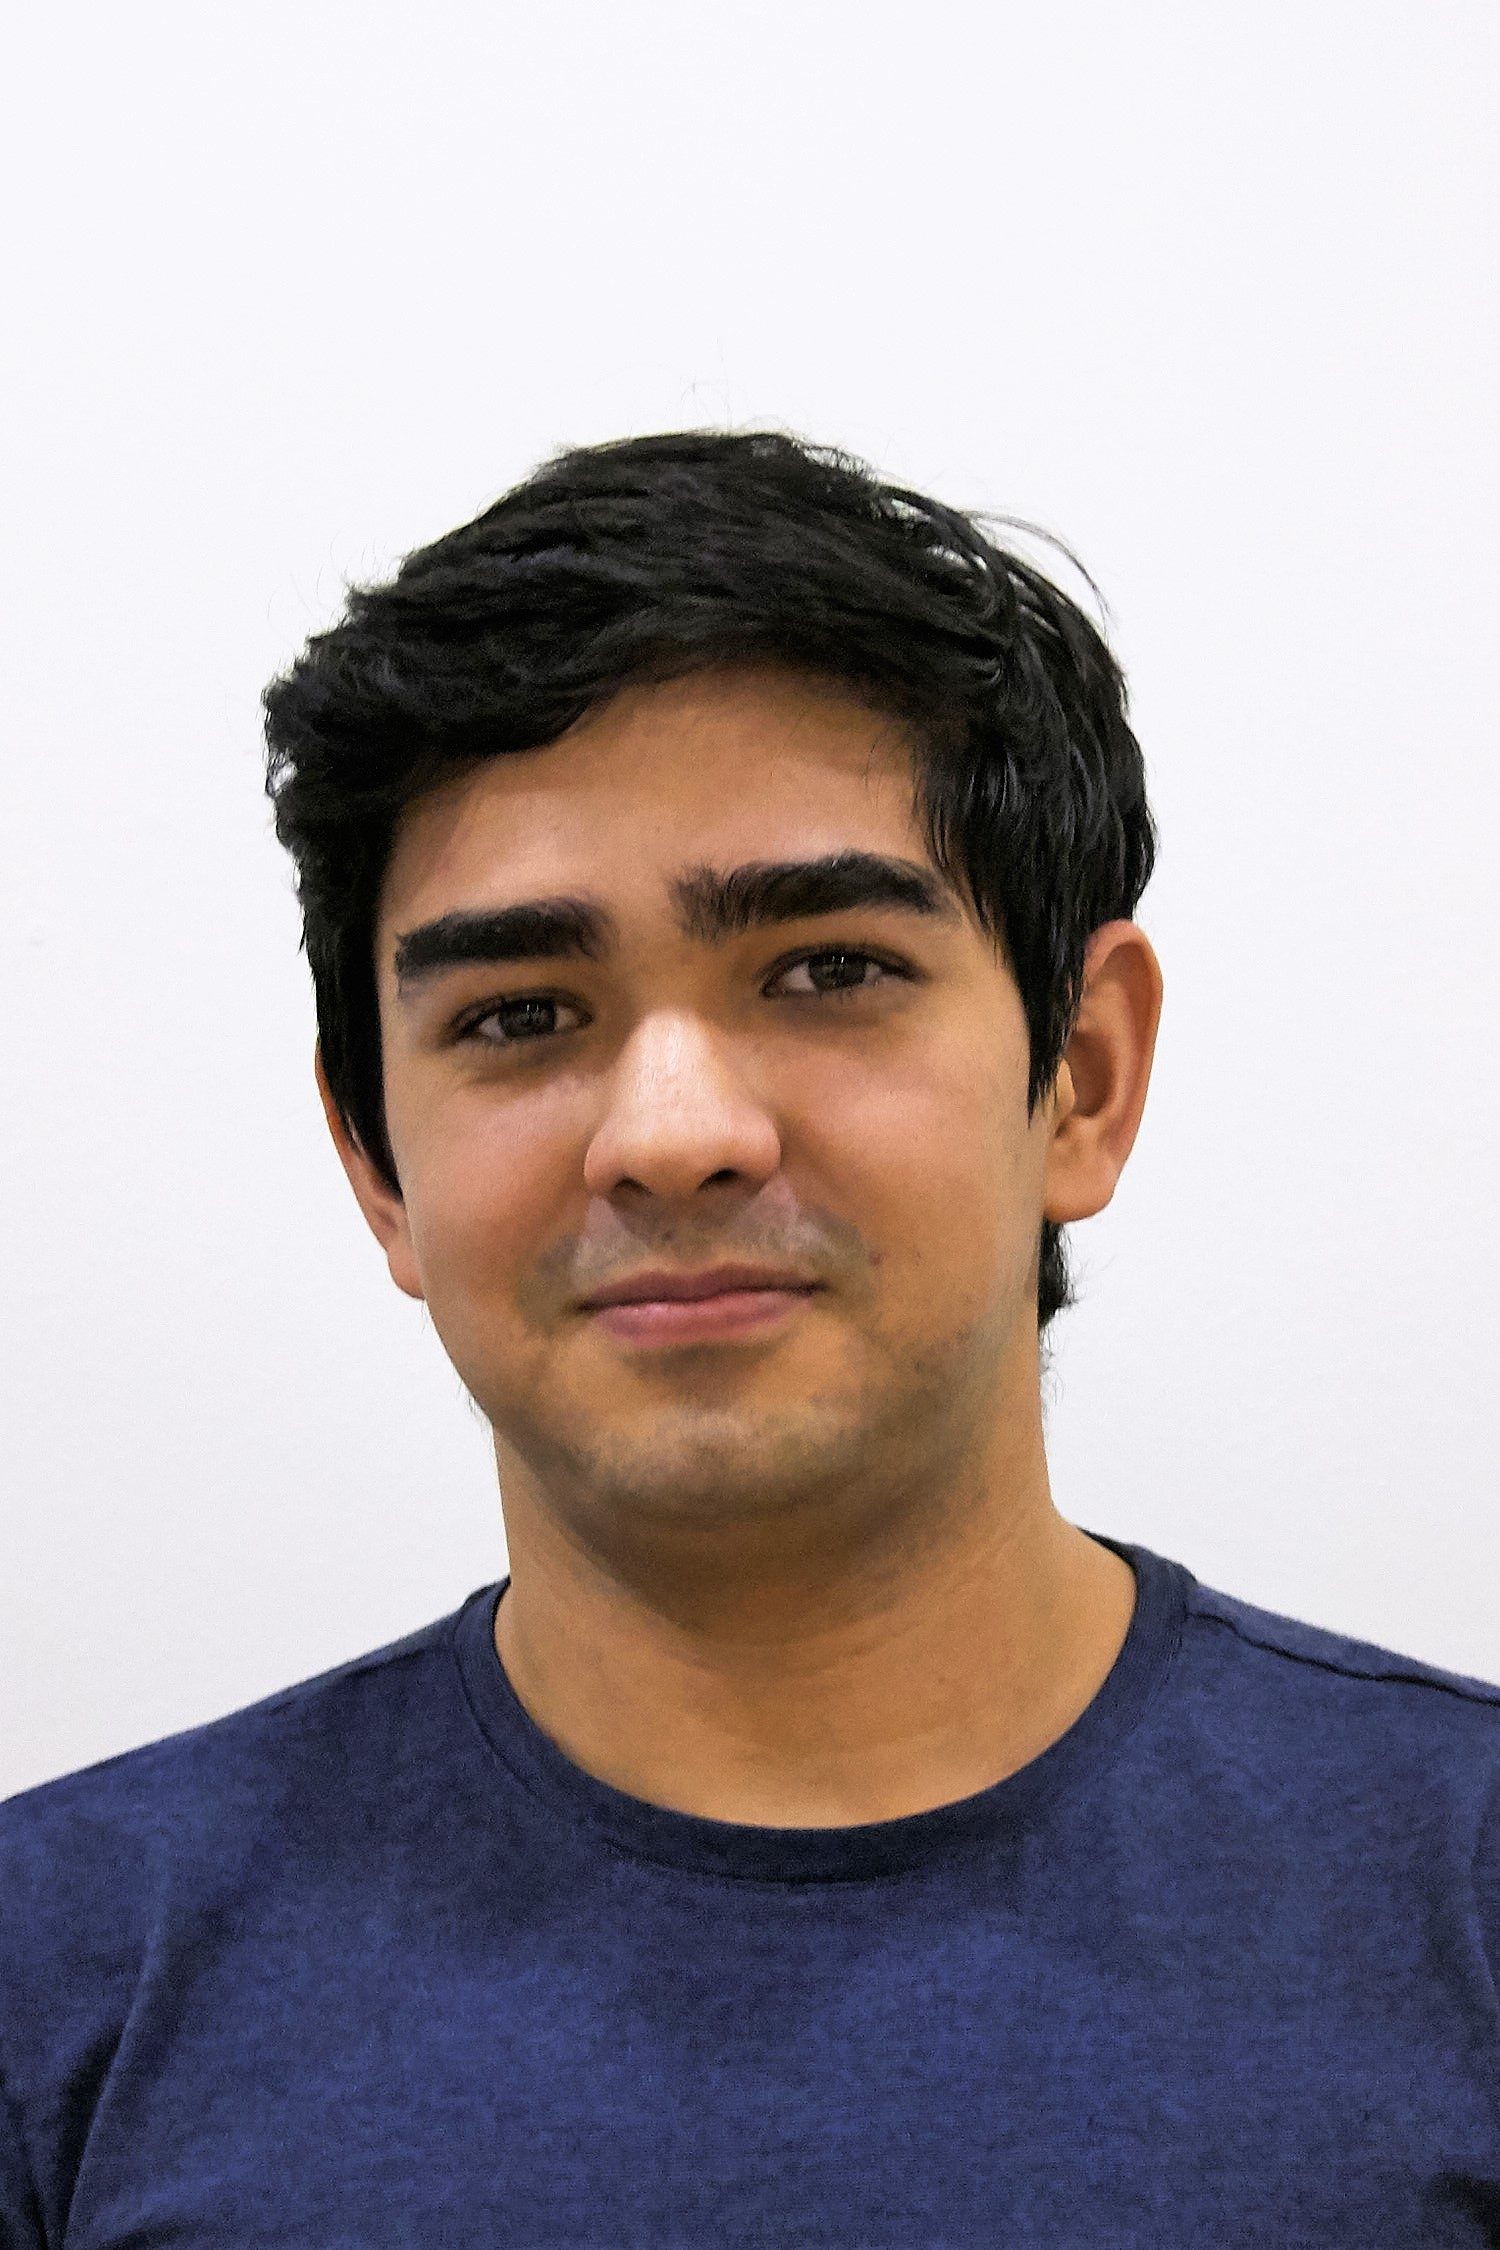
\includegraphics[width=0.2\textwidth]{0-cover/img/TEAMPICS/Diego_final.jpg} & \textbf{Diego Octavio Talavera Maya - Management}

\smallskip
\textit{Current Education}: MSc in Space Sciences and Technology (SpaceMaster).

\smallskip
\textit{Previous Education}: BSc in Aerospace Engineering at the Autonomous University of Baja California (UABC).

\smallskip
\textit{Responsibilities}: Project Management, Mechanical.
\bigskip
\\

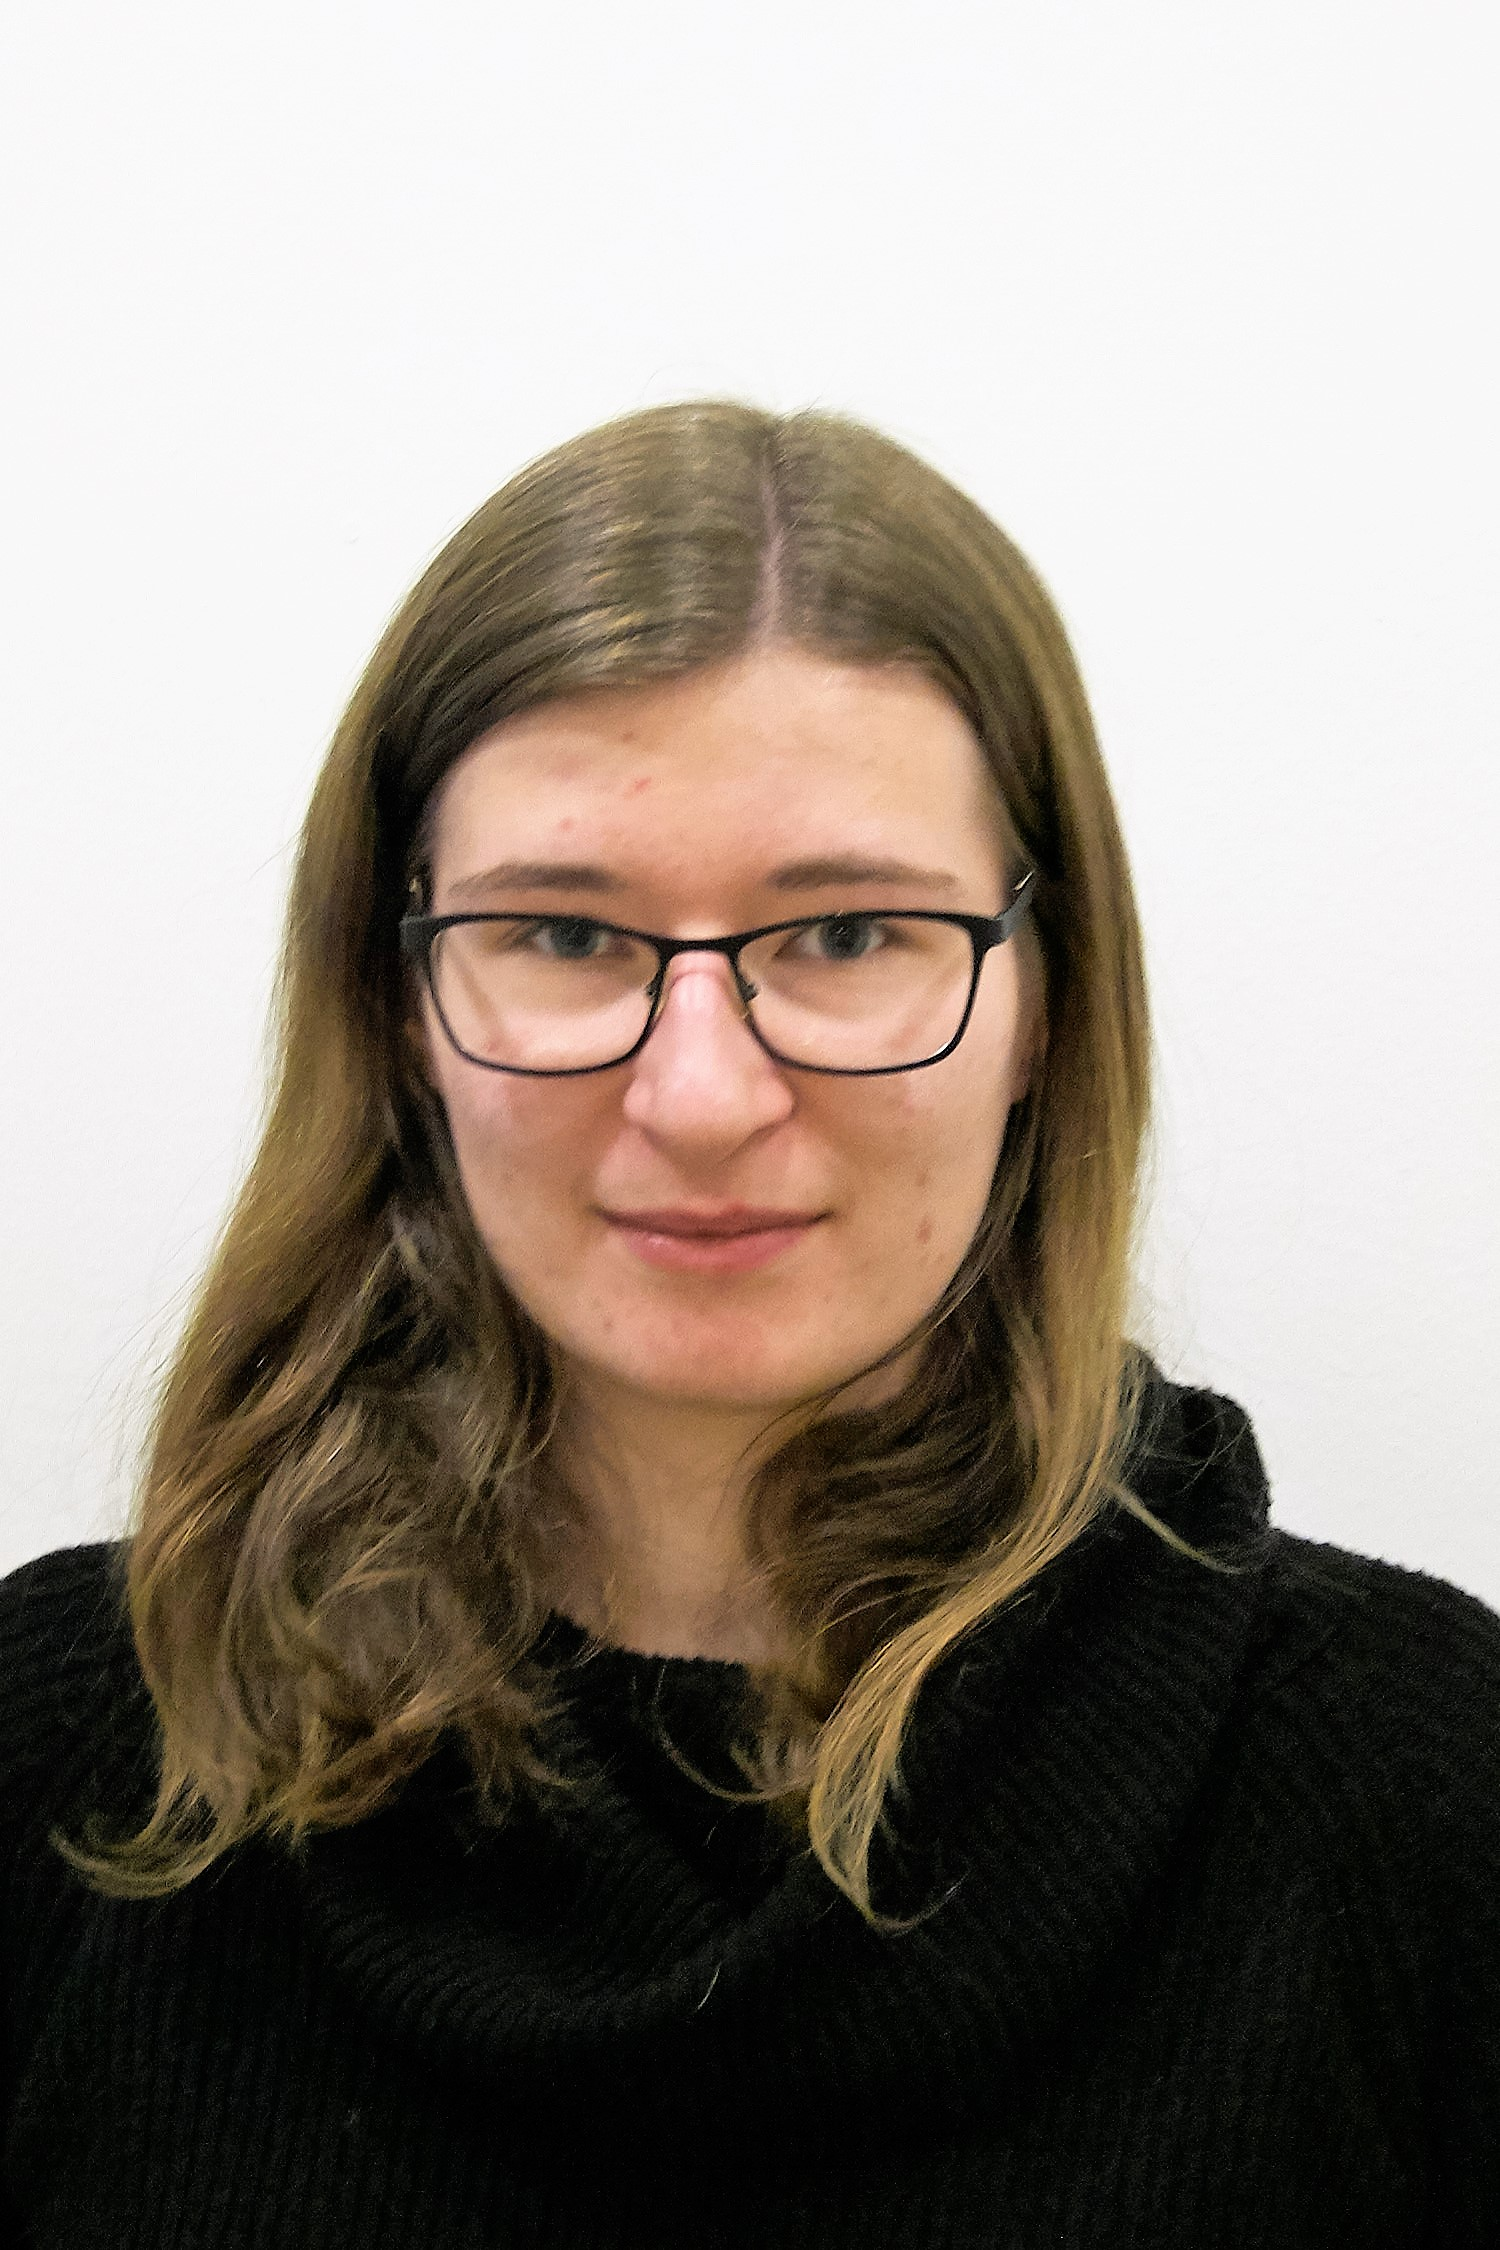
\includegraphics[width=0.2\textwidth]{0-cover/img/TEAMPICS/Anja_final.jpg}  & \textbf{Anja M\"oslinger - Control system}

\smallskip
\textit{Current Education}: MSc in Space Sciences and Technology (SpaceMaster).

\smallskip
\textit{Previous Education}: BSc in Mechatronics at the Johannes Kepler University (JKU)

\smallskip
\textit{Responsibilities}: Control system, Stabilisation system, Camera system
\bigskip
\\

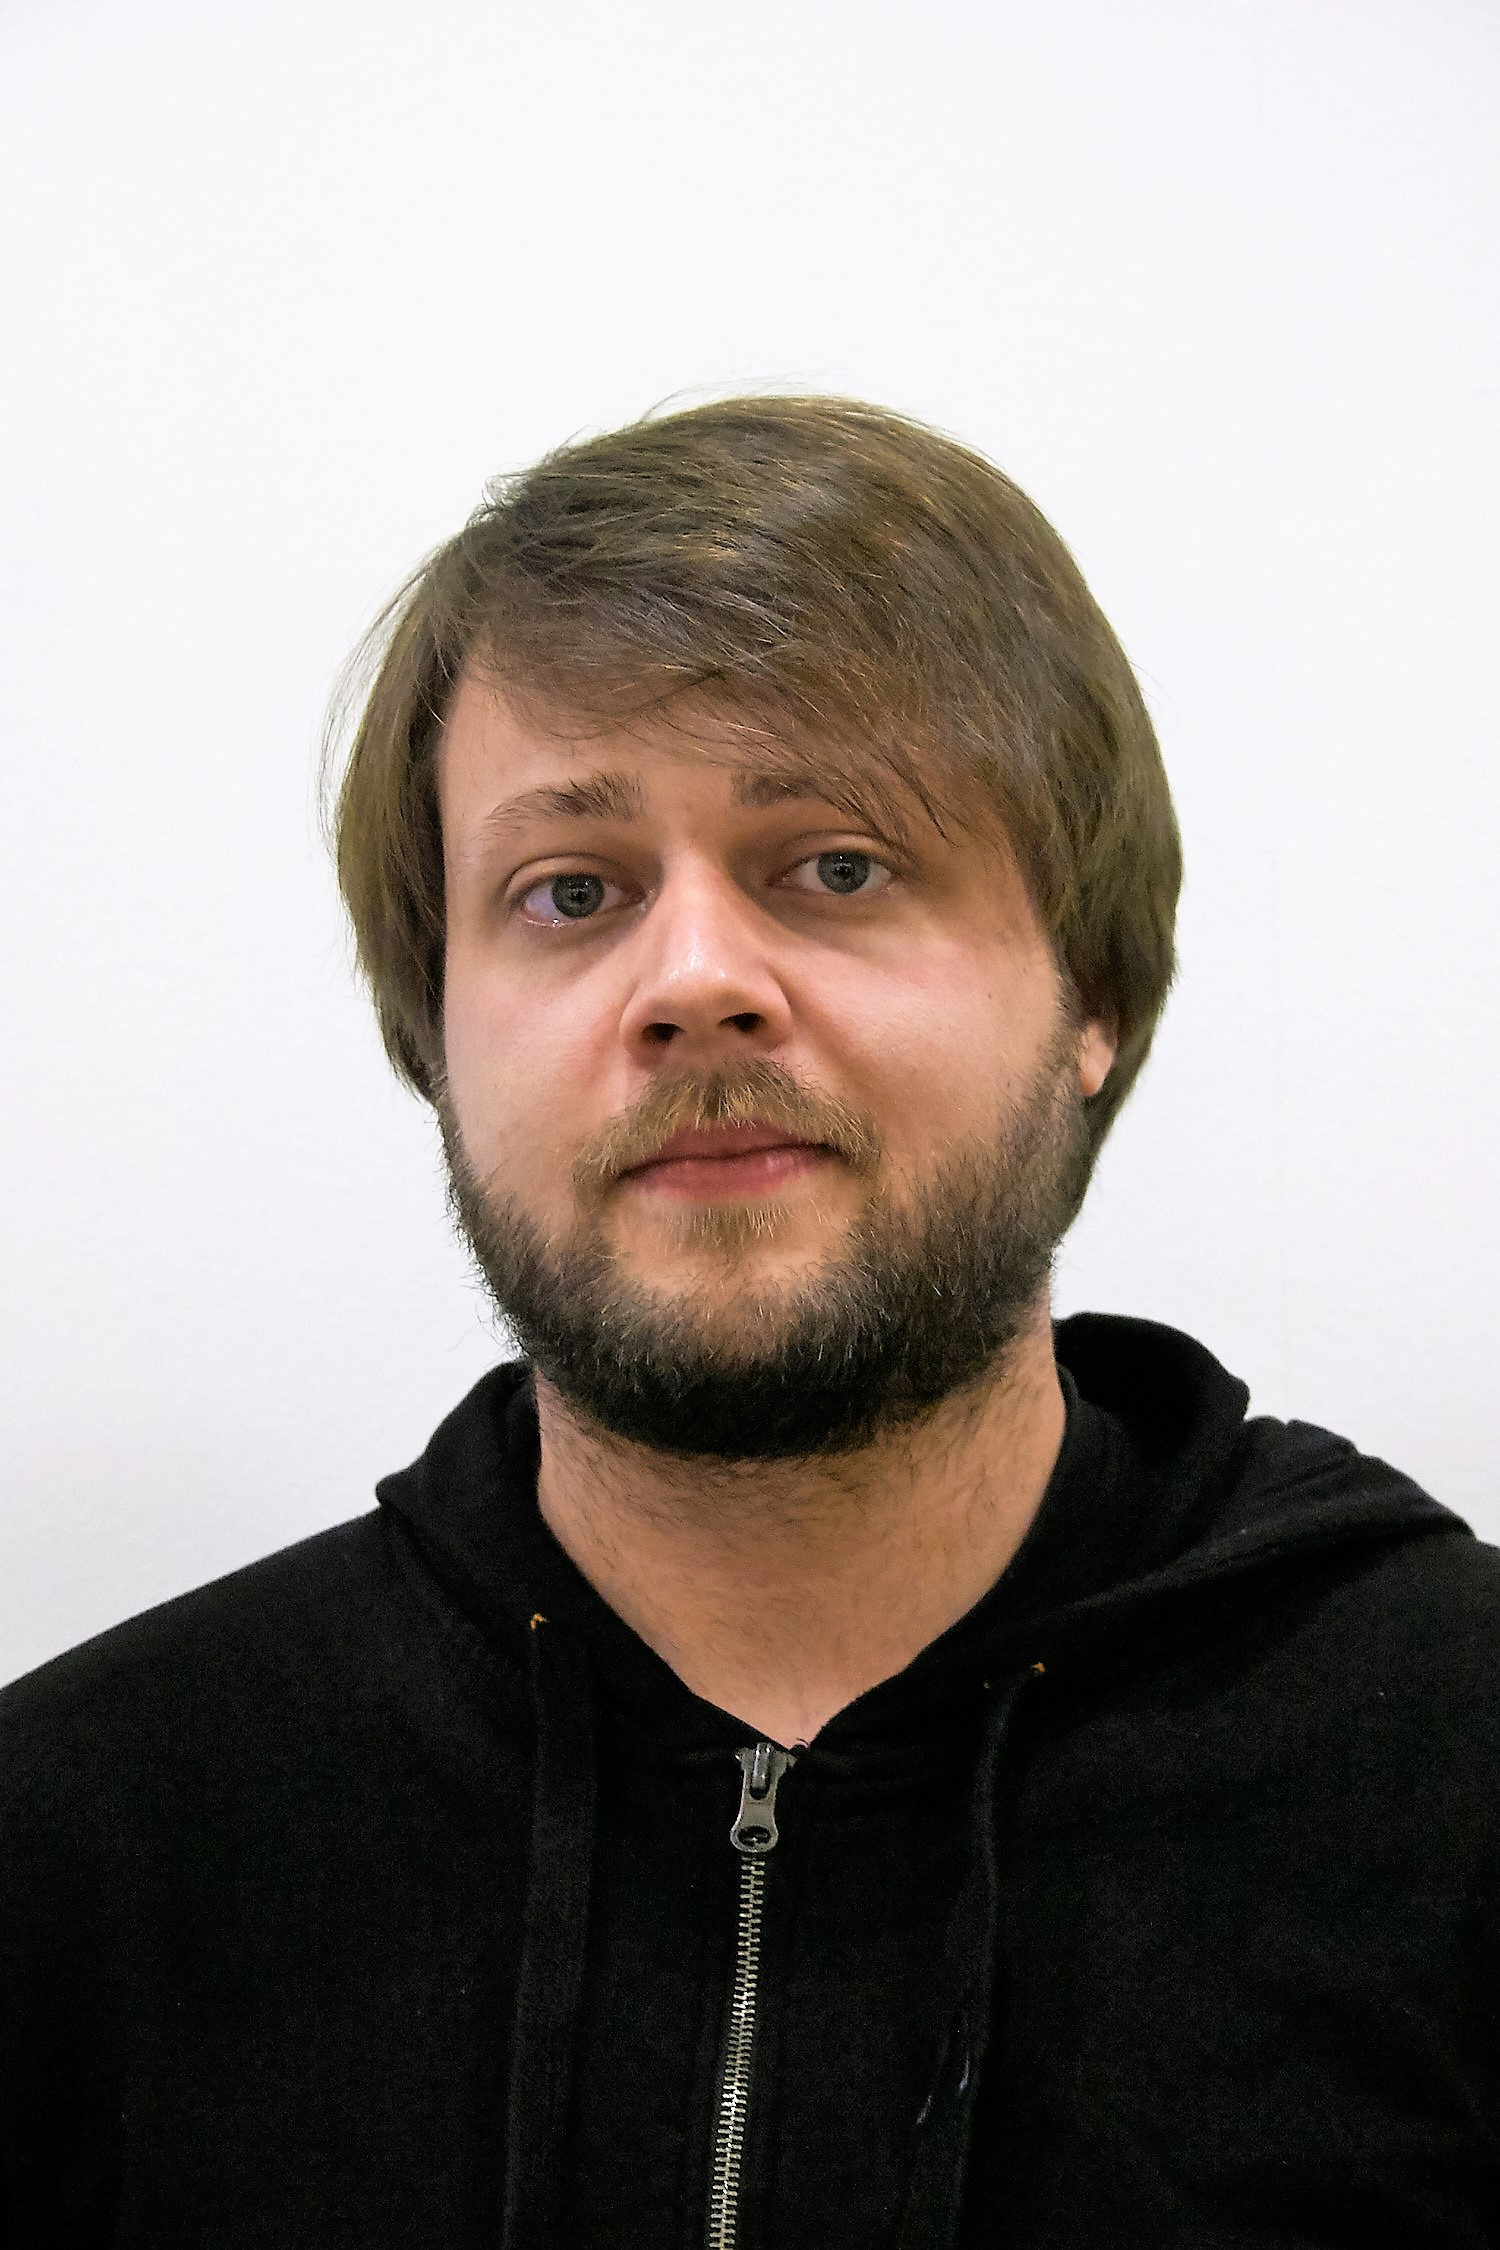
\includegraphics[width=0.2\textwidth]{0-cover/img/TEAMPICS/Elrick_final.jpg}  & \textbf{Eligius Franciscus Maria Weterings - Electrical}

\smallskip
\textit{Current Education}: MSc in Space Sciences and Technology (SpaceMaster).

\smallskip
\textit{Previous Education}: BSc in electrical engineering at the University of Rotterdam (HR) with a specialization in computer sciences and mathematics at the University Utrecht (UU).

\smallskip
\textit{Responsibilities}: Embedded systems, electrical engineering.
\bigskip
\\

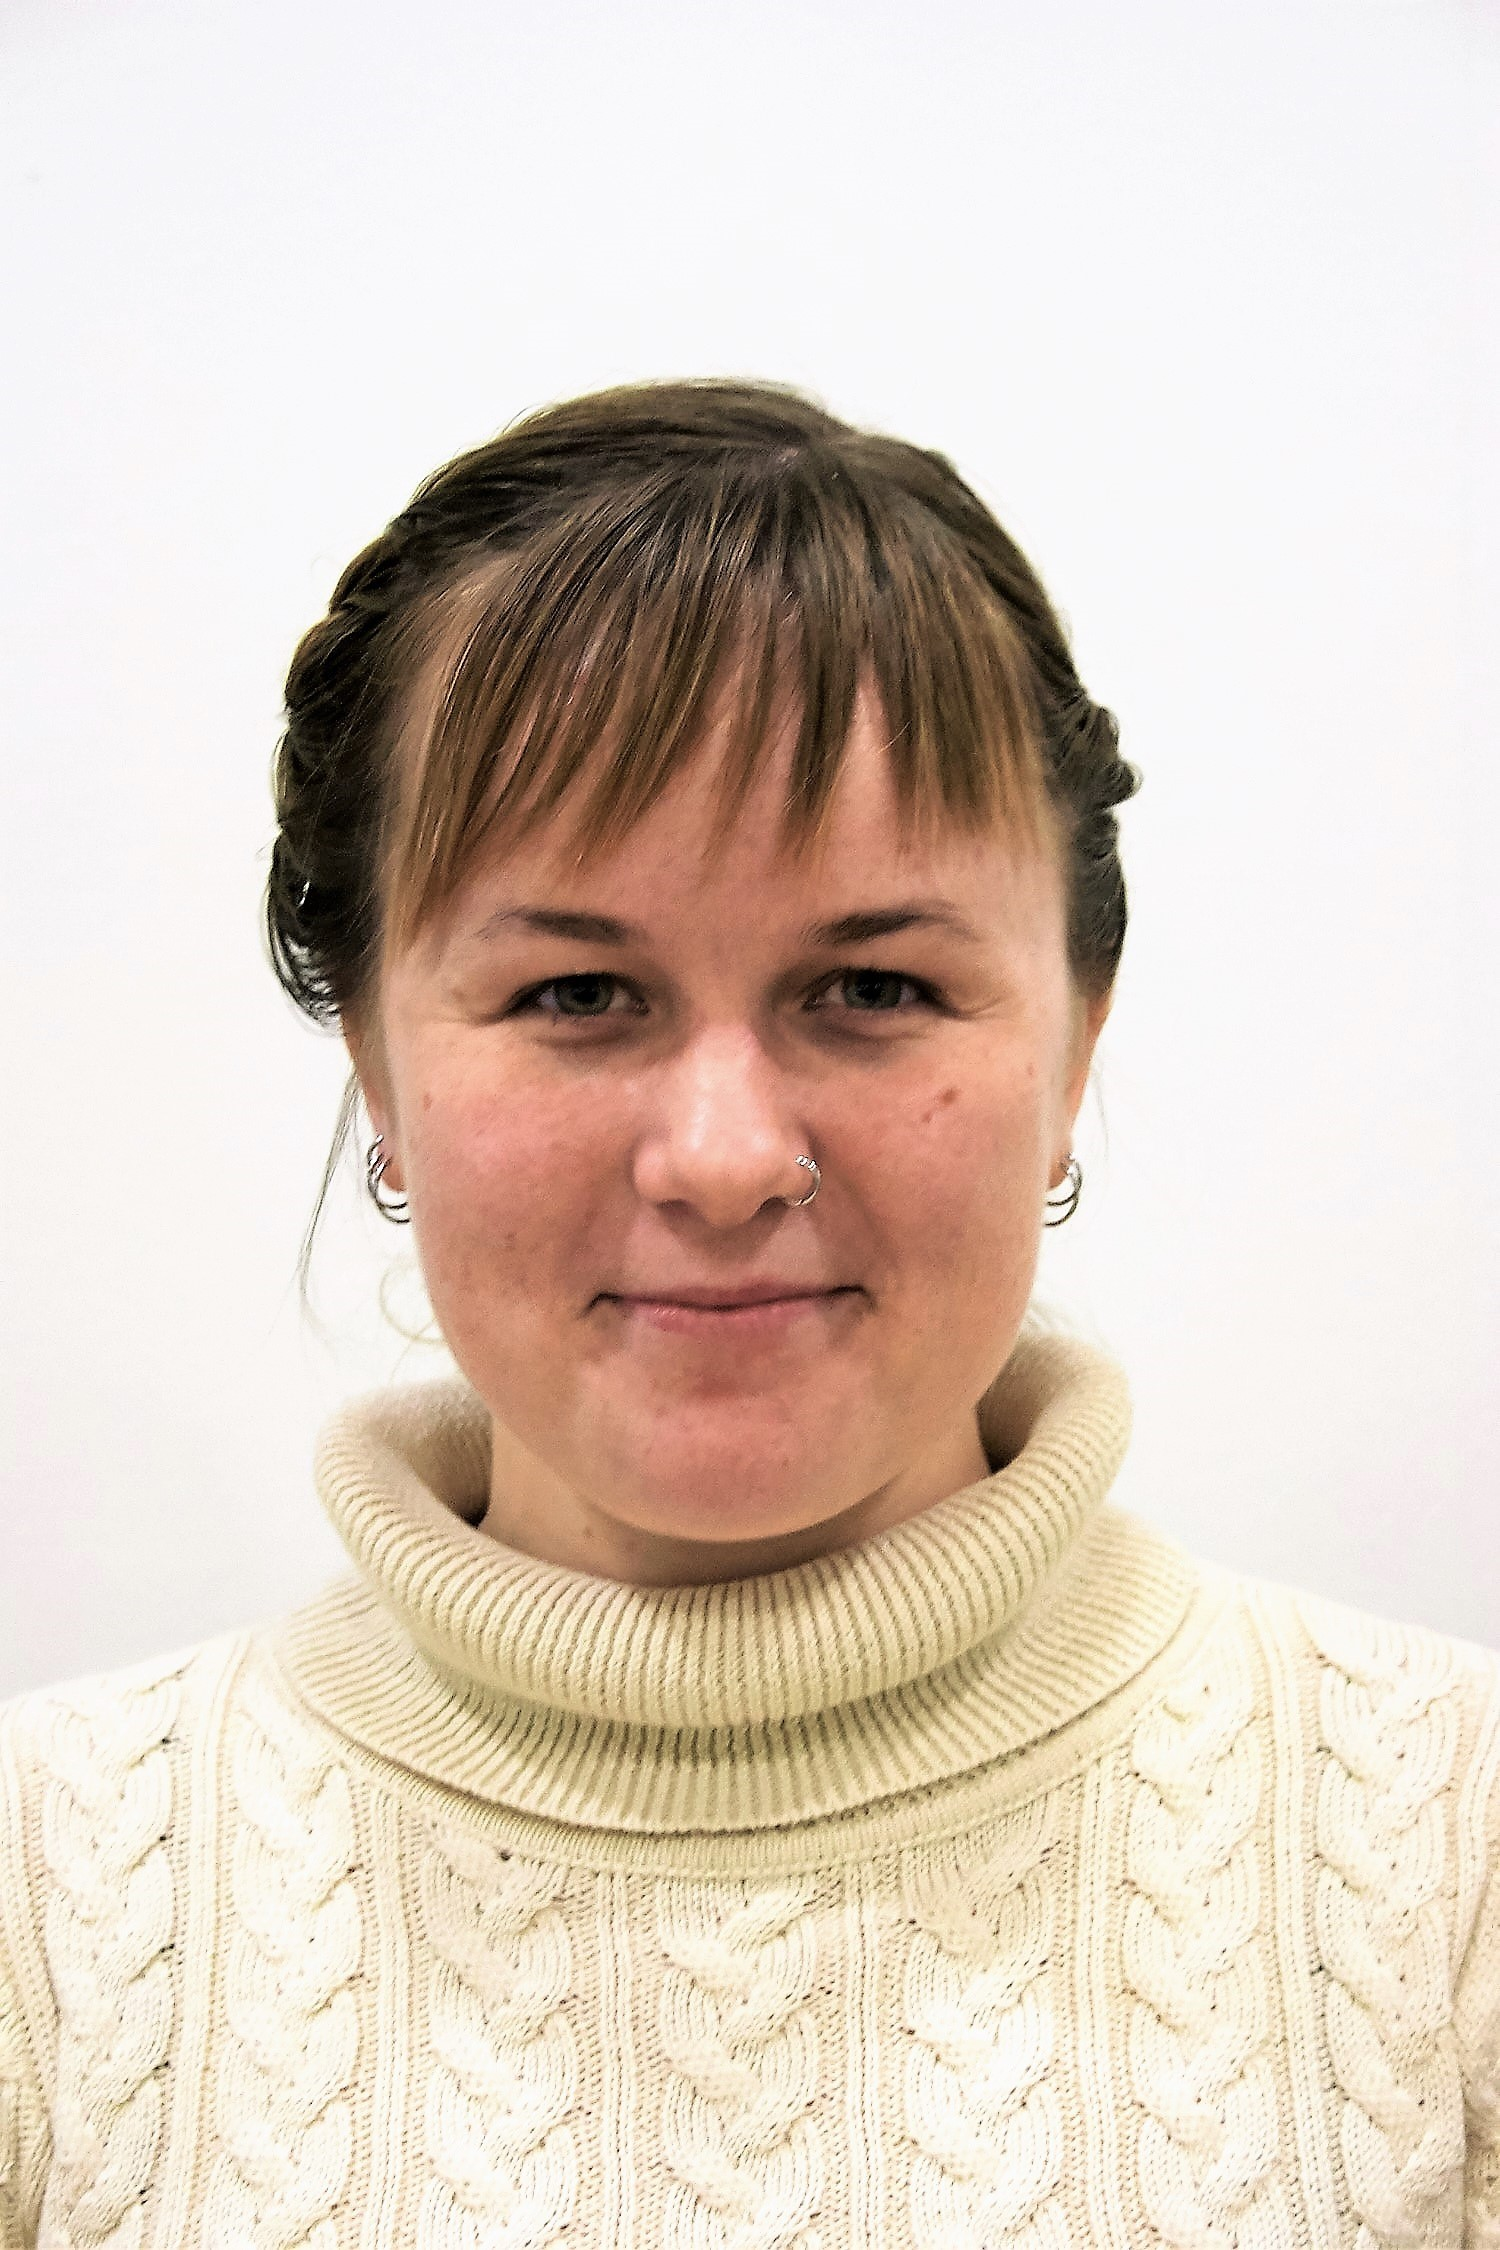
\includegraphics[width=0.2\textwidth]{0-cover/img/TEAMPICS/Kim_Final.jpg}  & \textbf{Kimberly Tuija Steele - Science and Optics}

\smallskip
\textit{Current Education}: MSc in Space Sciences and Technology (SpaceMaster).

\smallskip
\textit{Previous Education}: BSc(Astronomy)(Hons) with a focus on radio astronomy research and instrumentation.

\smallskip
\textit{Responsibilities}: experiment scientific background and overall objectives; defining experimental parameters; data and image analysis; documenting and publishing findings.

\bigskip
\\

  & \st{\textbf{Veronika Haberle - Science}}

\smallskip
\st{\textit{Current Education}: MSc in Space Sciences and Technology (SpaceMaster).}

\smallskip
\st{\textit{Previous Education}:}

\smallskip
\st{\textit{Responsibilities}: Outreach \& data analysis.}
\bigskip
\\

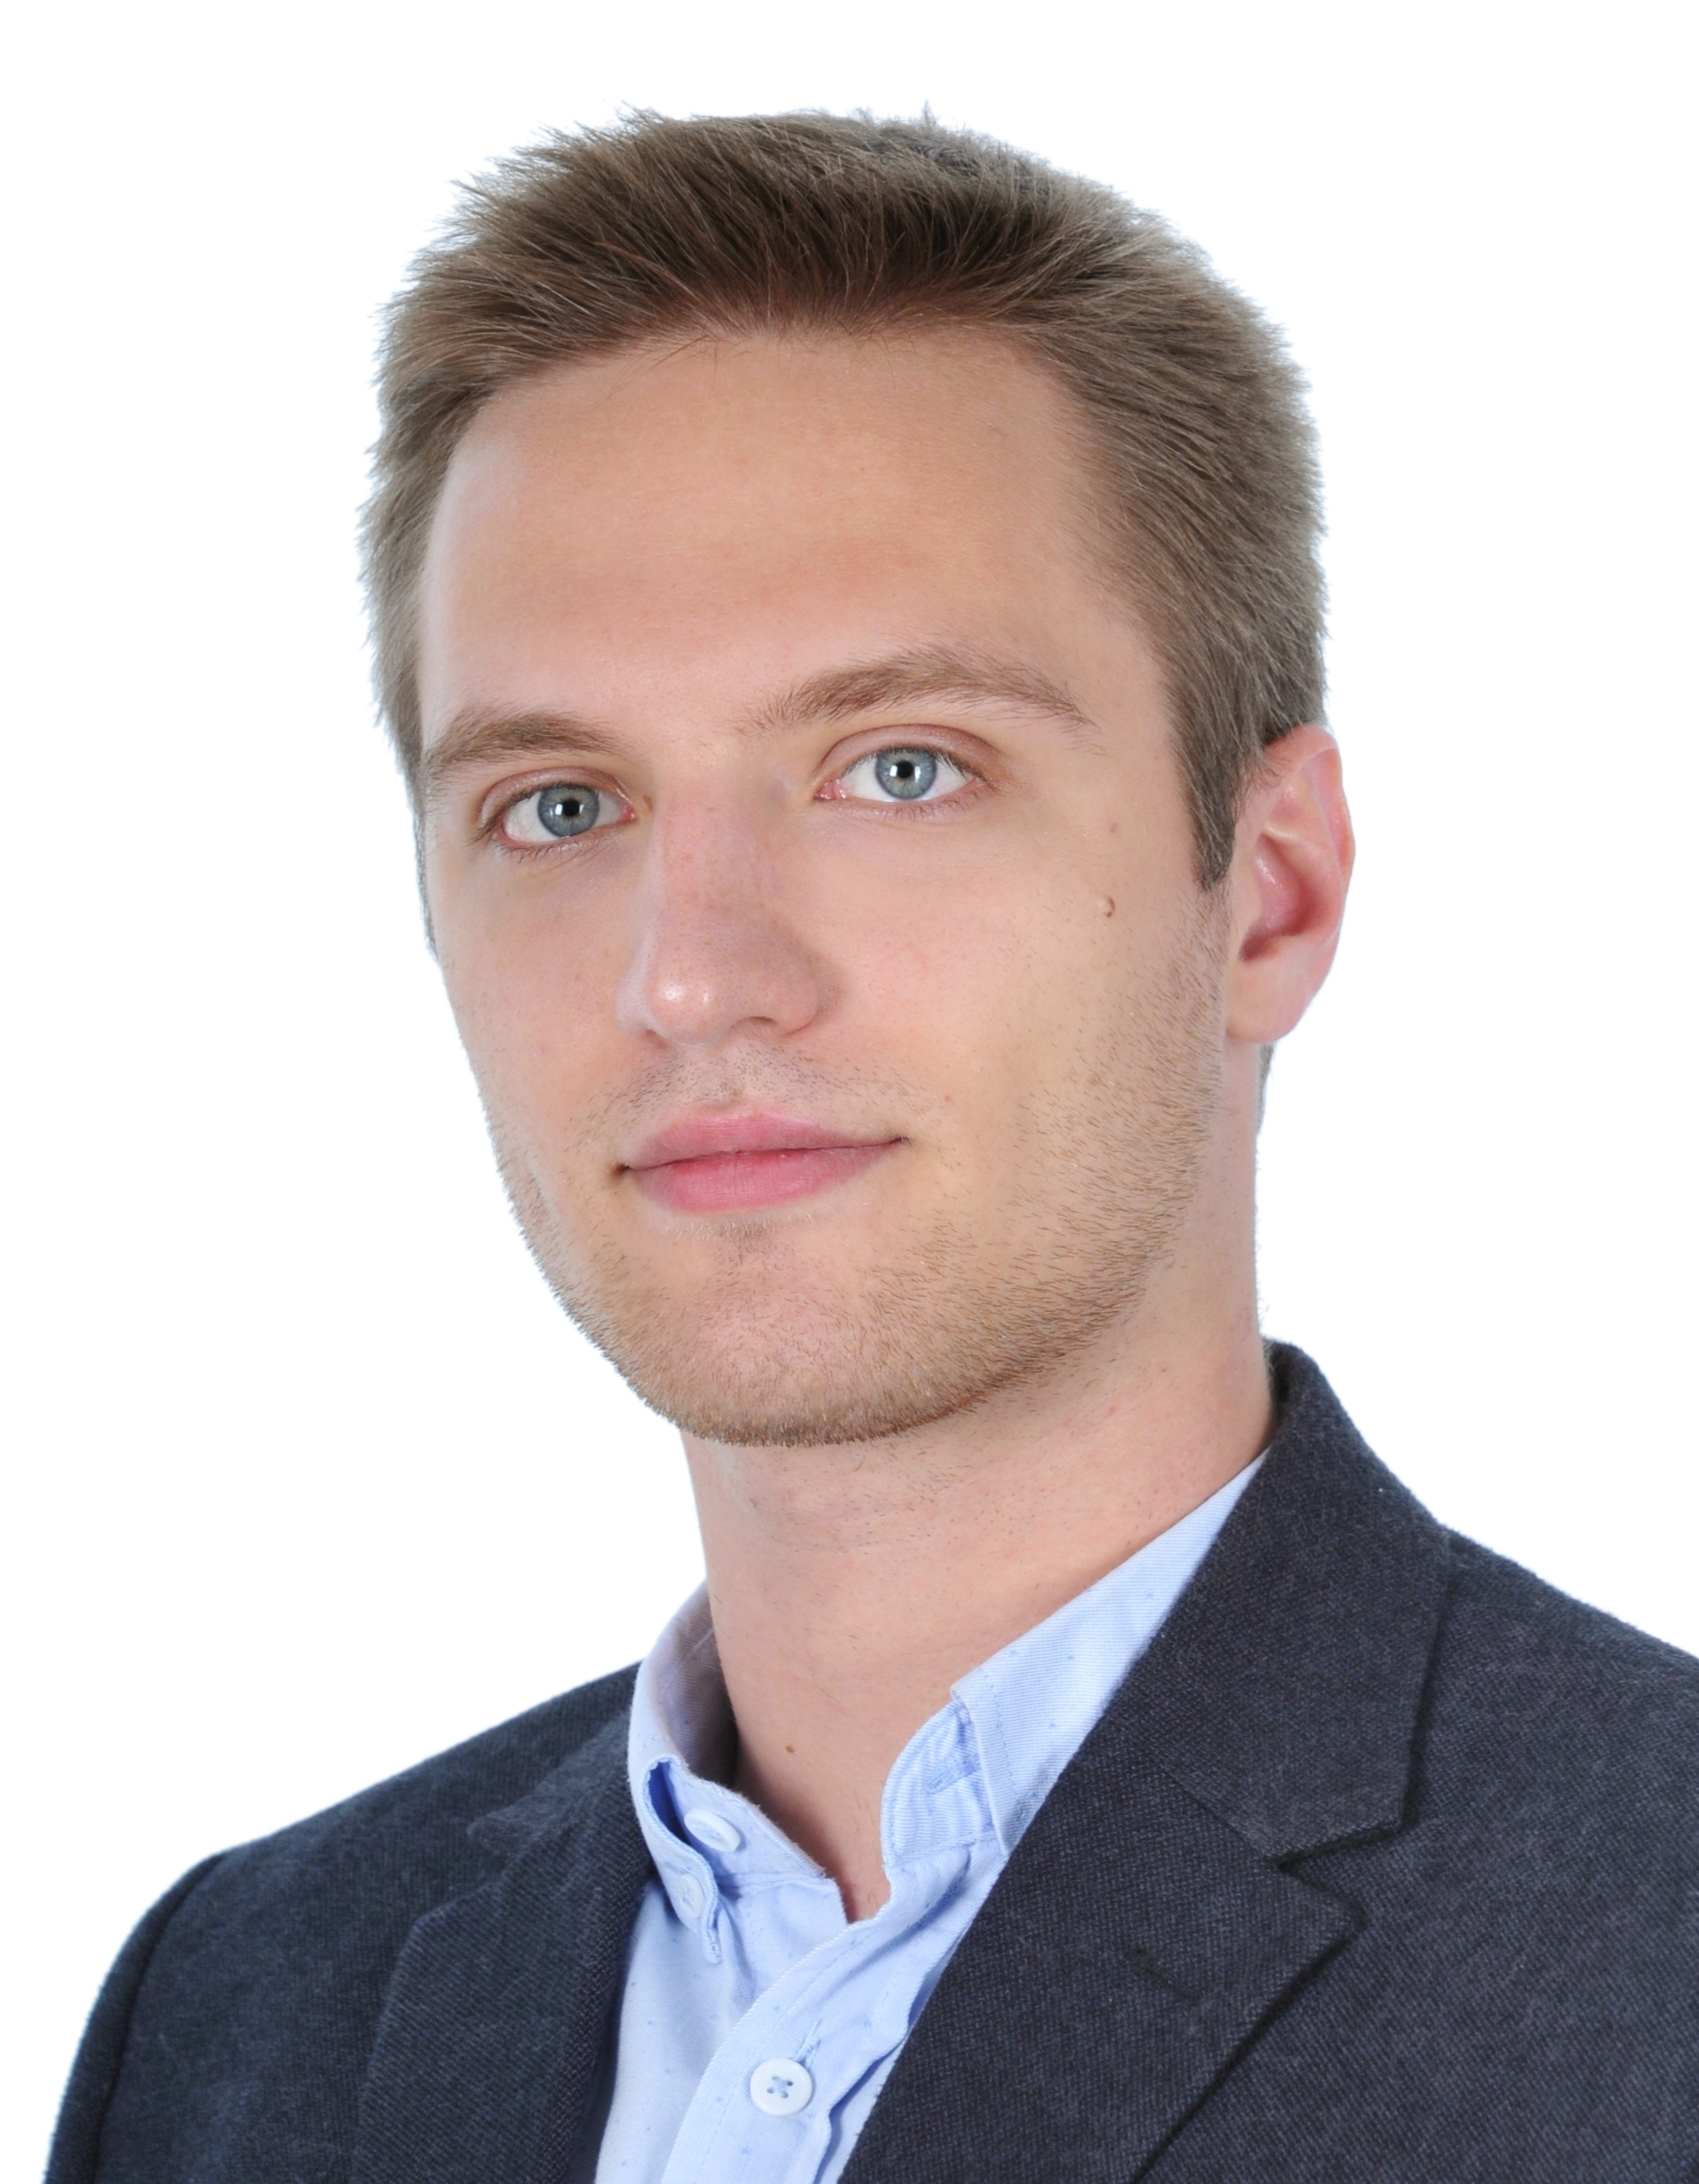
\includegraphics[width=0.2\textwidth]{0-cover/img/TEAMPICS/Adam_final.jpg}  & \textbf{Adam Smialek - Control system}

\smallskip
\textit{Current Education}: MSc in Space Sciences and Technology (SpaceMaster).

\smallskip
\textit{Previous Education}: BSc in Aerospace Engineering at Warsaw University of Technology (WUT) with a specialisation in Automatics and Flight Systems

\smallskip
\textit{Responsibilities}: Onboard control system \& Outreach.
\bigskip
\\

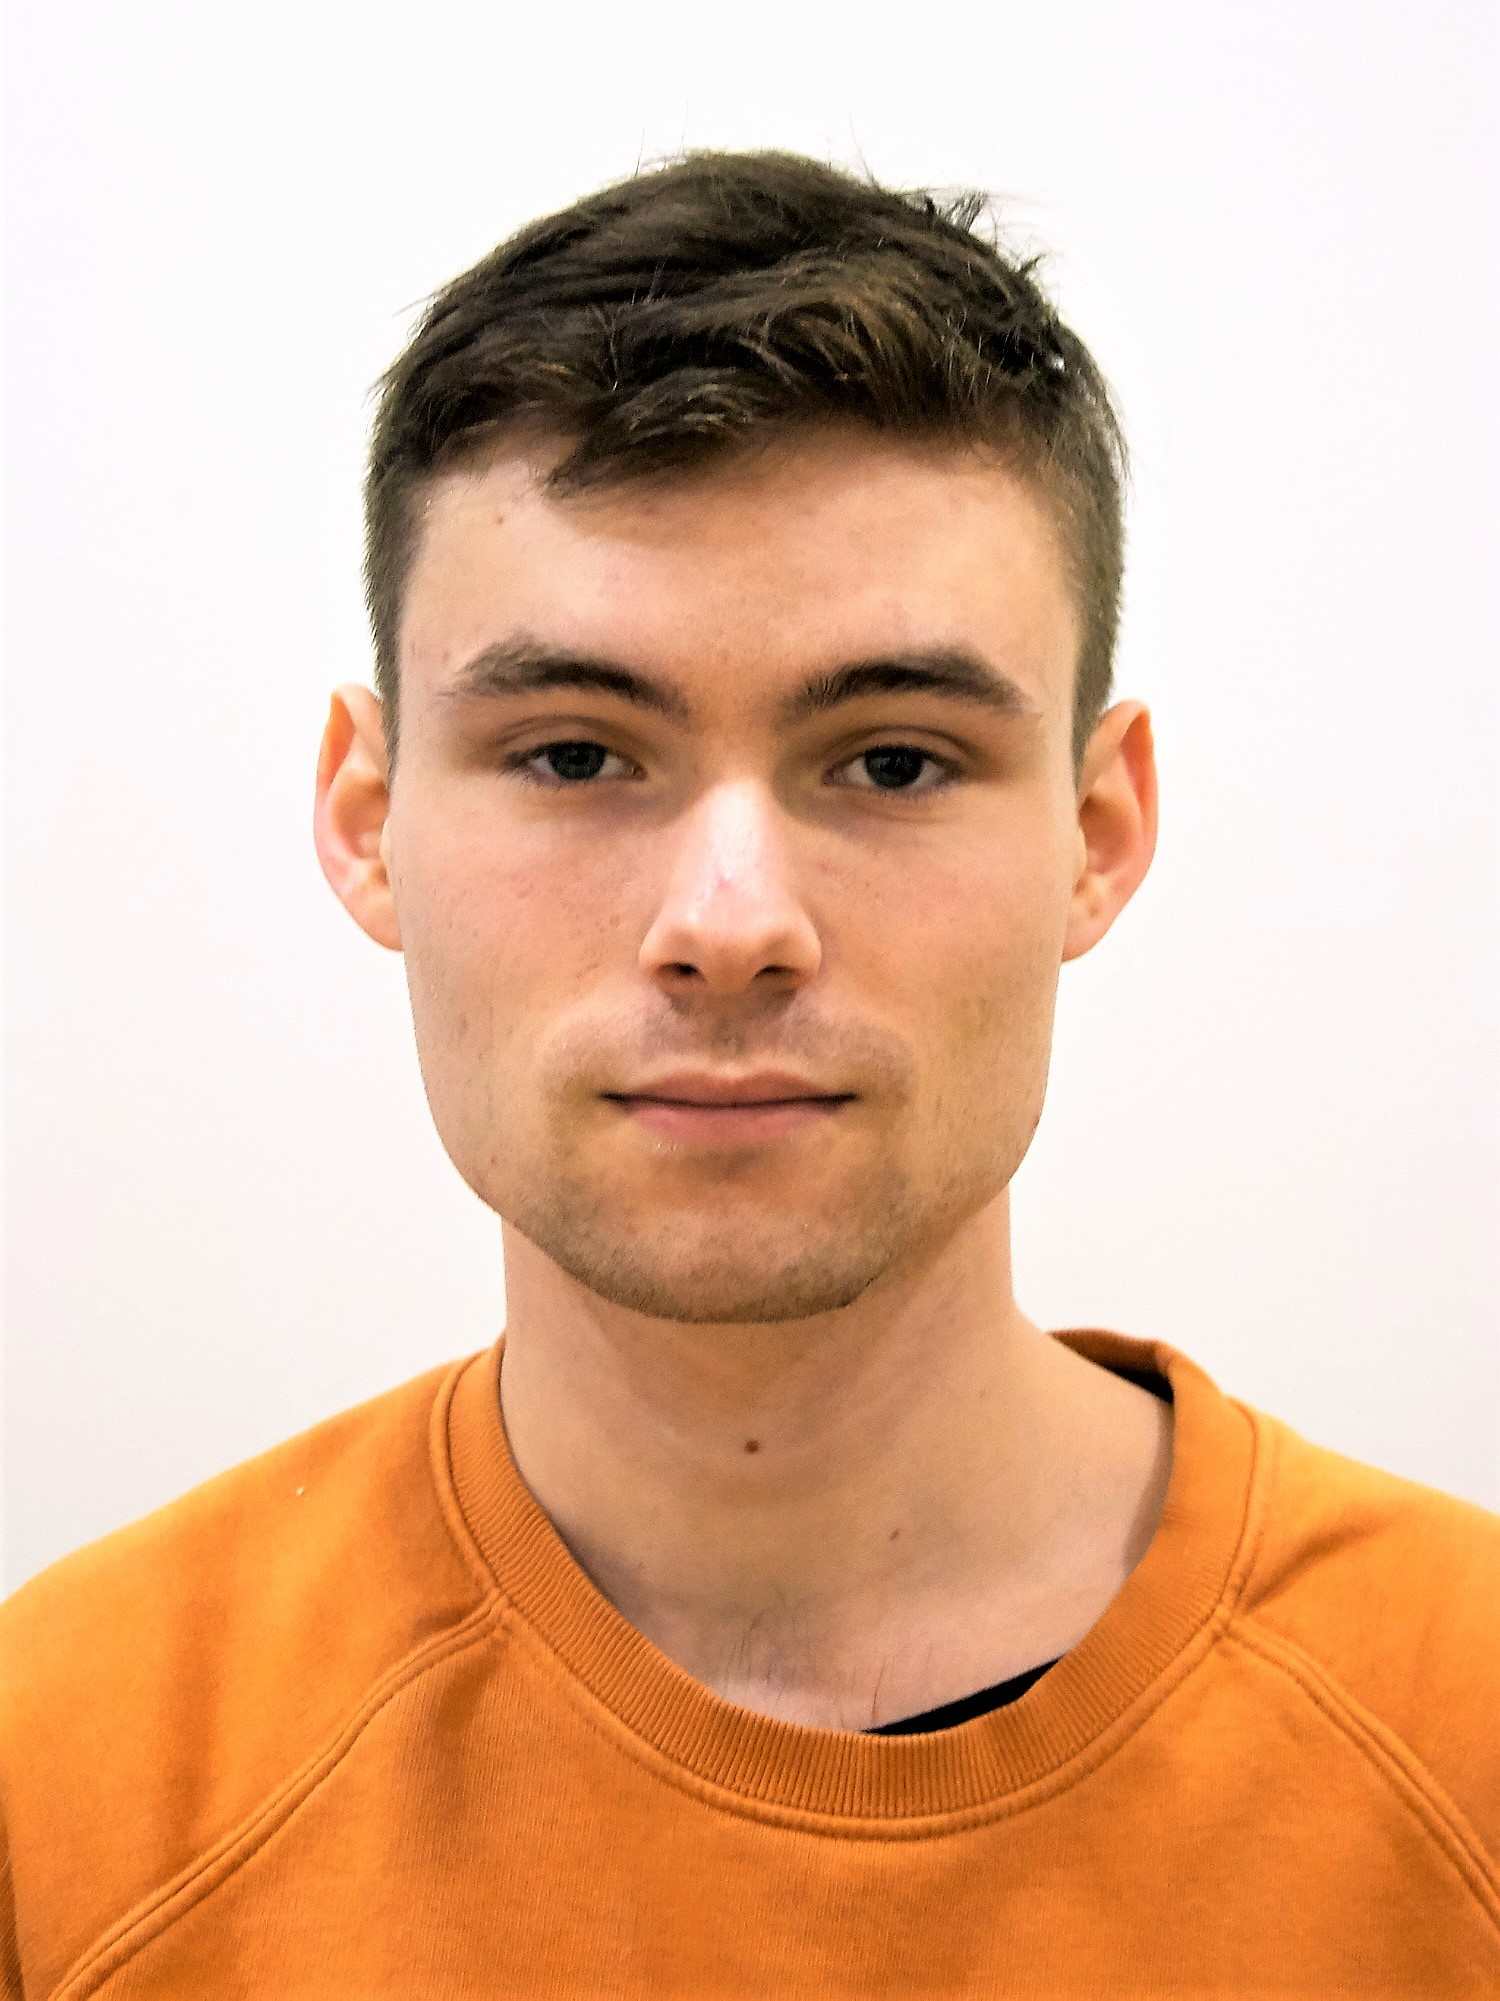
\includegraphics[width=0.2\textwidth]{0-cover/img/TEAMPICS/Jack_Final.jpg}  & \textbf{Jack Hooper - Mechanical}

\smallskip
\textit{Current Education}: MSc in Space Sciences and Technology (SpaceMaster)

\smallskip
\textit{Previous Education}: BEng in Mechanical and Aerospace Engineering at the University of Adelaide (UoA). 

\smallskip
\textit{Responsibilities}: Optothermal analysis, thermal control systems.
\bigskip
\\


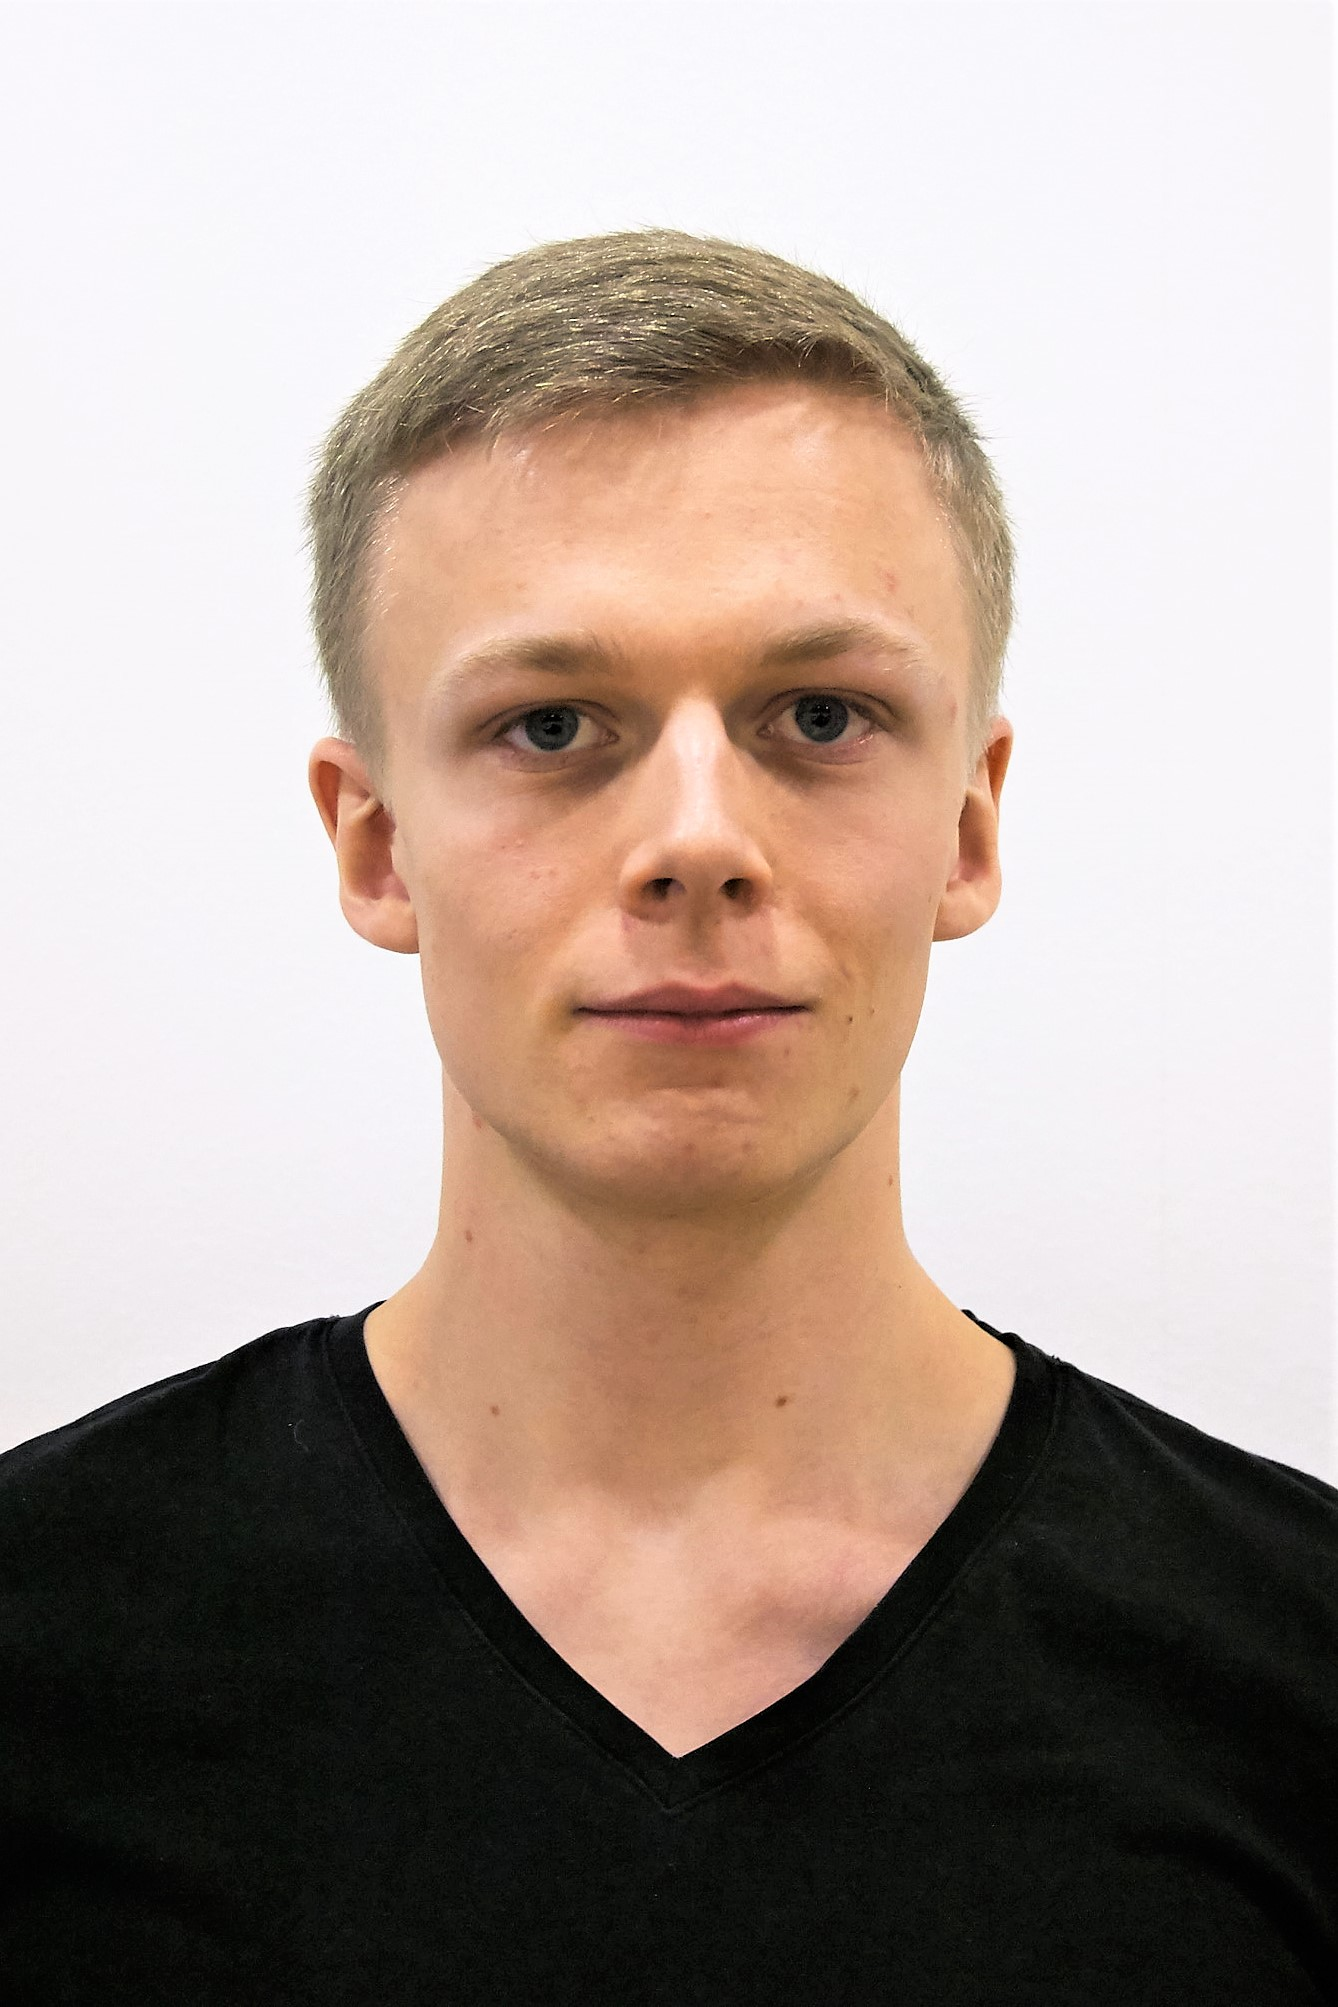
\includegraphics[width=0.2\textwidth]{0-cover/img/TEAMPICS/Harald_final.jpg}  & \textbf{Harald Magnusson - Software}

\smallskip
\textit{Current Education}: Master Programme in Space Engineering, Luleå University of Technology

\smallskip
\textit{Responsibilities}: Software (onboard \& ground station).
\bigskip
\\

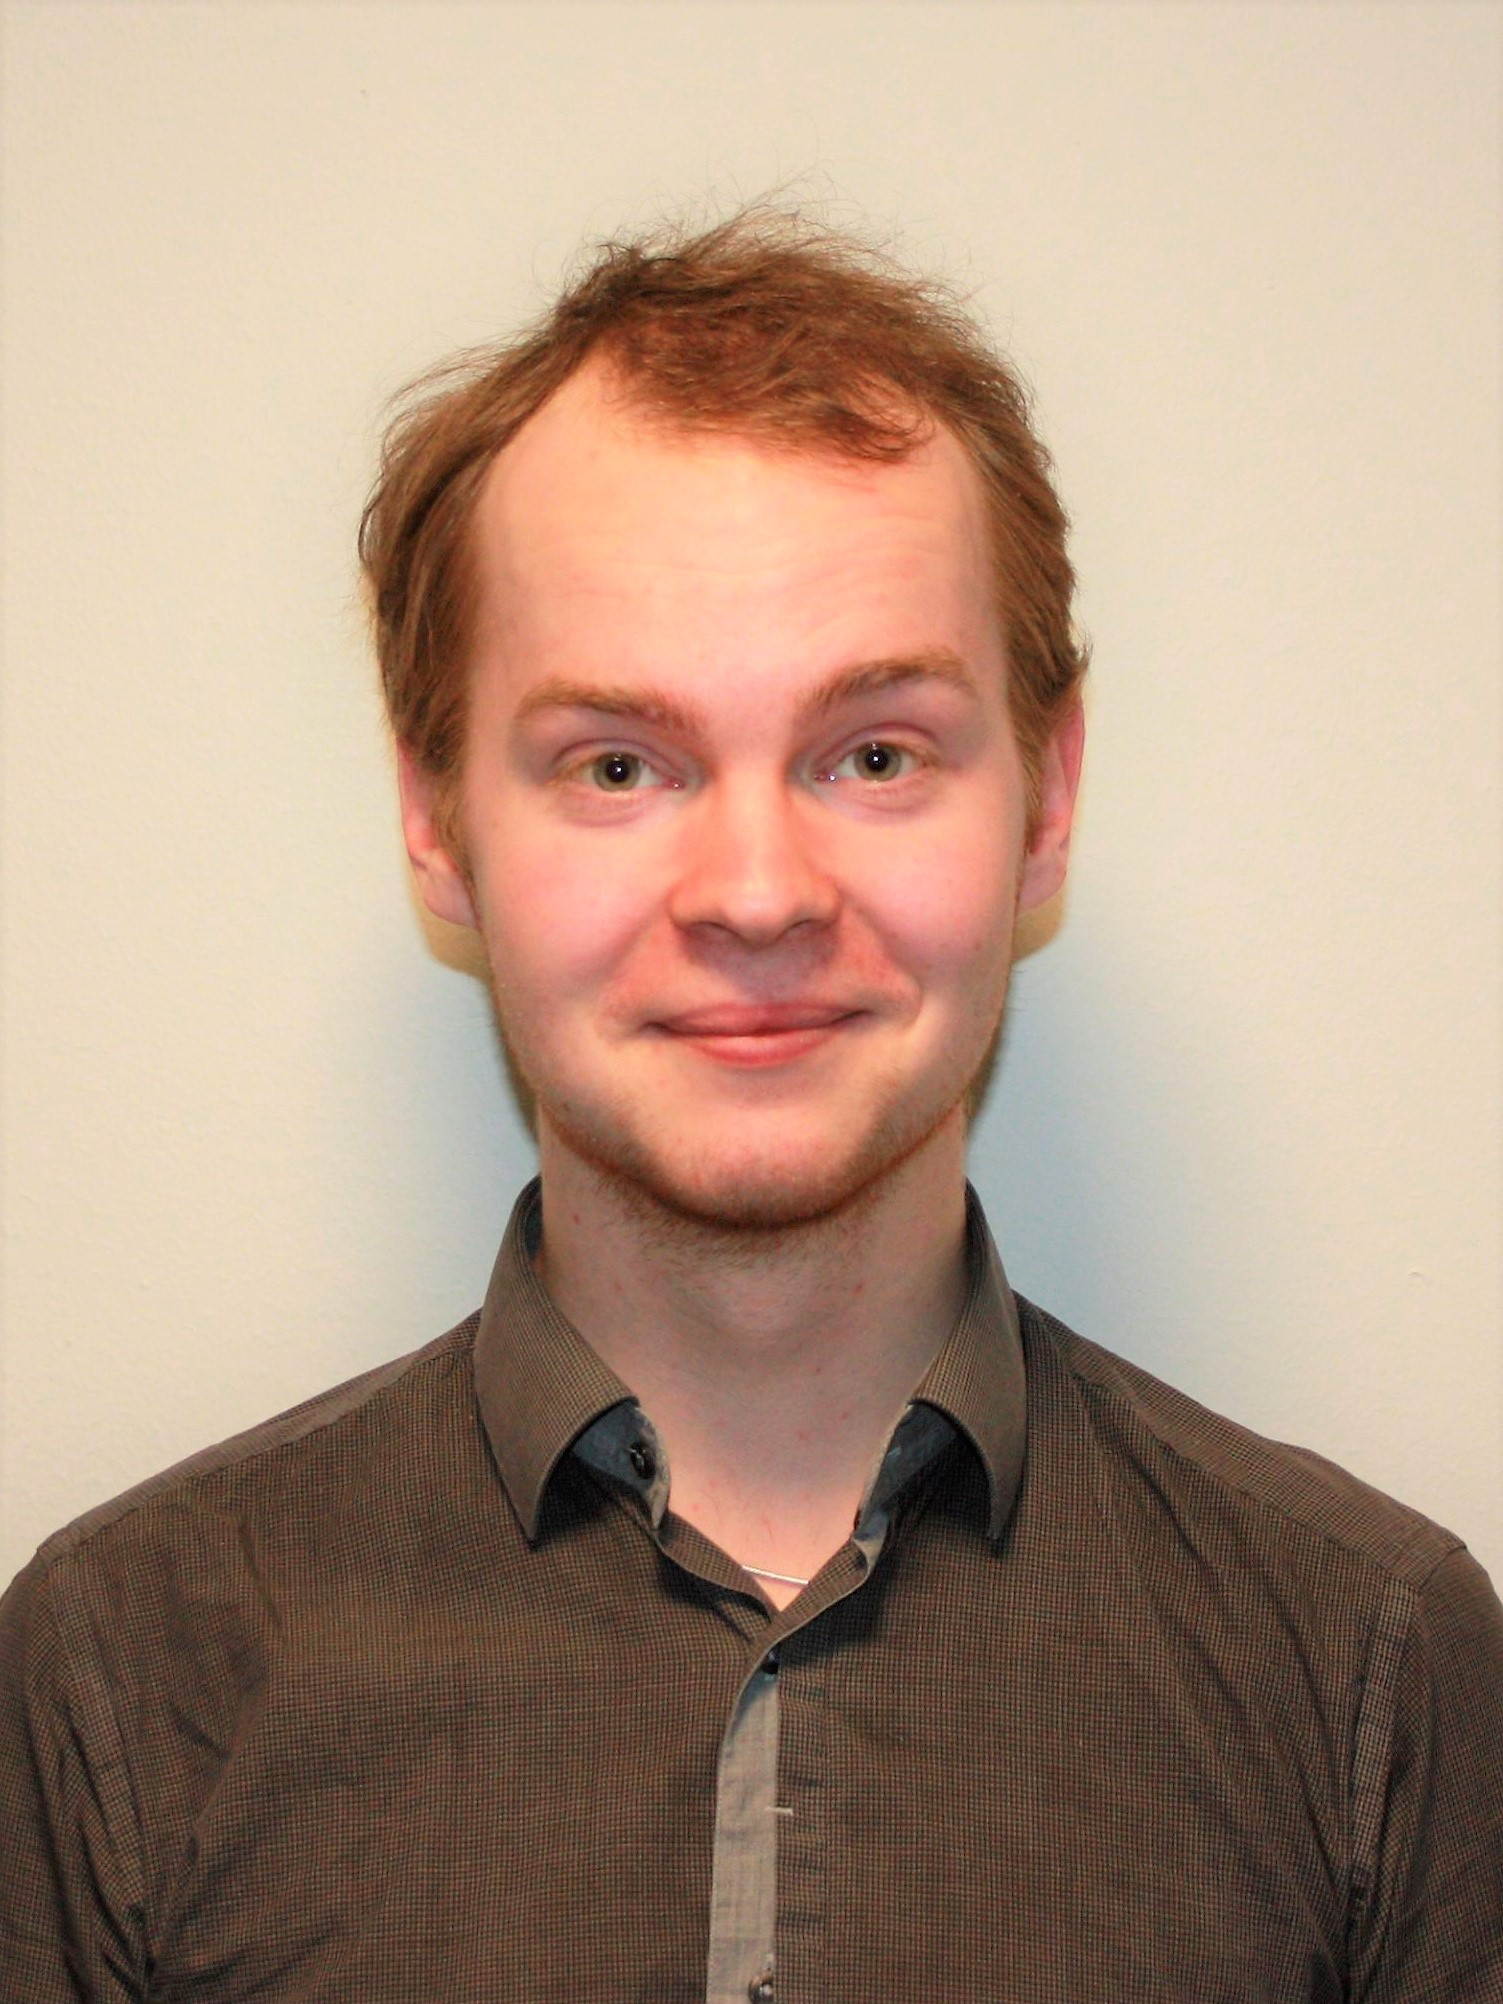
\includegraphics[width=0.2\textwidth]{0-cover/img/TEAMPICS/Niklas_final.jpg}  & \textbf{Niklas Ulfvarson - Software}

\smallskip
\textit{Current Education}: Master Programme in Space Engineering, Luleå University of Technology

\smallskip
\textit{Responsibilities}: Project Management, Software (onboard \& ground station), Star Tracker.
\bigskip
\\

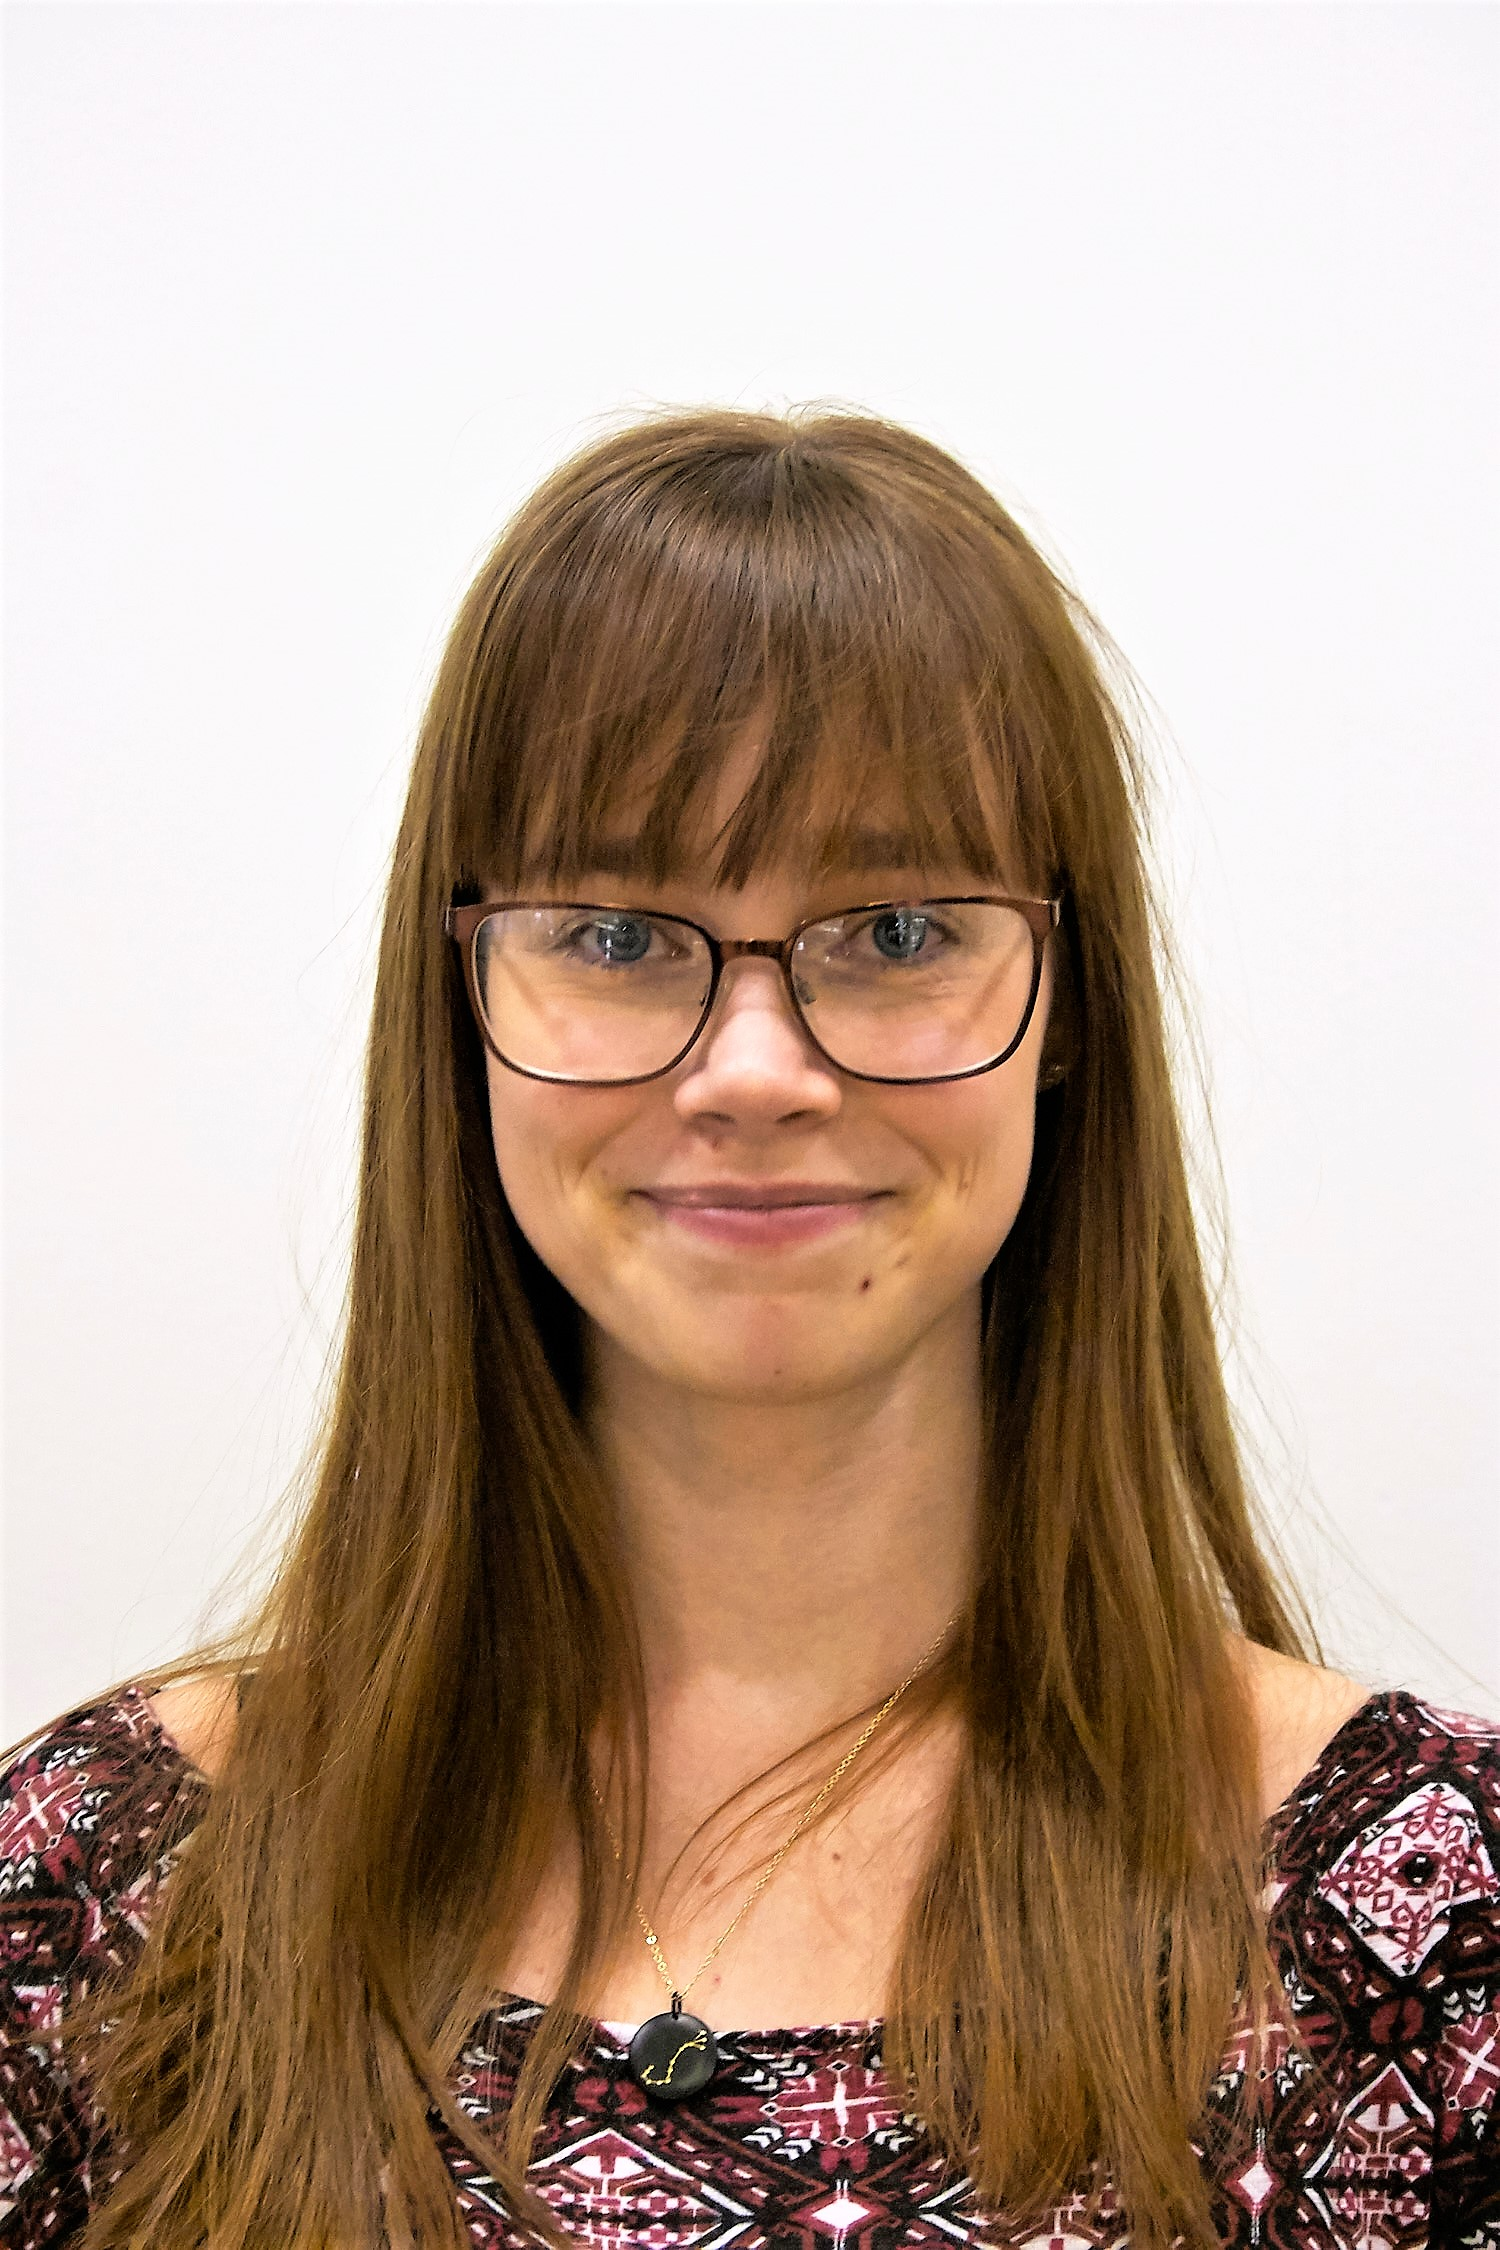
\includegraphics[width=0.2\textwidth]{0-cover/img/TEAMPICS/Sabina_final.jpg}  & \textbf{Sabina Bj\"ork - Electrical}

\smallskip
\textit{Current Education}: Master Programme in Space Engineering, Luleå University of Technology

\smallskip
\textit{Responsibilities}: Energy technology, electrical engineering.
\bigskip
\\

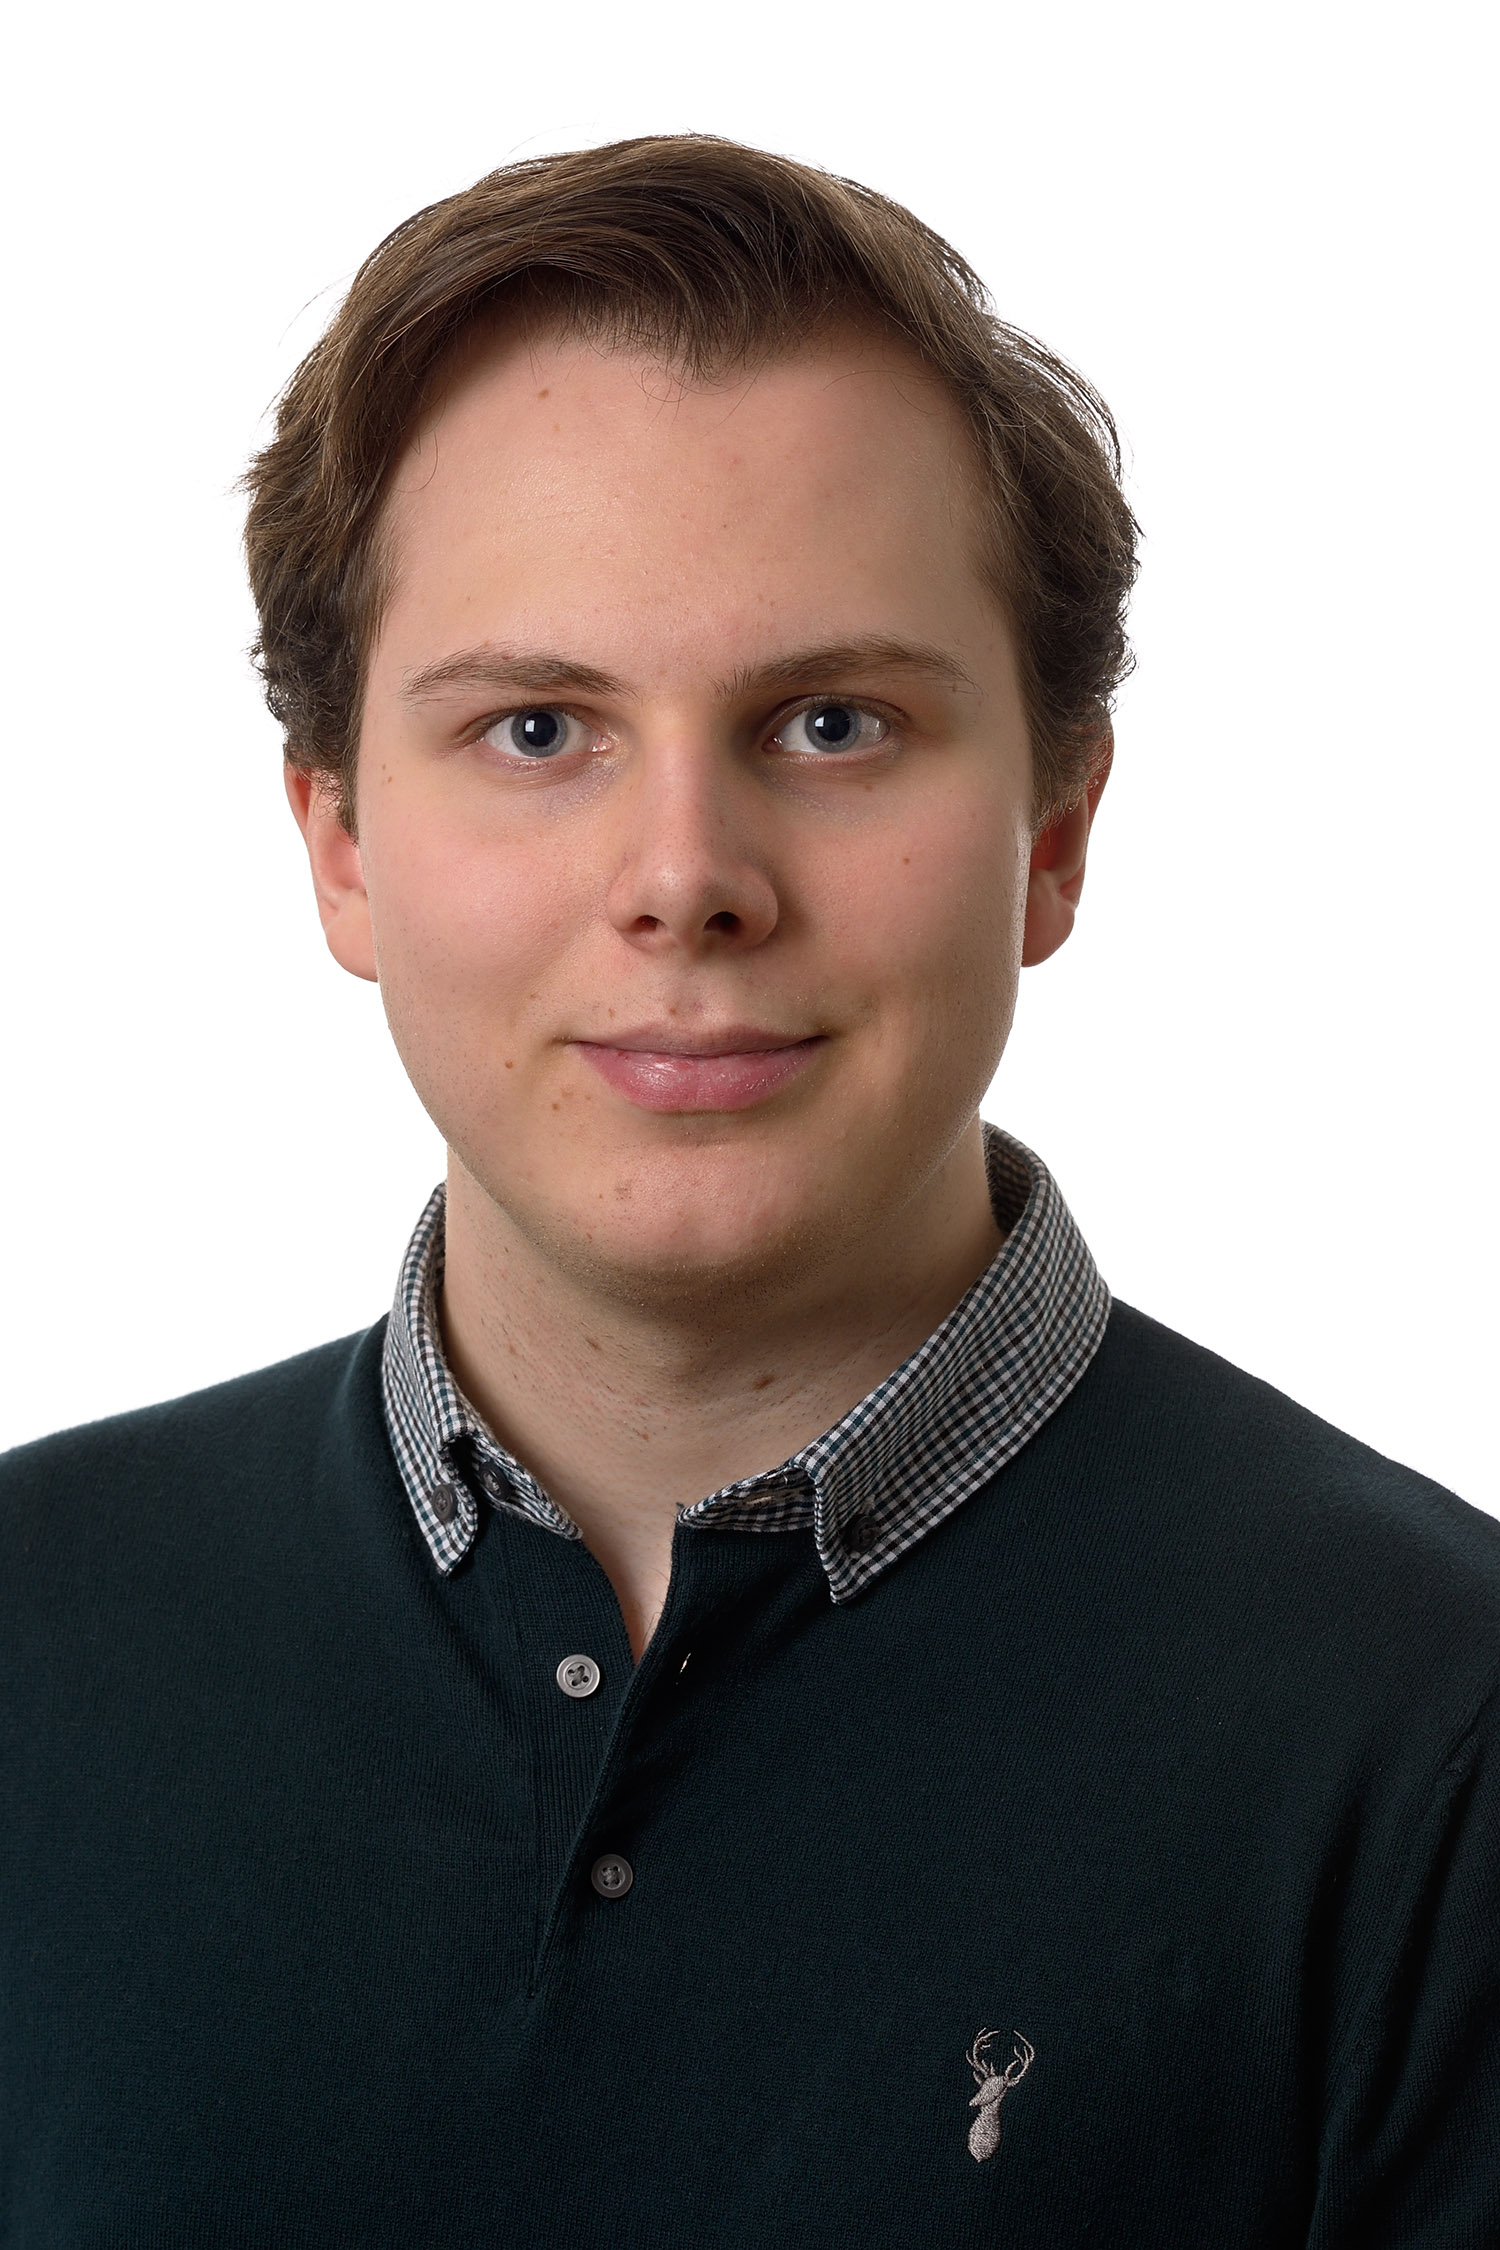
\includegraphics[width=0.2\textwidth]{0-cover/img/TEAMPICS/William_final.jpg}  & \textbf{William Eriksson - Software}

\smallskip
\textit{Current Education}: Master Programme in Space Engineering, Luleå University of Technology

\smallskip
\textit{Responsibilities}: Software (onboard \& ground station).
\bigskip
\\

\includegraphics[width=0.2\textwidth]{0-cover/img/TEAMPICS/Jon_final.jpg} & \textbf{Jon Mihkkal Inga - Mechanical}

\smallskip
\textit{Current Education}: Master Programme in Space Engineering, Luleå University of Technology

\smallskip
\textit{Responsibilities}: Mechanical (Structures and materials)

\label{tab:people}
\end{longtable}
\raggedbottom



\pagebreak
\section{Experiment Requirements and Constraints}
A list of requirements and constraints are listed below. The requirements are separated in functional, performance, design and operational requirements. %For a complete list of requirements that include obsolete ones, refer to Appendix \ref{sec:appFullListOfRequirements}.

\subsection{Functional Requirements}

\begin{enumerate}[topsep=0pt,itemsep=-0.5ex,partopsep=1ex,parsep=1ex]
    \item[F.1] \st{The telescope shall successfully track the celestial objects of interest.}
    \item[F.2] \st{The camera shall take images in the near infrared (NIR) spectrum.}
    \item[F.3] \colorbox{yellow}{\parbox{\textwidth}{The system shall be able to find the celestial objects of interest at the location and orientation of the gondola.}}
    \item[F.4] \colorbox{yellow}{\parbox{\textwidth}{The system shall be able to orient towards selected celestial objects of interest.}}
    \item[F.5] \colorbox{yellow}{\parbox{\textwidth}{The system shall be able to counter balance perturbations of the gondola during exposure.}}
    \item[F.6] \colorbox{yellow}{\parbox{\textwidth}{The camera and optics system shall be able to record the selected celestial object of interest.}}
\end{enumerate}

\subsection{Performance Requirements}

\begin{enumerate}
    \item[P.1] The gimbal stabilization system shall point the telescope towards the celestial object with an accuracy of at least 1 arcsecond.
    \item[P.2] The optics shall be capable of taking pictures of 0.5-1.5 x 0.3-1\,degrees.
    \item[P.3] The NIR camera shall make images in the range of 720-850 to 1200\,nm.
    \item[P.4] The NIR camera shall have a resolution of at least 16\,MP.
    \item[P.5] The NIR camera shall be able to make images with exposure times between 0.5 and 150\,seconds.
    \item[P.6] The experiment shall measure the location and orientation of the gondola.
\end{enumerate}
\newpage
\subsection{Design Requirements}

\begin{enumerate}[topsep=0pt,itemsep=-1ex,partopsep=1ex,parsep=1ex]
	\item[D.01] The experiment shall be able to operate in the temperature profile of the BEXUS environment.
	\item[D.02] The experiment shall be able to operate in the pressure profile of the BEXUS environment.
    \item[D.03] The experiment shall be able to operate in the vibration profile of the BEXUS environment.
    \item[D.04] \colorbox{yellow}{\parbox{\textwidth}{\st{The absolute orientation of the telescope relative to the gondola shall be known with a accuracy of 0.1\,degrees.} \textit{Moved to reg. P.8}}}
	\item[D.05] The supporting structure shall not twist by more than 0.1\,degrees.
	\item[D.06] \colorbox{yellow}{\parbox{\textwidth}{\st{The telescope shall not be pointed within 27\,degrees of the sun.} \textit{Moved to req. O.3}}}
	\item[D.07] The experiment shall be able to fly during day and night.
	\item[D.08] \colorbox{yellow}{\parbox{\textwidth}{\st{The temperature of the NIR camera shall be held at 0\,$\pm$5\,$^\circ$C.} \textit{Moved to req. P.11}}}
	\item[D.09] \colorbox{yellow}{\parbox{\textwidth}{\st{The images obtained shall be sent to a ground station by the E-link system with a maximum data rate of 1000\,kilo bits per second.} \textit{Moved to D.18}}}
	\item[D.10] The experiment shall be mounted at the side of the gondola.
	\item[D.11] The experiment shall not consume more power than 250\,Wh.
    \item[D.12] \colorbox{yellow}{\parbox{\textwidth}{\st{The volume of the experiment shall not exceed }\SI{0.11}{cm\cubed}.}}
    \item[D.13] The mass of the experiment shall not exceed 20\,kg.
    \item[D.14] The experiment shall be able to run for at least 2.5\,hours.
    \item [D.15] The experiment should be able to run for at least 4 hours
    \item[D.16] The experiment shall be able to function autonomously.
    \item[D.17] \colorbox{yellow}{\parbox{\textwidth}{The data stored in the experiment shall be able to survive the landing.}}
    \item[D.18] \colorbox{yellow}{\parbox{\textwidth}{The images obtained shall be sent to a ground station by the E-link system with a various and adjustable datarate between 250 and 1000 kilo bits per second.}}
\end{enumerate}

\subsection{Operational Requirements}

\begin{enumerate}[topsep=0pt,itemsep=-1ex,partopsep=1ex,parsep=1ex]
    \item[O.1] The experiment shall be able to be controlled by the ground station when requested.
    \item[O.2] The experiment shall rotate to a 'safe' location during ascent and descent.
    \item[O.3] \colorbox{yellow}{\parbox{\textwidth}{The telescope shall not be pointed within 27\,degrees of the sun.}}
\end{enumerate}
\subsection{Constraints}

\begin{enumerate}[topsep=0pt,itemsep=-1ex,partopsep=1ex,parsep=1ex]
    \item[C.1] \colorbox{yellow}{\parbox{\textwidth}{\st{The shared E-link data transfer rates are limited by coverage and quality of reception.}}}
    \item[C.2] \colorbox{yellow}{\parbox{\textwidth}{\st{There shall be no direct internet connection on the ground station.}}}
    \item[C.3] \colorbox{yellow}{\parbox{\textwidth}{\st{The mass and volume should fit inside the gondola together with the other experiments.}}}
    \item[C.4] \colorbox{yellow}{\parbox{\textwidth}{\st{The budget for the experiment is limited by the generous companies and organizations that sponsor IRISC.}}}
\end{enumerate}



\newpage
\section{Project Planning}

\subsection{Work Breakdown Structure}

\tikzset{
	basic/.style  = {draw, text width=2cm, font=\sffamily, rectangle},
	root/.style   = {basic, rounded corners=2pt, thin, align=center,
		fill=green!30},
	level 2/.style = {basic,sibling distance=15mm, rounded corners=6pt, thin,align=center, fill=green!60,
		text width=6em},
	level 3/.style = {basic, thin, align=left, fill=red!40, text width=6.5em},
	level 4/.style = {basic, thin, align=left, fill=red!20, text width=8em}
}

\begin{tikzpicture}[grow=right, , anchor=west, growth parent anchor=east, parent anchor=east, scale=\textwidth/15cm,
level 1/.style={sibling distance=35mm}, edge from parent/.style={->,draw},
>=stealth]


% root of the the initial tree, level 1
\node[root] {IRISC}
% The first level, as children of the initial tree
child {node[level 2] (c1) {Management}
	child{node[level 3] (c11){Project \\ Manager}
		child{node[level 4](c111){Diego Talavera}}
		}
	child{node[level 3] (c12){Outreach}
		child{node[level 4](c121){Veronika Haberle}}
		}
	}
child {node[level 2] (c2) {Science}
	child {node [level 3] (c21) {Astronomy}
		child{node[level 4](c211){Kim Steele}}
		}
	child {node [level 3] (c22) {Data Analysis}
		child{node[level 4](c221){Kim Steele \\ Veronika Haberle}}
		}
	}
child {node[level 2] (c3) {Mechanical}
	child {node [level 3](c31) {Thermal \\ Engineering}
		child{node[level 4](c311){Jack Hooper}}
		}
	child {node [level 3](c32) {Structures and Materials}
		child{node[level 4](c321){Ajith Kumar}}
		}
	}
child {node[level 2] (c4) {Electrical}
	child {node [level 3] (c41) {Embedded systems}
		child{node[level 4](c411){Elrick Weterings}}
		}
	child {node [level 3] (c42) {Energy \\ Technologies}
		child{node[level 4](c421){Sabina Bj{\"o}rk}}
		}
	}
child {node[level 2] (c5) {Software}
	child {node [level 3] (c51) {Control \\ System}
		child{node[level 4](c511){Anja M{\"o}slinger \\ Adam Smialek}}
		}
	child {node [level 3] (c52) {Onboard data}
		child{node[level 4](c521){Harald Magnusson \\ William Eriksson}}
		}
	child {node [level 3] (c53) {Ground station systems}
		child{node[level 4](c531){Niklas Ulfvarson}}
		}
	};


\end{tikzpicture}


The IRISC team is divided into 5 major branches: Management, Science, Mechanical Engineering, Electrical Engineering an Software Engineering. Diego Talavera will also work in the Mechanical Engineering branch whenever needed. The Electrical and Software Engineering branches will work closely together to achieve smooth integration between hardware and software.


\subsection{Schedule}

\begin{ganttchart}[
	hgrid,
	vgrid,
	expand chart=\textwidth,
	time slot format=isodate-yearmonth,
	time slot unit=month,
	]{2018-12}{2019-12}
	\gantttitle{BEXUS - IRISC}{13}\\
	\gantttitlecalendar{year, month=shortname} \\
	\ganttbar{Design Phase}{2018-12}{2019-04}\\
	\ganttbar{Unit testing}{2019-03}{2019-05}\\
	\ganttbar{Manufacturing Phase}{2019-04}{2019-07}\\
	\ganttmilestone {First Prototype}{2019-04}\\
	\ganttbar{Complete System Testing}{2019-06}{2019-09}\\
	\ganttbar{Launch Campaign}{2019-10}{2019-10}\\
	\ganttbar{Data Analysis Phase}{2019-11}{2019-12}
\end{ganttchart}

\subsubsection{Manpower}

This section will address the outline for the current available manpower of the IRISC team, this includes the tasks assigned to each member and the hours per week that each team member will dedicate to the project.

\begin{longtable}{m{0.25\textwidth} | m{0.6\textwidth} | m{0.1\textwidth}}
	\textbf{Team Member} & \textbf{Tasks Description} & \textbf{hours/week} \\ \hline
	Diego Talavera  & \textbf{Team Manager}. Was in charge of the management of the resources of the team and supervising the overall progress of the activities. Also provided technical support to the Mechanical Engineering branch. &  30-40 \\ \hline
	Niklas Ulfvarson & \textbf{ Vice Team Manager \& Ground Station System \& Star Tracker}. Was in charge of developing the software needed for monitoring and controlling (if needed) the experiment from the ground as well as to visualize the data received by the telemetry system. Also implemented the star tracker for attitude determination, and assisted with management and supervision of the team. & 30 \\ \hline
	Kimberly Steele & \textbf{Astronomy \& Data analysis}. Was in charge of the target selection and provide the technical requirements to achieve proper imaging of said targets. Was also involved in the data analysis after the BEXUS flight campaign and as well minor tasks for the outreach campaign. & 30 \\ \hline
	Jack Hooper & \textbf{Thermal Engineering}. Was to ensure that the thermal requirements for the proper functioning of the experiment during the ascent, flight and descent phases were met. This included design and selection of active/passive heating and cooling where needed and recommendations regarding materials. & 25 \\ \hline
	Elrick Weterings & \textbf{Embedded systems}. Was in charge of the design and selection for the electronic components including sensors and motors used to stabilize the telescope. He was also in charge of designing the necessary printed circuit boards (PCBs). & 30 \\ \hline
	Sabina Bj{\"o}rk & \textbf{Energy Technologies}. Was to ensure that the power required was delivered to all the subsystems during all phases of the experiment. & 25-35 \\ \hline
	Anja M{\"o}slinger & \textbf{Control System}. Was responsible for the development and testing of the control loop necessary to stabilize the telescope to the required degree of accuracy. & 30 \\ \hline
	Adam Smialek & \textbf{Control system}.  Helped in the development of the control loop, including the code testing and implementation. He also helped with some tasks in the Outreach branch, like the fundraising campaign. & 20 \\ \hline
	Harald Magnusson & \textbf{Onboard data}. Was in charge of the development of the software necessary by the experiment in order to function correctly, including data processing, handling and delivery. & 30 \\ \hline
	William Eriksson & \textbf{Onboard data}. Was also involved in the development of the software required on board of the experiment, this also included data processing and handling, telemetry, etc. & 30 \\ \hline
	Jon Mihkkal Inga & \textbf{Mechanical Engineering}. Designed the mechanical setup of the experiment, including FEM analysis and its construction. & 20 \\ \hline

\end{longtable}

\newpage
\begin{landscape}
	\begin{figure}[H]
		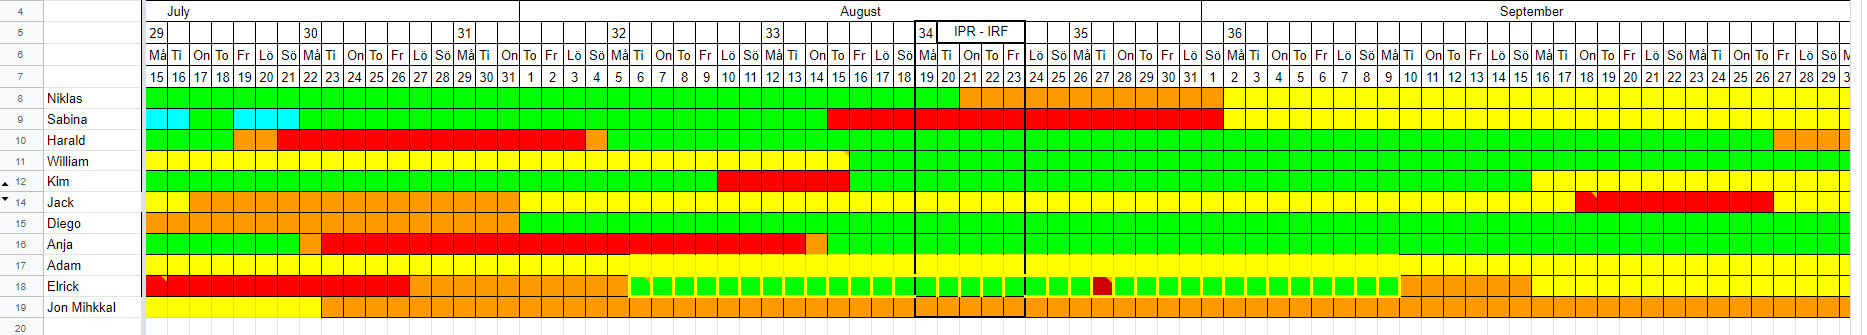
\includegraphics[scale=1.2]{3-project-planning/img/availability.png}
		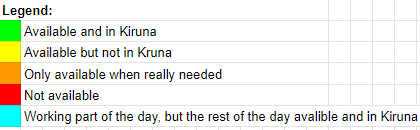
\includegraphics[scale=1.2]{3-project-planning/img/Availability_legend.png}
		\caption{Availability chart of the team members}
	\end{figure}
\end{landscape}

\newpage
\subsubsection{Budget}
\label{sec:3.2.2}

%This table is fancy and will line up your decimal points, unlike the normal table, so it looks prettier :3
\begin{table}[H]
\centering
\begin{tabular}{|l|c|c|c|} 
\hline
Source & Amount (\euro) & Limitations   \\ 
\hline
Luleå University of Technology & 1000 & Hardware and travel \\
SNSA & 3000 & Hardware and travel \\
Crowdfunding Campaign & TBD & None \\
\hline
\textbf{Total projected income} & \textbf{4000} & \\
\hline
\bf{Total projected cost} & \bf{2681.5} & \\
\hline
\end{tabular}
\caption{Income and projected cost.}
\label{table:income-and-cost}
\end{table}

\raggedbottom
%This table is fancy and will line up your decimal points, unlike the normal table, so it looks prettier :3
\begin{table}[H]
\centering
\begin{tabular}{|c|d{2}|d{2}|}%{D{.}{.}{1}}
\hline

\textbf{Category} & \textbf{Total Mass [g]} & \textbf{Total Price [EUR]} \\ \hline
Structure & 5000 & 500 \\ \hline
Electronics Box &  2000 & 500 \\ \hline
Telescope & 5000 & 1500 \\ \hline
Cables and Sensors &  &  \\ \hline
Tools & - & TBD \\ \hline
Travel & - & TBD \\ \hline
Contingency & - & TBD  \\ \hline
{\textbf{Total without Error Margin}} & \textbf{} & \textbf{TBD} \\ \hline
Shipping Costs and Error Margin &  &  \\ \hline
{\textbf{Total with Error Margin}} & \textbf{} & \textbf{TBD} \\ \hline
\end{tabular}
\caption{Mass and Cost Budget.}
\label{table:mass-and-cost-budget}
\end{table}

\raggedbottom


\subsubsection{External Support}

\begin{itemize}
	\item Mr. Olle Persson. Provided help with getting access to some testing facilities as well as potential questions in the Mechanical Engineering branch of the project.
	\item Adam Burgasser, PhD. Helped us with the data analysis and interpretation after the flight with BEXUS.
	\item LUDD - Luleå Academic Computer Society. They provided the hosting to the official IRISC web page.
	\item GranaSAT, team from Bexus 19 which provided help with the attitude determination system.
\end{itemize}



\subsection{Outreach Approach}
An important focus of the project is the topic of outreach. During the whole timeline, updates about the project will be shared with as many people as possible. The most effective way of reaching people is via social media. IRISC is represented on the following social media platforms:
\begin{itemize}
	\item facebook.com/IRISCBexus
	\item instagram/IRISC\_BEXUS
	\item twitter/IRISCBEXUS
\end{itemize}
Additionally to the social media platforms, the team's website with information about the project is available and updates are blogged there regularly.\newline\newline
Future outreach plans include, but are not limited to,:
\begin{itemize}
	\item articles at university blog of the Lule{\aa} University of Technology
	\item articles in local newspaper
	\item visibility through posters, flyers, etc at university
	\item presentations during local events
	\item applications to grants and awards
\end{itemize}

In addition to the above outreach goals, the team would like to coordinate community and school visits with the optical part of the experiment for astronomical observing with the general public. With a solar filter, the telescope would be capable of observing the sun, and with the appropriate lenses would be capable of observing the moon and other popular objects, such as the planets, in dark sky conditions. Public astronomy opportunities not only fuel public interest in space, science and engineering, but would give the team the opportunity to raise awareness of the IRISC project and the REXUS/BEXUS project as a whole.\\
Contact has been made with the local "space high school" (\textit{Rymdhuset}) here in Kiruna, Northern Sweden, to gauge interest in involvement with the project, with the intention of giving a talk about the project to prospective space science students in the local community. 
\pagebreak
\subsection{Risk Register}
\textbf{Risk ID}
\begin{enumerate}[label={}]
    \item TC – Technical/Implementation 
    \item MS – Mission (operational performance) 
    \item SF – Safety 
    \item VE – Vehicle 
    \item PE – Personnel 
    \item EN – Environmental 
    \item OR - Outreach
    \item BG - Budget
\end{enumerate}

Adapt these to the experiment and add other categories. 
Consider risks to the experiment, to the vehicle and to personnel. 

\textbf{Probability (P)}
\begin{enumerate}[label=\Alph*]
    \item Minimum – Almost impossible to occur 
    \item Low – Small chance to occur 
    \item Medium – Reasonable chance to occur 
    \item High – Quite likely to occur 
    \item Maximum – Certain to occur, maybe more than once
\end{enumerate}

\textbf{Severity (S)}
\begin{enumerate}
    \item Negligible – Minimal or no impact 
    \item Significant – Leads to reduced experiment performance 
    \item Major – Leads to failure of subsystem or loss of flight data 
    \item Critical – Leads to experiment failure or creates minor health hazards 
    \item Catastrophic – Leads to termination of the REXUS/BEXUS programme, damage to the vehicle or injury to personnel 
\end{enumerate}

The rankings for probability (P) and severity (S) are combined to assess the overall risk classification, ranging from very low to very high and being coloured green, yellow, orange or red according to the SED guidelines.

Whether a risk is acceptable or unacceptable has been assigned according to the SED guidelines. Where mitigation is written for acceptable risks this details the mitigation undertaken in order to reduce the risk to an acceptable level.

\begin{landscape}
% highy recommend https://www.tablesgenerator.com/


\begin{longtable}{|m{0.075\textwidth}| m{0.48\textwidth} |m{0.02\textwidth} |m{0.02\textwidth}|m{0.10\textwidth}| m{0.64\textwidth}|}

\hline
\textbf{ID} & \textbf{Risk (\& consequence if)} & \textbf{P} & \textbf{S} & \textbf{P * S} & \textbf{Action} \\ \hline


TC10 & Optics and/ or camera destroyed due to testing						& C & 2 & \cellcolor[HTML]{FCFF2F}Low 		& There is budget for a spare part, it is quite easy to get and test where it will likely fail (e.g. drop test) will not be done with this part.\\\hline

TC20 & Optics and/ or camera destroyed due to looking directly into the sun & B & 3 & \cellcolor[HTML]{FCFF2F}Low 		& A model will be made and \hl{thorough testing will be made to mitigate this risk. The control system will also ensure to avoid looking into the sun }.\\\hline

TC30 & Software failure														& B & 3 & \cellcolor[HTML]{FCFF2F}Low 		& A watchdog with power-on-reset will be added to the design.\\\hline

TC40 & Motors of the gimbal are uncontrollable								& B & 4 & \cellcolor[HTML]{FCFF2F}Low 		& It will be made sure that a single component failure will not result in this consequence.\\\hline

TC50 & Motors overloaded													& A & 3 & \cellcolor[HTML]{34FF34}Very Low 	& Sufficient testing and modeling will be done to decrease the probability.\hl{Safety measures will be added to the power system to prevent overloading}\\\hline

TC60 & PCB failure \hl{due to defective traces or component}												& B & 3 & \cellcolor[HTML]{FCFF2F}Low 		& \st{sufficient} Testing will be performed on each PCB to decrease the probability.\\\hline

TC70 & Single component failure gives unprecedented failure					& B & 4 & \cellcolor[HTML]{FCFF2F}Low			& A Failure mode and effects analysis (FMEA) study will be done so that single failure components with a high impact will be documented and migrated.\\\hline

TC80& Moving parts jamming \hl{due to moisture freezing}& B & 3 & \cellcolor[HTML]{FCFF2F} Low & Moving parts will be \st{properly} cleaned and lubricated where needed. \\\hline
\hl{TC90} & \hl{The structure is not stiff enough} & \hl{A} & \hl{2} & \cellcolor[HTML]{34FF34}Very Low & \hl{FEM analysis and testing will performed to ensure the necessary stiffness is achieved.} \\ \hline

\hl{TC90} & \hl{Values for R and Q matrices of PID controller not chosen correctly for Kalman filter} & \hl{B} & \hl{2} & \cellcolor[HTML]{FCFF2F}Low	& \hl{Thorough analysis, simulations and testing will be conducted to tune the tuned correctly.} \\ \hline

MS10 & Target not found	& D & 2 & \cellcolor[HTML]{FCFF2F}Low			& The ground station will be able to correct this, or send the system to another target.\\\hline

MS20 & Damage to the system on landing										& D & 1 & \cellcolor[HTML]{FCFF2F}Low			& Optics will rotate into a position where damage can be avoided/minimized.\\\hline

MS30 & Damage to the storage unit on landing									& C & 2 & \cellcolor[HTML]{FCFF2F}Low			& Data will be send over telemetry\\\hline

MS40 & Storage unit full during flight											& A & 3 & \cellcolor[HTML]{34FF34}Very Low	& \hl{The data handling system will be thoroughly tested, and the storage unit(s) will be of more capacity than it is expectede to use} \st{modeling will be done to decrease the probability}.\\\hline

MS50 & BEXUS balloon power failure											& A & 4 & \cellcolor[HTML]{34FF34}Very Low	& -\\\hline

MS60 & BEXUS balloon telemetry failure										& B & 2 & \cellcolor[HTML]{34FF34}Very Low	& The system will be able to function autonomously.\\\hline

MS70 & Critical electronic components overheating & B & 3 & \cellcolor[HTML]{34FF34}Very Low & Peltier elements and heat sinks will be added where necessary. \\\hline

MS80 & Scientific objective not achieved & B & 3 & \cellcolor[HTML]{FCFF2F} Low & \hl{Systems will be designed so that scientifically relevant data will be obtained, for example, sensor fusion will be implemented to the gyroscope and star tracker to improve tracking accuracy.}\st{Critical components for the pointing system will be selected, designed and manufactured with a high enough safety factor.}\\\hline

SF10 & Components falling off the gondola									& A & 4 & \cellcolor[HTML]{34FF34}Very Low	& All parts \hl{securely} \st{sufficiently} fastened. Testing will be conducted to ensure the fastening is able to hold all parts in place \st{in case of turbulence}. Where deemed necessary, additional fixations will be added.\\\hline

VE10 & Short circuiting														& B & 3 & \cellcolor[HTML]{FCFF2F}Low			& A fuse is added in the power system.\\\hline

PE10 & Miscommunication in the team											& B & 2 & \cellcolor[HTML]{34FF34}Very Low	& The management team should be responsible for ensuring \hl{important} \st{proper} information is conveyed to all team members.\\\hline

PE20 & People are not available												& C & 1 & \cellcolor[HTML]{34FF34}Very Low	& An availability sheet is made so a planning can be made. This will be kept up to date during the entire project.\\\hline

PE30 & Management team unavailable to oversee project						& C & 1 & \cellcolor[HTML]{34FF34}Very Low	& There is always someone as a backup.\\\hline

PE40 & Sudden resignation of project members								& B & 2 & \cellcolor[HTML]{34FF34}Very Low	& Management team ensure morale remains high through a variety of techniques (team building activities).\\\hline

\hl{BG10} & \hl{Budget is not sufficient} & \hl{B} & \hl{4} & \cellcolor[HTML]{FCFF2F}Low & \hl{Management team will ensure that the budget is enough as well as keep in contact with companies and institutions for any possible support and/or sponsorship.} \\ \hline

\hl{BG20} & \hl{Schedule delays} & \hl{C} & \hl{2} & \cellcolor[HTML]{F39C12} Medium & \hl{Planning of critical dates will be done and made easily accessible for all the team members} \\ \hline



\caption{Risk Register.}
\label{tab:risk-register}
\end{longtable}
\raggedbottom
\end{landscape}

\pagebreak
\section{Experiment Design}
\subsection{Experiment Setup} \label{Experiment_Setup}

%\colorbox{orange}{\parbox{\textwidth}{I know this is more like the SUNBYTE structure and not so much like the EXIST one, but in this particular case I prefer the readability of SUNBYTE}}



%very general experiment setup
The experiments mounts a telescope with an attached CMOS sensor inside the gondola, looking out as shown in figure \ref{fig::4-1_CAD}. The telescope is mounted on a gimbal system that provides stabilisation along two axes (three if required, depending on simulation results, hardware is available) and tracking in three dimensions. The sensor/telescope/gimbal system will be shielded from the Sun's radiation and climatised in order to provide the required operation temperatures. This is achieved by using Peltier elements where heating or cooling may be necessary (e.\,g.~the sensor) and heating pads where there is only a chance of freezing (e.\,g.~the moving parts of the gimbal). The general setup with data flows can be seen in figure \ref{fig::4-1_block_diagram}. The individual sections of the experiment are described below.

\begin{figure}[h]
	\centering
	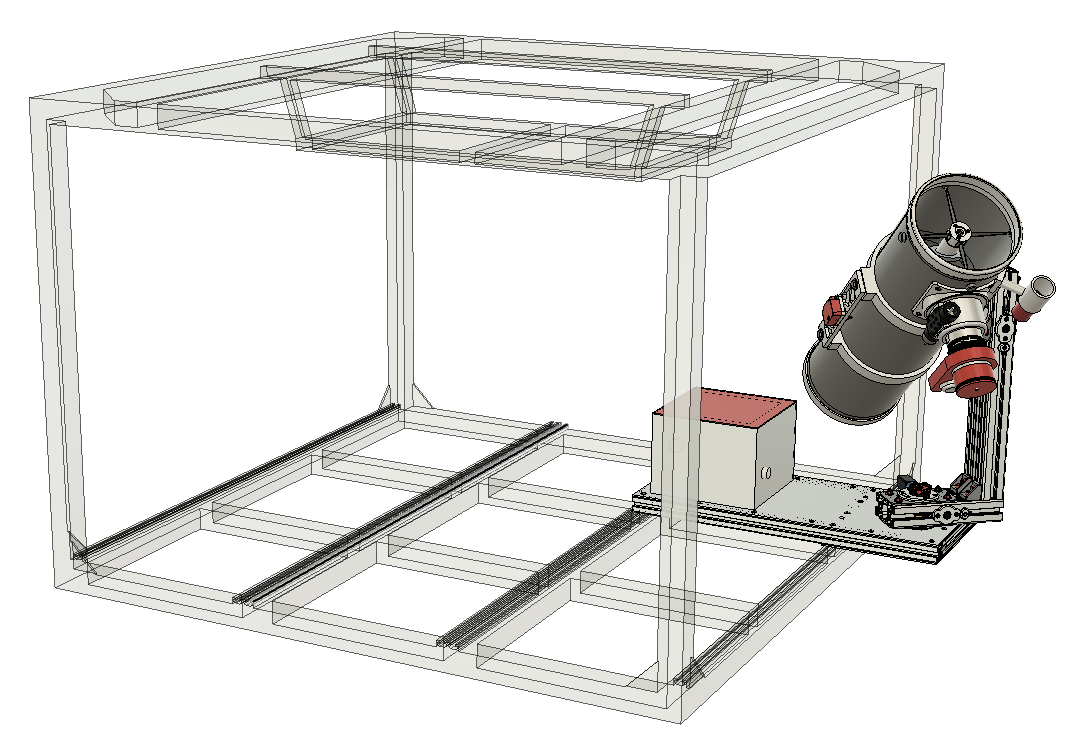
\includegraphics[width=0.7\linewidth]{4-experiment-design/img/mechanical/iso0.png}
	\caption{CAD-model of the experiment}
	\label{fig::4-1_CAD}
\end{figure}


\subsubsection{Telescope and CMOS sensor}
% telescope and CMOS sensor
The telescope chosen is a Sky-Watcher~BKP~130~DS (see figure \ref{fig::4.1-telescope}), a parabolic Newtonian reflector with a focal length of 650\,mm, an optical diameter of 130\,mm and therefore featuring an aperture ratio of $f/5$. 

The imaging sensor used is ZWO ASI183MM (mono) (see figure \ref{fig::4.1-sensor}), a CMOS sensor with only one channel (mono, not color) with a resolution of 20.18\,MP (5496x3672), a sensor size of 13.2x8.8\,mm (diagonal: 15.86\,mm) and a pixel size of 2.4x2.4\,$\mu$m. To limit the wavelength bandwidth imaged, an IR filter that filters out any wavelengths below 720\,nm is used in order to use the sensor as a NIR camera.

The imaging spectrum of the NIR imaging sensor is illustrated in figure \ref{fig::4.1-NIR_spectrum}.

\begin{figure}[h]
	\centering
	\begin{minipage}[t]{0.3\linewidth}
		\centering
		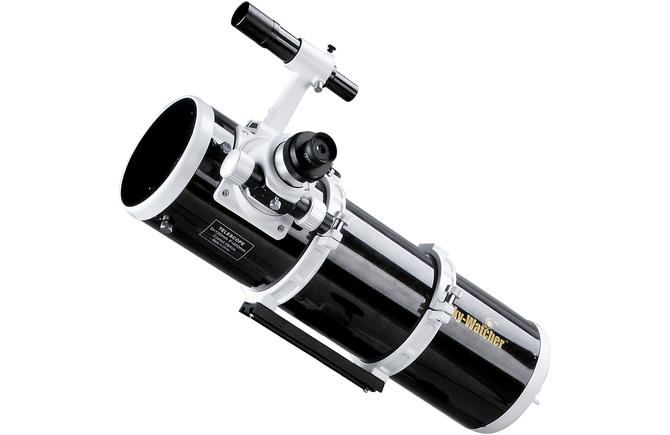
\includegraphics[width=1.0\linewidth]{4-experiment-design/img/setup/SkyWatcher_BKP130DS}
		\caption{Sky-Watcher BKP~130~DS}
		\label{fig::4.1-telescope}
	\end{minipage}
	%\hfill
	\hspace{0.03\linewidth}
	\begin{minipage}[t]{0.3\linewidth}
		\centering
		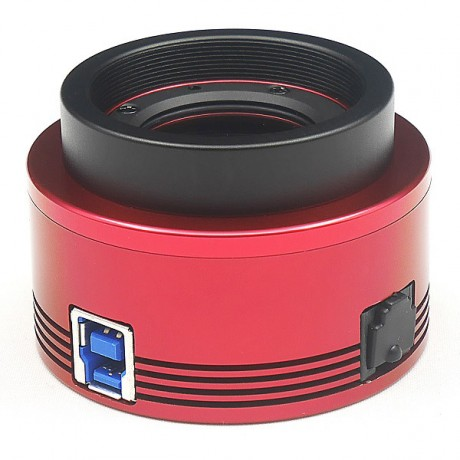
\includegraphics[width=0.65\linewidth]{4-experiment-design/img/setup/ZWO_ASI183MM}
		\caption{ZWO ASI183MM (mono) (NIR camera)}
		\label{fig::4.1-sensor}
	\end{minipage}
	\hspace{0.03\linewidth}
	\begin{minipage}[t]{0.3\linewidth}
		\centering
		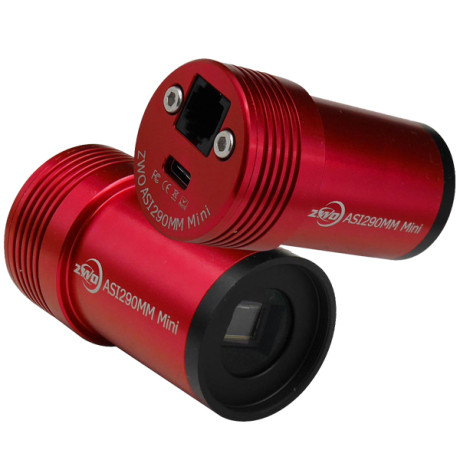
\includegraphics[width=0.7\linewidth]{4-experiment-design/img/setup/ZWO_ASI290MM_Mini}
		\caption{ZWO ASI290 Mini (mono) (guiding camera)}
		\label{fig::4.1-guiding_camera}
	\end{minipage}

\end{figure}

\begin{figure}[H]
	\centering
	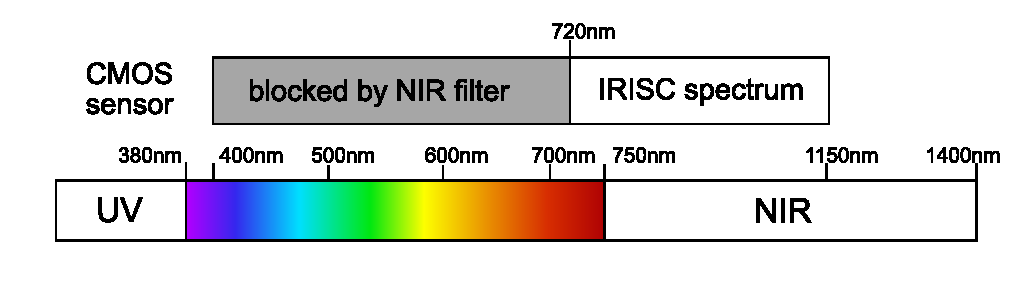
\includegraphics[width=0.8\linewidth]{4-experiment-design/img/setup/IRISC_spectrum}
	\caption{Imaging spectrum of the NIR camera}
	\label{fig::4.1-NIR_spectrum}
\end{figure}

\begin{figure}[H]
	\centering
	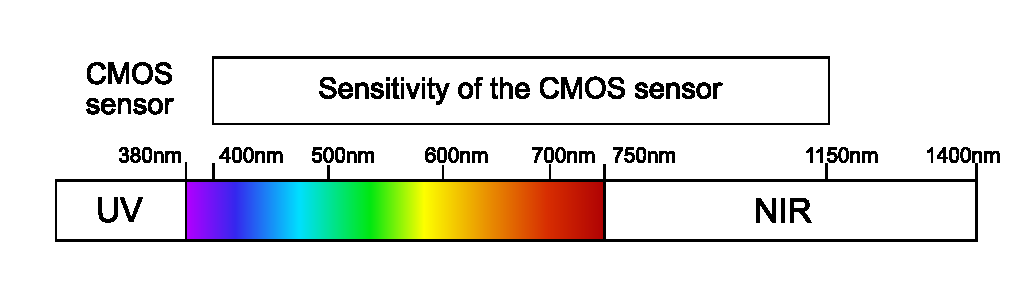
\includegraphics[width=0.8\linewidth]{4-experiment-design/img/setup/CMOS_spectrum}
	\caption{Imaging spectrum of the guiding camera}
	\label{fig::4.1-CMOS_spectrum}
\end{figure}

This combination of telescope and sensor features the following specifications:

\begin{itemize}
	\item \textbf{Field of View (FoV):} the field of view determines the astronomical targets that can be observed. It depends on the sensor size and the focal length of the telescope. Naturally, there is a horizontal, a vertical and a diagonal field of view:
	\begin{align}
		\text{FoV}_\text{horizontal} &= \arctan \frac{\SI{13.2}{mm}}{\SI{650}{mm}} = \ang{1,16} \\
		\text{FoV}_\text{vertical} &= \arctan \frac{\SI{8.8}{mm}}{\SI{650}{mm}} = \ang{0,757} \\
		\text{FoV}_\text{diagonal} &= \arctan \frac{\SI{15,86}{mm}}{\SI{650}{mm}} = \ang{1,382}
	\end{align}
	\item \textbf{Sensor resolution:} the angular resolution per pixel defines the precision of the scientific data collected.
	\begin{align}
		\text{Resolution} = \arctan \frac{\SI{2,4}{\um}}{\SI{650}{mm}} %= \SI{2,1155e-4}{\degree}
		 = \ang{;;0,7616}
	\end{align}
\end{itemize}

In order to examine the field of view in case the images sent down via downlink do not show the expected astronomical targets, an additional imaging sensor (ZWO ASI 290MM Mini) is installed on a guiding telescope that has a shorter focal length than the main telescope, implying a larger field of view (see figure \ref{fig::4.1-guiding_camera}). This sensor has the same sensitivity spectrum as the NIR camera, but it is not intended to block out any of the visible or NIR wavelengths in order to maximise the incident light and therefore the input signal. The spectrum is illustrated in figure \ref{fig::4.1-CMOS_spectrum}. With the help of these pictures it will be able to correct offset errors in the pointing mechanism of the control system due to e.\,g.~temperature drift of the sensors. In addition to this a small sanity camera with a wide angle lens (very large field of view) to keep track of the system status and detect possible errors if neither the NIR images nor the images from the guiding telescope show the expected results may be installed (not included in figures \ref{fig::4-1_CAD} and \ref{fig::4-1_block_diagram}).



\subsubsection{Electronics}

\begin{figure}[htb]
	\centering
	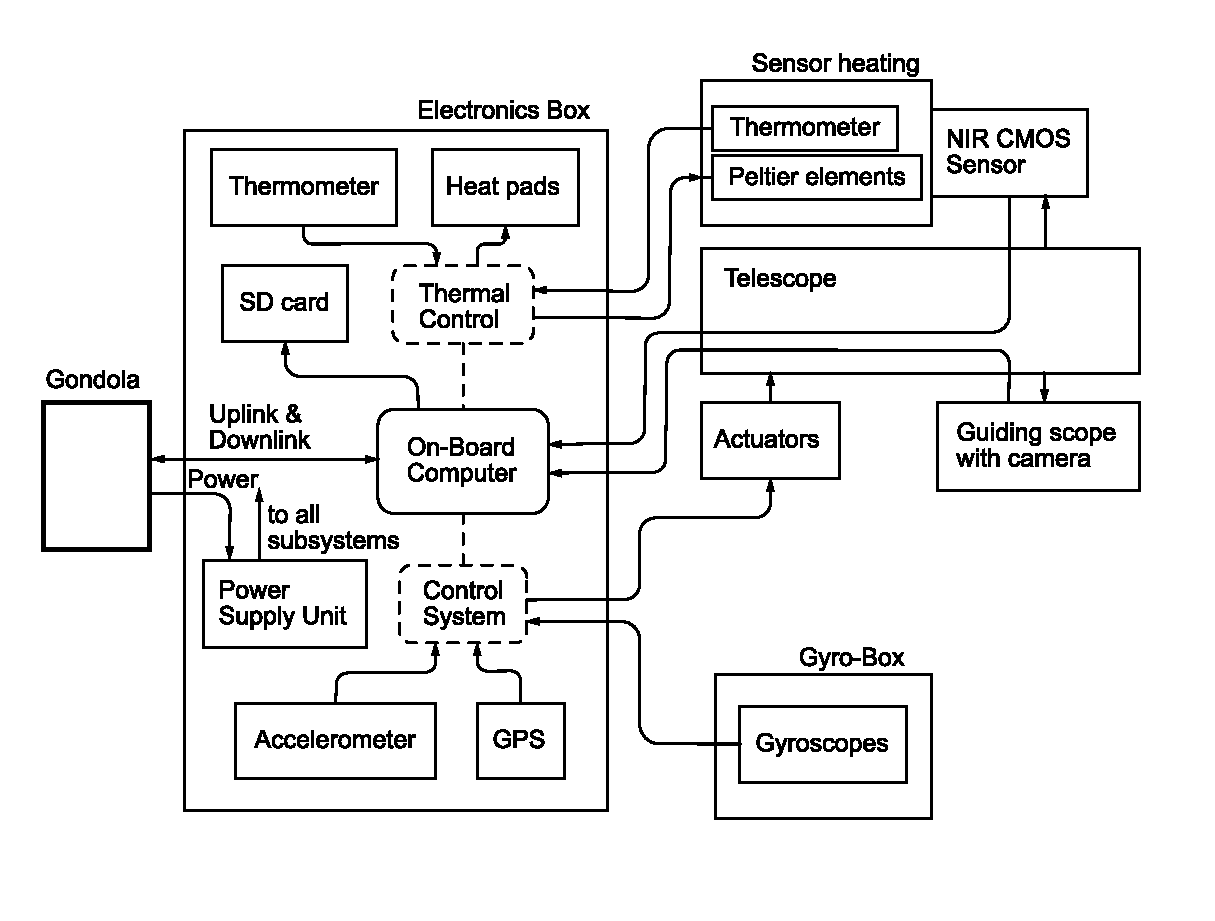
\includegraphics[width = \linewidth]{4-experiment-design/img/setup/Block_diagram_4-1}
	\caption{Block diagram of the experiment setup}
	\label{fig::4-1_block_diagram}
\end{figure}

% content of electronics box
The On-Board Computer is hosted by the electronics box that also features the onboard storage as well as the power supply unit, one set of gyroscopes and accelerometers to measure the movement of the gondola in order to provide input data to the control system, a GPS (for the control system), temperature sensors for housekeeping data and the heat management system inside the electronics box and heating elements. The sensors are located on a PCB designed by the electronics team, along with the power supply unit. In order to minimise disturbances by the power electronics and actuators, the gyroscopes are housed by a separate gyro-box that is shielded by a metal housing.



% data storage, electronics box
The CMOS sensor data is transmitted to the On-Board Computer where it is compressed with lossless compression and sent down via E-link and is also stored onboard the BEXUS balloon. The onboard storage is located in the electronics box that is designed considering compatibility with the harsh environmental conditions as well as redundancy. The mechanical structure that features the onboard storage ensures survival in case of shock due to hard impact when landing or if the BEXUS balloon lands in a lake or wetlands.

% thermal shielding - required?

\subsubsection{Control system}
% control system and actuation
The control system is responsible for tracking the target in the sky and stabilising the telescope during exposure. The tracking uses the current orientation of the gondola along the z-axis measured by a magnetometer as well as the orientation of the telescope within the gondola using encoders. Based on the current time and position (measured by the GPS system) as well as the operational field of view, the control system will select and track the target in order to point the telescope towards the astronomical targets and avoid star trails due to the sky's rotation as seen from an observer on Earth. The stabilisation system is responsible for keeping the telescope steady during exposure by counteracting the gondola movements measured by the gyrometers and accelerometers located on the sensor PCB in the electronics box.


\subsubsection{Attitude determination}
In order to determine the attitude of the gondola as it is rotating, the guiding camera will also function as a star tracker. As the relative orientation of the telescope with respect to the gondola is known, the gondola attitude can be calculated and used for the control system. The star tracker will be based on the system used by team GranaSAT which flew on Bexus 19. Their experiment was able to correctly identify 445 star fields and incorrectly identified 10. Several images had to be discarded due to a lack of found stars, but as their camera also acted as a horizon detector the FOV of stars was limited. As their software worked well and was run on-board on a Raspberry Pi the conditions are generally similar. Contact is established with members from team GranaSAT, and with their support the star tracker software will be adapted for IRISC. It should be noted that GranaSAT flew during night time, while IRISC will most likely be flying during day time. However, as the tracker will be used above the atmosphere it should be able to producer similar results anyway.

Another system that has been shown to work under similar conditions is the Daystar Star Tracker \cite{daystar}. It was flown during daytime on a NASA balloon, piggybacking on a test of the WASP system. It was shown that daytime star tracking is possible with good results. Some of the modifications that had to be applied was a high pass filter to remove any Rayleigh scattering, and efficient star identification algorithms. Also, some extra image processing was needed. As their project was well documented, and all their software is open source, this too will be used to aid the development of the star tracker for IRISC.

\hl{After some consideration and testing, the star tracker used will be a slightly modified version of the Tetra algorithm developed by Julian Brown of MIT. This algorithm was chosen based on it being both calibrationless and very fast for the lost-in-space problem \mbox{\cite{tetra}}. Small adjustments and tuning is done in order to maximize performance for the specific use case of IRISC.}

\hl{One of the main changes was the catalogue used by the algorithm. Originally, Tetra is made to use the Yale Bright Star Catalogue, with a total of 9110 stars. This works for a FoV greater than 10 degrees, as the algorithm needs at least 10 stars to resolve the attitude. This however does not fit the IRISC use case, as the FoV of the guiding scope will be approximately 2.3 $\deg$ along the diagonal, resulting in about 4 sqare degrees. Instead, the algorithm is given the Hipparcos-2 catalogue, with a total of 117955 stars, and an average density of 3 stars per square degree. As such, an image from the guiding scope will include approximately 12 indexed stars, which is enough to find the attitude. The larger catalogue size increases the time to generate hash tables and such exponentially, but the time to resolve an image should not increase substantially.}



%\colorbox{red}{currently not included: guiding scope \& camera -> needs to be included!}













































\raggedbottom

\pagebreak
\subsection{Experiment Interfaces}

\subsubsection{Mechanical Interfaces}
\label{sec:4.2.1}

%\colorbox{orange}{\parbox{\textwidth}{THIS SECTION WILL BE FINALISED WHEN AN UPDATED CAD MODEL AND INTERFACE DESIGN WILL BE AVAILABLE}}\\

The experiment mounting platform will be attached to the lower rails of the gondola.

% Discuss mounting safety


\begin{figure}[H]
    \centering
	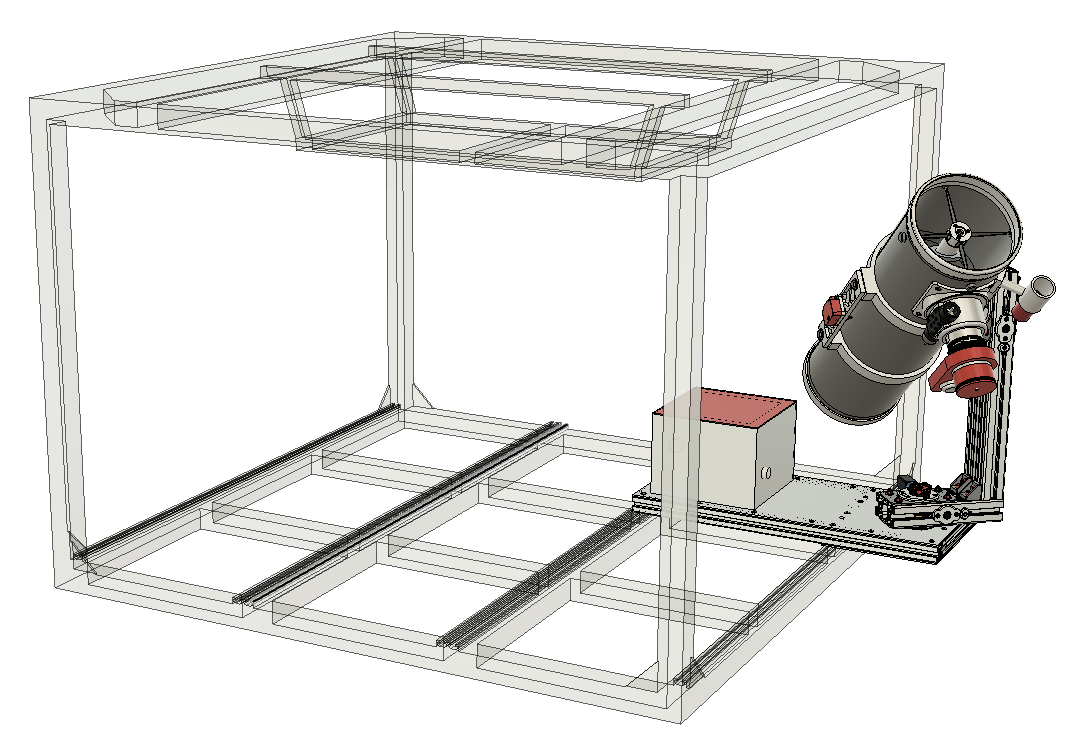
\includegraphics[width=0.9\linewidth]{4-experiment-design/img/mechanical/iso0.png}
	\caption{Instrument position on gondola}
\end{figure}


% \bigskip
% \input{4-experiment-design/tables/attaching_comp.tex}


\subsubsection{Thermal Interfaces}

%\colorbox{orange}{\parbox{\textwidth}{THIS SECTION REQUIRES THERMAL ANALYSIS AND DESIGN}}\\

The IRISC experiment will be shielded from heat sources that could potentially introduce noise to the measurements. Once the final selection of components is made, Finite Element Analysis will be used to optimize the configuration of the components to ensure a good system performance.

\label{sec:4.2.2}


\subsubsection{Electrical Interfaces}
\label{sec:4.2.3}
\textbf{E-link:}\\
The uplink will be used to send occasional commands to control the experiment. The downlink will be used to send science and housekeeping data to the ground station. The TCP/IP protocol will be used for both the uplink and the downlink. The communication overhead for the uplink and downlink are composed of the TCP header (maximum 480 bits), the IP header (maximum 480 bits) and the Ethernet frame (144 bits). This results in an overhead of roughly 5 to 10\,\%. The size of one command will at most be in the single digit kB range resulting in a maximum uplink bandwidth of 1\,kbit/s. The downlink is greater in size due to scientific data with a minimum bandwidth of 300\,kbit/s and a nominal bandwidth of 500\,kbit/s. See paragraphs "Interfaces" and "Data acquisition and storage" in section \ref{sec:4.8.2} for more detail regarding the downlink.

\textbf{Power:}\\

Placed on the outside of the experiment structure/housing, the experiment will have a 4 pin, male, box mount receptacle MIL–C-26482P series 1 connector with an 8-4 insert arrangement (MS3112E8-4P).


% I comment this out because of Tomas comment that poower in not an interface. Also removed the 1mA. 
% Power will be delivered to the electronics box from the provided 28.8 V (13 Ah) battery pack. Only one pack is required. The expected % minimum current is [\hl{TBD}], the average is [\hl{TBD}] and the maximum is [\hl{TBD}]. More details in \ref{sec:4.7}.

\textbf{Connectors:}\\

%\begin{figure}[H]
%    \centering
%	\includegraphics[width=0.2\linewidth]{4-experiment-design/img/interfaces/power_cables.jpg}
%	\caption{[\hl{PLACEHOLDER}] Position of power cable socket}
%	\label{fig:power_cables}
%\end{figure}
%
%\begin{figure}[H]
%    \centering
%	\includegraphics[width=0.2\linewidth]{4-experiment-design/img/interfaces/elink_cables.jpg}
%	\caption{[\hl{PLACEHOLDER}] Position of E-link cable socket}
%	\label{fig:elink_cables}
%\end{figure}

Info about power cables, their length/resistivity and thus power loss, their connection to gondola power relay.



\textbf{Connectors:}\\

\textbf{Protection:}\\

\textbf{Grounding:}\\


\subsubsection{Radio Frequencies (Optional)}



\raggedbottom

\begin{landscape}
\subsection{Experiment Components} \label{components}
\label{sec:experiment-components}

\subsubsection{Electrical Components}

% Table \ref{tab:components-table-electrical} shows all required electrical components with their total mass and price.\\

% \input{4-experiment-design/tables/component-table-electronics.tex}

\end{landscape}

\begin{landscape}

\subsubsection{Mechanical Components}

% Table \ref{tab:components-table-mechanical} shows all required mechanical components with their total mass and price.\\


% \input{4-experiment-design/tables/component-table-mechanical.tex}

\raggedbottom
\end{landscape}

\begin{landscape}
\subsubsection{Other Components}
% Table \ref{tab:component-table-other} shows other components which contribute to the mass and/or price.\\

% \input{4-experiment-design/tables/component-table-other.tex}


\raggedbottom
\end{landscape}
\newpage
\subsection{Mechanical Design} \label{Mechanical_Design}
\label{sec:mechanical-design}

\subsubsection{Structure}
\label{sec:4.4.1}
The experiment itself has only two components that are placed inside the gondola. Firstly, the electronics box and then the gimbal on which the telescope is mounted. We require the gimbal to be placed at the edge of the gondola so that the telescope setup is stowed during launch and descent, but still capable of being deployed and performing its required range of motion for observing astronomical targets outside of the gondola.

\begin{figure}[H]
    \centering
	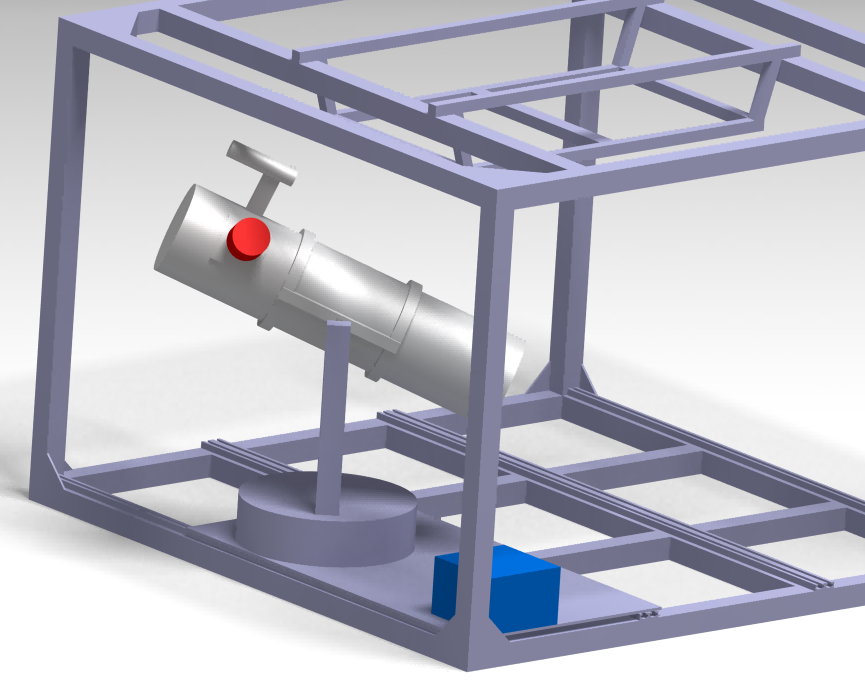
\includegraphics[scale=1.2]{4-experiment-design/img/mechanical/Assembly_3.png}
	\caption{Gimbal structure}
\end{figure}
\subsubsection{Electronics box}
\label{sec:4.4.2}
The electronics box has a dimension 10x10x10 cm which is placed directly inside the gondola. It is estimated to weigh 1.5 kg. The box is made of aluminium side plates with a thick layer of styrofoam placed on the inside of the aluminium plates which protects the electronics. The box has rubber cushion feet that acts as a shock absorber and also thermal insulator from the gondola.

\subsubsection{Gimbal}
\label {sec:4.4.3}
We intend to use a three axis gimbal so that we have a maximum field of view. We use CFRP to manufacture the gimbal. The gimbal along with telescope is estimated to weigh around 10kg.



\subsubsection{Fixing interface}
\label {sec:4.4.5}
The telescope itself has certain fixture points and as such, the gimbal will be designed with matching fixture points. The gimbal is directly fixed on the gondola. The gimbal along with the fixing points will first be tested with Finite Element Analysis (FEA) in order to ensure that the whole structure can withstand the loads indicated in the BEXUS manual. 

\pagebreak
\subsection{Electrical Design}
The electrical design provides the hardware required for the implementation of the software, the sensors for the control system and furthermore a communication interface to the BEXUS system. A global diagram with the electrical interfaces between the IRISC experiment and BEXUS balloon are shown in figure \ref{fig:elec-ACD}. %The main interfaces are the E-Link and the power. But also, the camera's/ telescope should be able to watch the sky from the gondola.}}
\vspace{-.5cm}
\begin{figure}[H]
	\centering
	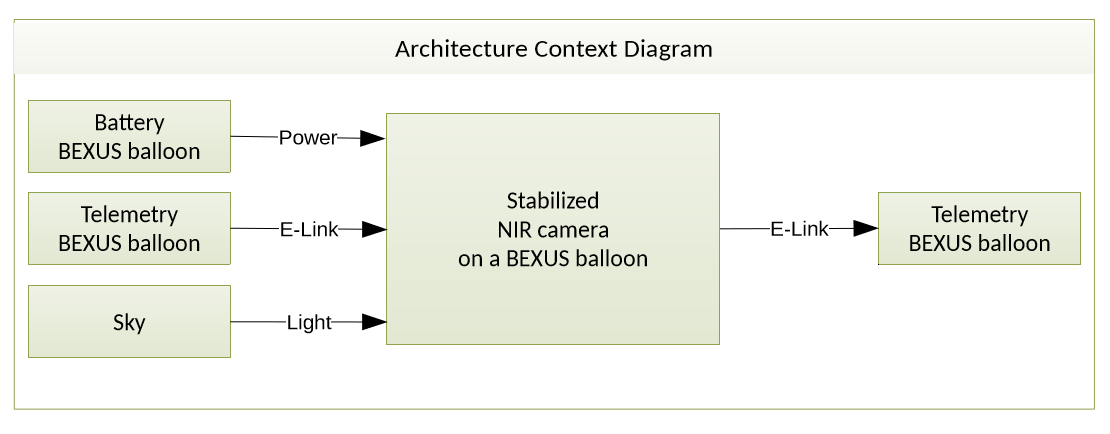
\includegraphics[width=.6\textwidth]{4-experiment-design/img/electrical/ArchitectureContext.png}
	\caption{Electrical architecture context diagram.}
	\label{fig:elec-ACD}
\end{figure}


\subsubsection{Block Diagram}
\label{sec:4.5.1}
The architecture interconnect diagram of the electrical design is shown in figure \ref{fig:elec-AID}. The main controller is the Raspberry Pi. There is external storage for the obtained images. To stabilize the pictures the gyroscopes (relative) and encoders (absolute) are used. This will give enough information to stabilize the camera during one picture (accuracy $<$ 0.5 arcseconds required to achieve requirement P.8). Because the gondola also moves, a star tracker and GPS are used to measure this. Potentionally, an accelerometer and a compass will be used for additional complementary data. These only have to be accurate enough to have the target in the field of view of the camera ($<$ 0.5 degrees for the star tracker (P.9), $<$ 5 meters for the GPS (P.10)).
\vspace{-.5cm}
\begin{figure}[H]
	\centering
	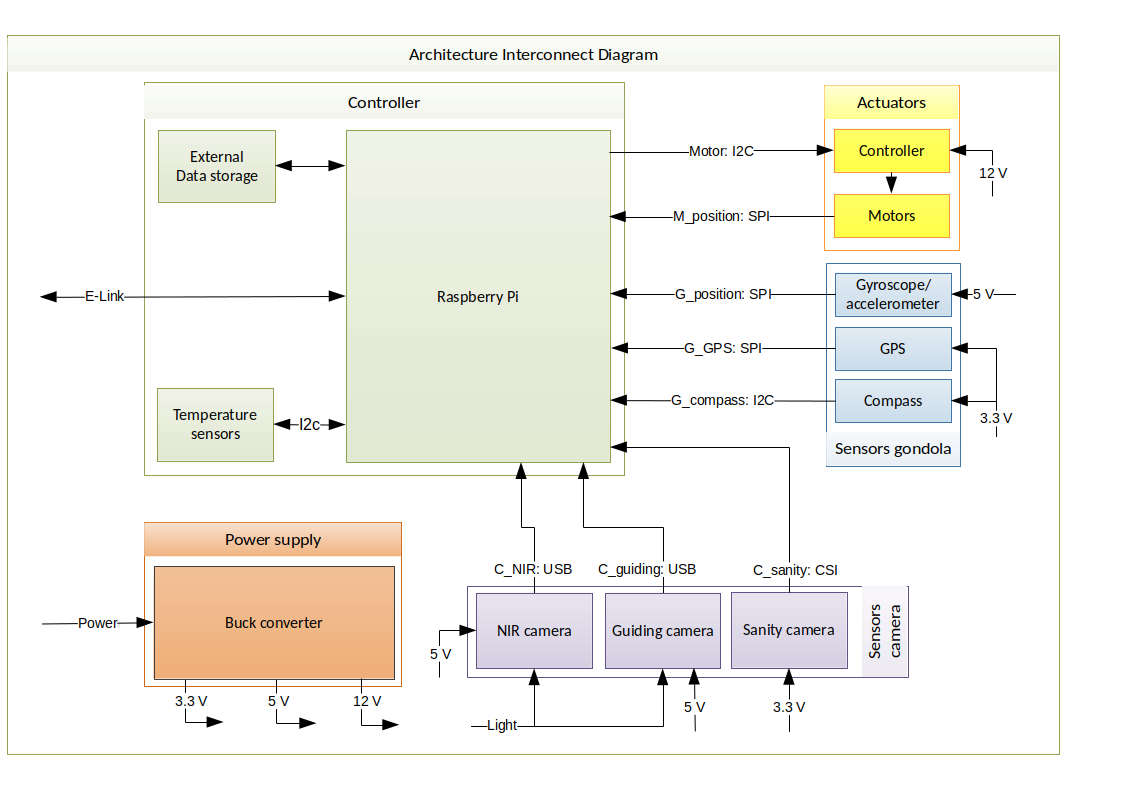
\includegraphics[width=.85\textwidth]{4-experiment-design/img/electrical/ArchitectureInterconnect.png}
	\caption{Electrical architecture interconnect diagram.}
	\label{fig:elec-AID}
\end{figure}

\subsubsection{Motor-controller \& Motor}
When putting a PWM signal on a DC-motor, the position of the DC-motor can be controlled as well as the speed between two positions. The inputs of the motors will always be inverted to each other. This is how a servo motor works as well and will be implemented to position the telescope.\\

The amount of steps per duty cycle of the pwm signal is 12 bits with the PCA9685 chip. This means $2^{12}$ steps between full on and full off. This will result that the motors can turn very very slowly.\\

Then the signal will be amplified in current with a L298 motor driver (H-bridge). This signal will be delivered to a DC-motor which is geared with 1:312. There will be an encoder before and after the gearbox. As most high encoders aren't able to measure below 5 arcseconds. Measuring before the gearbox helps to take smaller steps.\\

The chosen encoder is an AMT23. This encoder has $2^{14}$ positions. When measuring before the gearbox, each step corresponds with 0.25 arcseconds. But because the motor can bounce between two bits the effective resolution is 0.5 arcseconds. The second encoder behind the gearbox has at least 312 steps per rotation, this way the position of the telescope can be measured exactly. Since the encoders are absolute encoders and measure independently of the OBC, a watchdog reboot will not affect these measurements.


\subsubsection{Gyroscopes}
We are currently talking to Honeywell to borrow the GG1320AN Digital Ring Laser Gyroscopes. This will improve the design by a lot and the previous designed gyroscopes below will no longer be used.\\

The current defined gyroscope is the ADXRS624. The main parameter is the noise from the gyroscope is the noise, which is 0.04\,$^\circ/ \sqrt{f_s}$, with $f_s$ being the sampling frequency. This means that a sampling frequency of 80 kHz, this system should be able to stay within the 0.5 arcseconds accuracy. For redundancy it might be necessary to have a dedicated microcontroller for the signal processing. This chip can only measure differences from its 0$^\circ$ position up to 75$^\circ$, but this should be sufficient enough as we can reset the 0$^\circ$ position between images.\\

This chip is analog and must be read out by an ADC that is able to read out the signal with a high enough accuracy on that specific sampling frequency. For this the AD7175 ADC is chosen. With a sampling frequency of 250,000\,Hz the effective resolution is 20.1 bits or 8.7\,$\mu$V. The gyroscope gives a change is voltage of 18\,$\mu$V per arcsecond. Thus everything below 9\,$\mu$V should be sufficient to measure with 0.5 arcseconds accuracy.


%\subsubsection{Star tracker}
%TODO : ADD THIS DECRIPTION
%\colorbox{yellow}{\parbox{\textwidth}{}}

\subsubsection{Schematic}
See Appendix c.

\subsubsection{PCB Layout}
There will be three PCB:s, which are listed below:

\begin{itemize}
	\item 	Power system, motor control \& temperature actuator control.
	\item	Accelerometer, GPS, compass, temperature sensors
	\item 	Gyroscopes
\end{itemize}



The two PCB's for the power system, motor control, temperature, accelerometer, GPS and compass, will be located in the electronics box. They will be placed on top of each other. Also the controller will be mounted in this electronics box. %, see figure \ref{fig:electronic-box}

%\begin{figure}[H]
%	\centering
%	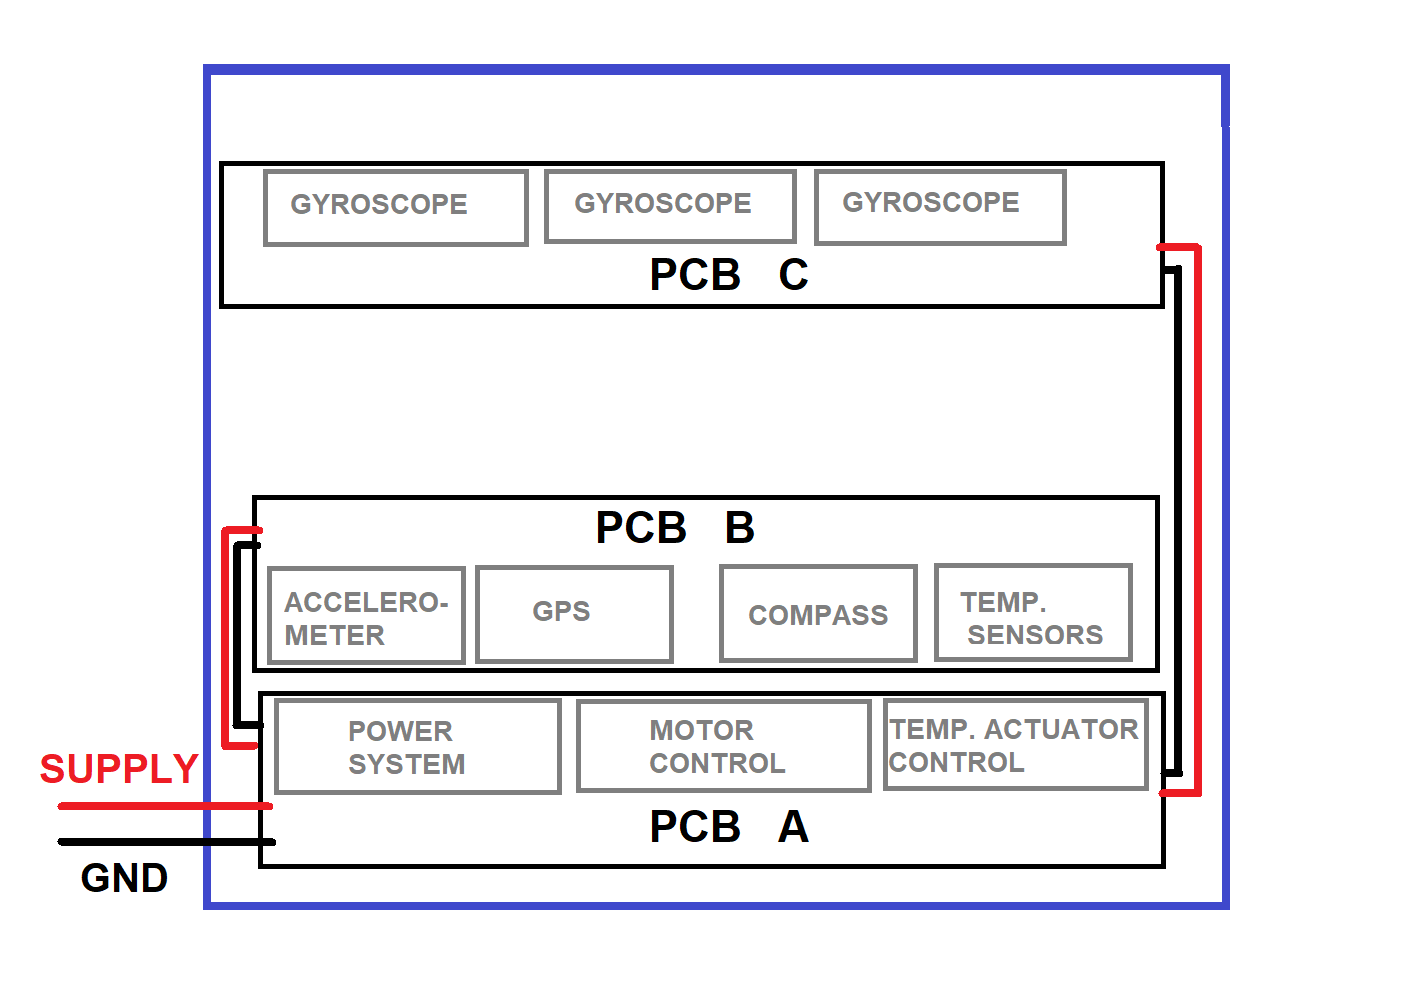
\includegraphics[width=\textwidth]{4-experiment-design/img/electrical/ElectricalBox.png}
%	\caption{An architecture diagram of the electronics.}
%	\label{fig:electronic-box}
%\end{figure}


The third PCB will be placed in its own second electronics box because it includes the gyroscopes. Thus the PCB should not be too close to the other PCBs or the DC motors due to disturbances, such as for example magnetic field changes. The schematics of all the PCBs can be found in appendix C.
\raggedbottom

\pagebreak
\subsection{Thermal Design} 
\label{Thermal_section}















\subsubsection{Thermal requirements}

\paragraph{Operating temperatures}

The most obvious temperature requirement was in meeting the operating temperature for the various components, tabulated below.\\ 

% highy recommend https://www.tablesgenerator.com/

\begin{center}
\begin{table}[H]
\centering
\footnotesize
\begin{tabular}{ | l | c | c |}
    \hline
    \textbf{Component} & \textbf{Component no.} & \textbf{Operating temp [\textsuperscript{o}C]} \\ 
    \hline
    Accelerometer & KXTJ3-1057CT-ND & -40 – 85 \\ 
    \hline
    ADC AD7175 & 835-3826 & -40 – 105 \\ 
    \hline
    ADC AD7997 & 697-7170 & -40 – 85 \\ 
    \hline
    Antenna & 704-3449 & -40 – 85 \\ 
    \hline
    Buck converter 3.3V & 296-40220-1-ND & -40 – 125 \\ 
    \hline
    Buck converter 5V 4A & 785-1689-1-ND & -40 – 85 \\ 
    \hline
    Buck converter 12V 1.25A & LM2695MH/NOPB-ND & -40 – 125 \\ 
    \hline
    Camera Raspberry Pi V2 & 301-34-462 & -20 – 60 \\ 
    \hline
    Camera  ZWO ASI183MM & IMX183CLK-J & -5 – 45 \\ 
    \hline
    Capacitor 1 uF & 301-19-869 & -55 – 125 \\ 
    \hline
    Capacitor 1.4 pF & 300-47-684 & -55 – 125\\ 
    \hline
    Capacitor 22 nF & 300-65-997 & -55 – 125 \\ 
    \hline
    Capacitor 44 pF (47 pF) & 300-67-381 & -55 – 125 \\ 
    \hline
    Capacitor 850 pF & 165-81-144 & -55 – 125 \\ 
    \hline
    Capacitor 0.47 uF (420 nF) & 300-87-046 & -55 – 125 \\ 
    \hline
    Capacitor 0.1 uF & 165-73-687 & -55 – 125 \\ 
    \hline
    Capacitor 1 uF & 165-61-179 & -55 – 125 \\ 
    \hline
    Capacitor 2.2 uF & 165-71-988 & -55 – 125 \\ 
    \hline
    Capacitor 3 uF (3.3 uF) & 165-71-996 & -55 – 125 \\ 
    \hline
    Capacitor 4 uF (4.7 uF) & 300-31-816 & -55 – 125 \\ 
    \hline
    Capacitor 32 uF (33 uF) & 915-5461 & -55 – 125 \\ 
    \hline
    Capacitor 10 uF & 301-12-804 & -55 – 125 \\ 
    \hline
    Capacitor 4.7 uF & 300-31-677 & -55 – 85 \\ 
    \hline
    Capacitor 0.1 uF & 300-67-806 & -55 – 125 \\ 
    \hline
    Compass & MLX90393SLW-ABA-011 & -20 – 85 \\ 
    \hline
    Crystal 16 MHz, 9 pF, 10ppm & 301-09-485 & -40 – 85 \\
    \hline
    Encoder & 102-4485-ND & -40 – 105 \\
    \hline
    Ferrite Bead 600Ohm @ 100MHz & 724-1545 & -55 – 125 \\
    \hline
    GPS & NEO-M8N & -40 – 85\\
    \hline
    Gyroscope & EVAL-ADXRS624Z-ND & -55 – 125 \\
    \hline
    Inductor 68 uH & 300-37-257 & -40 – 105 \\
    \hline
    Inductor 24 uH (22 uH) & 158-00-313 & -20 – 105 \\
    \hline
    Inductor 22 uH & 110-63-696 & -40 – 155\\
    \hline
    Igarashi DC Gearmotor & 1711491-62 & 0 – 60 \\  
    \hline
    Microcontroller & 636-384 & -25 – 130 \\
    \hline
    Peltier cooler & PE-031-10-15-S & 0 – 74 \\
    \hline
    PWM expander & 727-5649 & -40 – 85 \\
    \hline
    Raspberry Pi Zero (no WiFi) & 1910-1104-ND & 0 – 70 \\
    \hline
    Raspberry Pi 3B+ & 137-3331 & 0 – 50 \\
    \hline
    Schottky diode & 170-09-098 & -50 – 150 \\
    \hline
    Temp sensor & 301-29-188 & -55 – 150 \\
    \hline
    Transistor NPN 15nA leak & 300-32-503 & -65 – 150 \\
    \hline
    Transistor PNP & 300-41-424 & -50 – 150 \\
    \hline
    U-regulator & 173-88-854 & -50 – 125\\
    \hline
\end{tabular}
\caption{The operating temperature for each component of the experiment.}
\end{table}
\label{tab: temp ranges}
\end{center}

As the ambient conditions were likely to be very cold, many of the components would need to be heated so that the electronics would be able to operate.\\

The motors would need to be maintained at between 0\textsuperscript{o}C and 60\textsuperscript{o}C. If the ambient conditions were assumed to be -70\,\textsuperscript{o}C, then the temperature of these motors would need to be raised by more than 80\,\textsuperscript{o}C, assuming a tolerance of 10\,\textsuperscript{o}C.\\

The main camera (ZWO ASI183MM) would need to be maintained at between -5\textsuperscript{o}C and 45\textsuperscript{o}C. The temperature of this component would need to increase by more than 75\,\textsuperscript{o}C. Likewise for the guiding camera. For the main camera to reduce noise there was value in keeping the optics cool while the electronics were warmed to the operating temperature. This was taken into account in the thermal design.\\

The sanity camera (Raspberry Pi Camera v2.1) would need to be maintained at between -20\textsuperscript{o}C and 60\textsuperscript{o}C. The temperature of this component would need to increase by more than 60\,\textsuperscript{o}C.\\

For the electronics box, the temperature would need to be between 0\textsuperscript{o}C and 50\textsuperscript{o}C, for the Raspberry Pi, the most temperature sensitive component. A temperature increase of more than 80\textsuperscript{o}C was required\textsuperscript{o}C.\\

\paragraph{SNR}

In order to ensure minimal measurement error in acquiring images, the effect of temperature on the optics had to be considered, and the temperature had to be controlled if needed to ensure that the error is within an acceptable range.\\

Dark current is small residual currents that are present in the camera, generated irrespective of whether there is incident illumination. This dark current becomes present in the data in the form of random noise that is not trivial to subtract. By decreasing the operating temperature of the camera optics, the magnitude of dark current can be minimised and the signal to noise ratio increased. This relationship between signal to noise ratio and dark current is as follows\\

\begin{center}
 $SNR =  \frac{I\times QE\times t}{\sqrt{I\times QE\times t+Nd\times t+Nr^2}}$\\
\end{center}

$I$ = Photon flux (photons/pixel/s)\\
$QE$ = Quantum efficiency\\
$t$ = Integration time (s)\\
$Nd$ = Dark current (electrons/pixel/s)\\
$Nr$ = Read noise (electrons)\\

The ASI183 camera is specified as having a read noise of 1.6e @30db gain and a QE peak of 84\%. The camera also has the following relationship between dark current and sensor temperature. Calculations will be considered for an exposure time of 300s, which was the longer intended exposure time for higher quality imaging.  \\


	\begin{figure}[H]
    \centering
    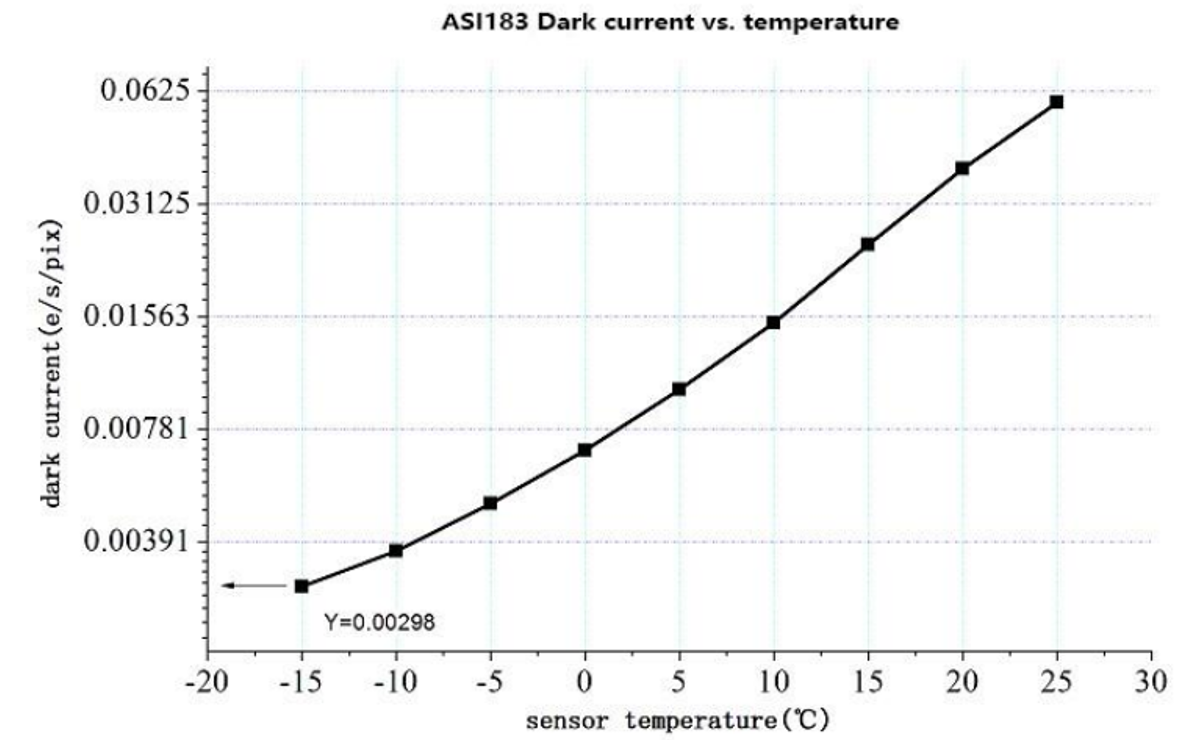
\includegraphics[scale=0.8]{4-experiment-design/img/mechanical/darkcurrent.png}
    	\caption{Dark current through the camera at various temperatures. Source: ZWO}
	\label{fig:darkcurrent}
	\end{figure}

As an example, the SNR as affected by dark current at -10\,\textsuperscript{o}C versus 10\,\textsuperscript{o}C is\\

 SNR(-10\,\textsuperscript{o}C) =  $\frac{(\SI{6.16}{photons \per pixel \per sec})\times (0.84)\times (\SI{300}{s})}{\sqrt{(\SI{6.16}{photons \per pixel \per s})\times (0.84)\times (300s)+(\SI{0.00391}{e \per pixel \per s})\times (\SI{300}{s})+(\SI{1.6}{e})^2}}$ \\

 SNR(-10\,\textsuperscript{o}C) = 39.35\\

 SNR(10\,\textsuperscript{o}C) =  $\frac{(\SI{6.16}{photons \per pixel \per sec})\times (0.84)\times (300s)}{\sqrt{(\SI{6.16}{photons \per pixel \per s})\times (0.84)\times (\SI{300}{s})+(\SI{0.01563}{e \per pixel \per s})\times (\SI{300}{s})+(\SI{1.6}{e})^2}}$ \\

 SNR(10\,\textsuperscript{o}C) = 39.31\\


\paragraph{Optothermal stability}
Another important effect would be the how thermal stresses and subsequent deflections could affect the optics of the camera, in particular the index of refraction, and hence the quality of the collected data. Variation of solar flux over the time of flight and from the heat signatures of the BEXUS module would need to be considered. A thermoelastic analysis should be conducted in finite element analysis software to evaluate the effects of the thermal environment, and the implication of those results on the validity of the data should be investigated. \

\paragraph{Condensation}
Condensation could occur if air heated by the camera heating elements was able to condensate on the cold surfaces of the optics. This would deteriorate the quality of the detections and must had to be mitigated.  \

	\begin{figure}[H]
    \centering
    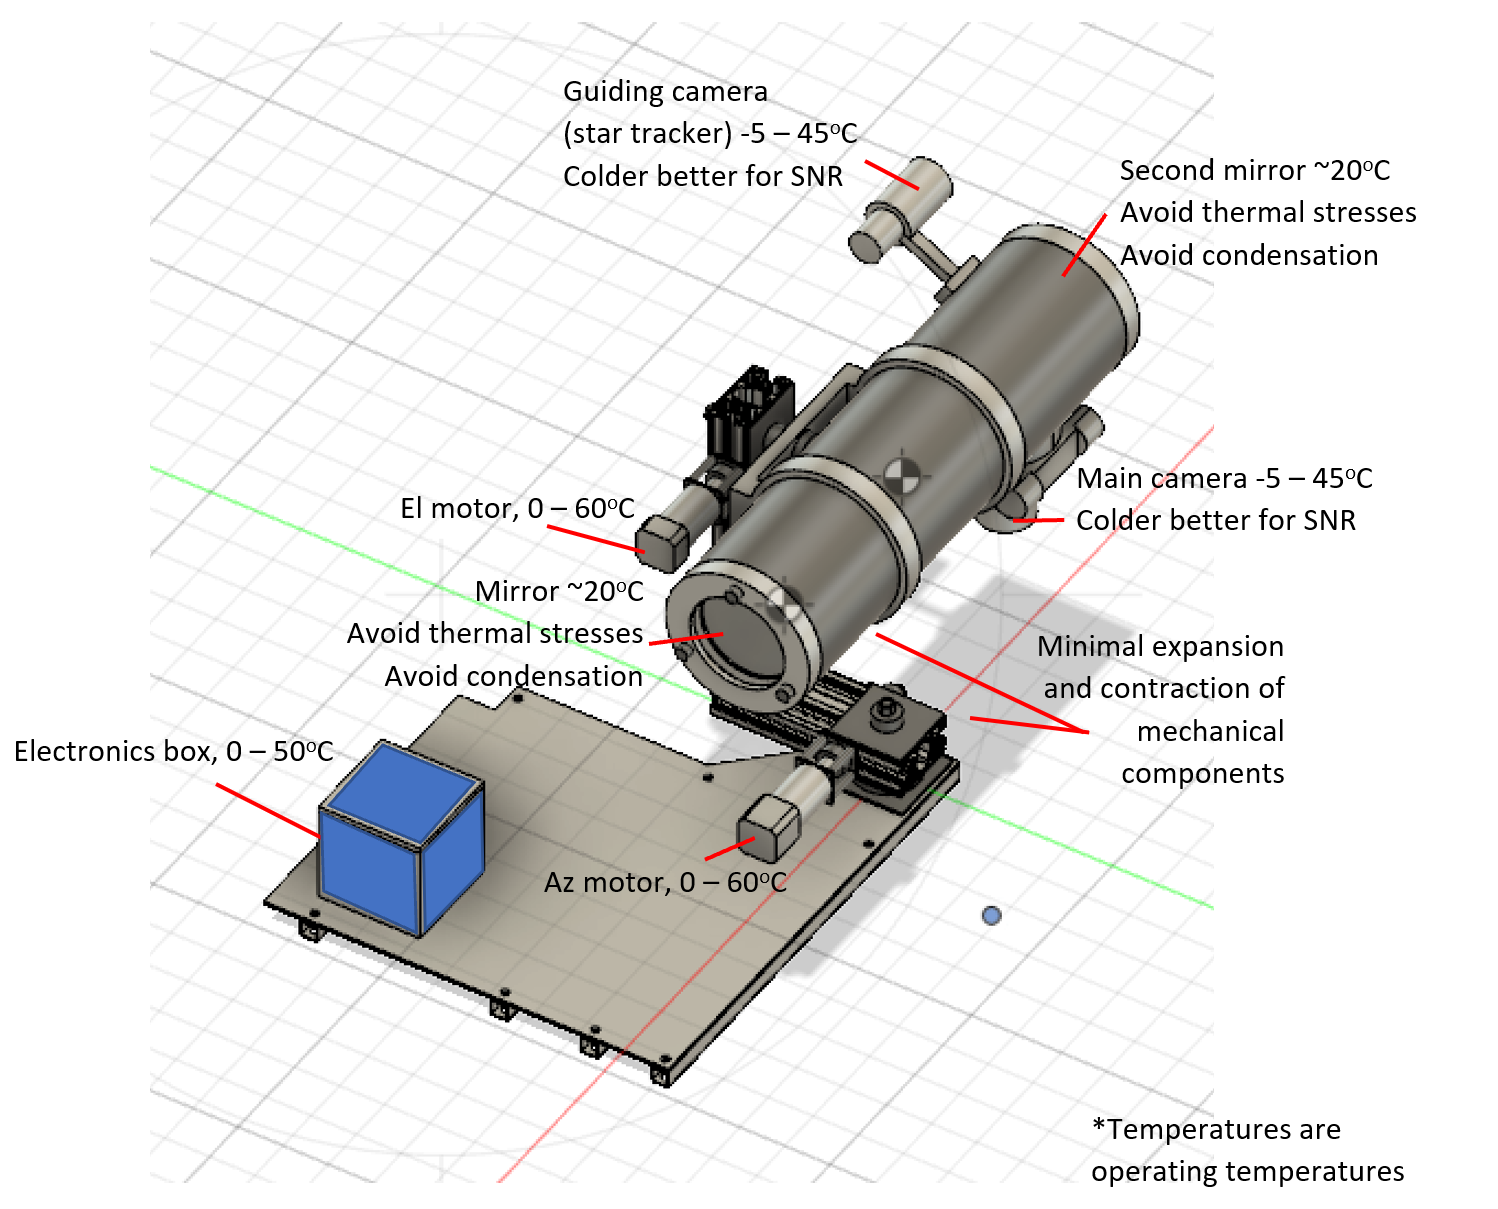
\includegraphics[scale=0.8]{4-experiment-design/img/mechanical/thermalrequirements.PNG}
    	\caption{Summary of the thermal requirements for the system.}
	\label{fig:thermalrequirements}
	\end{figure}





\subsubsection{Thermal environment}
\paragraph{Atmosphere ambient conditions}
IRISC would ascend to and float in the stratosphere at an altitude of between 25 and 30\,km, after which it would experience altitude fluctuations of no more than 200\,m. This would be the phase of flight during which the infrared camera would be operational and hence thermal control most necessary in ensuring sound optical performance. This part of the atmosphere is also characterised by relatively low temperatures. Based on the flights of a number of previous BEXUS missions seen in the graph of the atmosphere, it could be assumed that the atmospheric temperature during float would range between -70\,\textsuperscript{o}C and -50\,\textsuperscript{o}C. \\

	\begin{figure}[H]
    \centering
    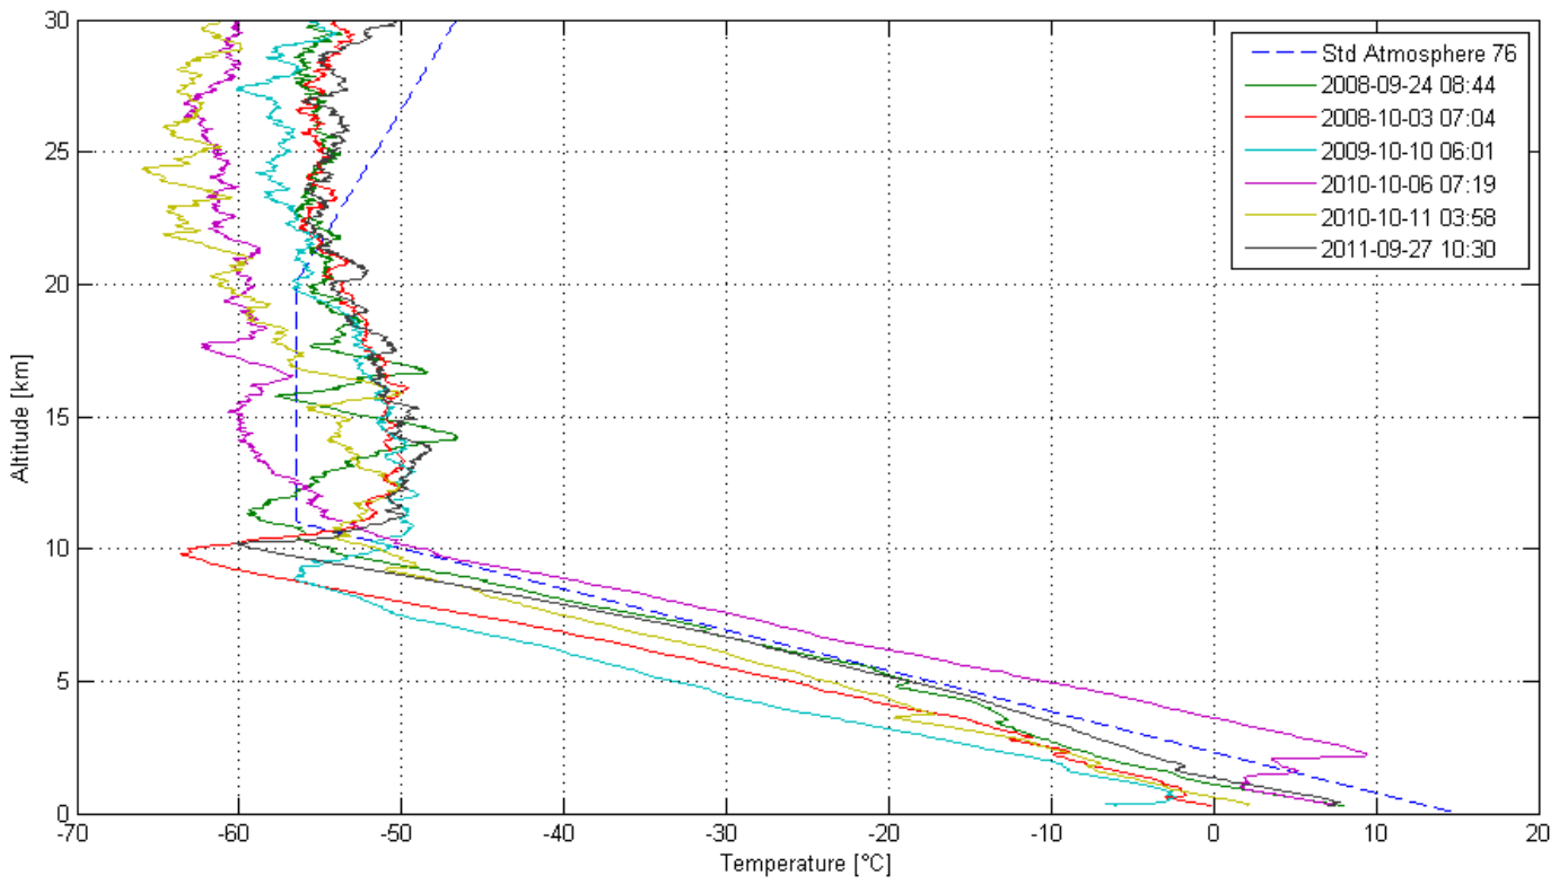
\includegraphics[scale=0.58]{4-experiment-design/img/mechanical/atmosphere.PNG}
	\caption{Temperature profile of the atmosphere. Source: REXUS/BEXUS}
	\label{fig:atmosphere}
	\end{figure}

% highy recommend https://www.tablesgenerator.com/

\begin{center}
\begin{table}
\centering
  \begin{tabular}{ | l | c | r | }
    \hline
    \textbf{Flight phase} & \textbf{Expected temperature} & \textbf{Duration} \\ \hline
    Preparation  & 15 – 25\,\textsuperscript{o}C & 4 hours \\ \hline
    Launch pad wait & -15 – 0\,\textsuperscript{o}C & 3 hours \\ \hline
    Ascent phase  & -80 – 0\,\textsuperscript{o}C & 1.5 hours \\ \hline
    Float phase (25-30km) & -70 – -50\,\textsuperscript{o}C & 1 – 5 hours \\ \hline
    Descent phase  & -80 – 0\,\textsuperscript{o}C & ~ 30 minutes \\ \hline
    Post-flight phase & -15 – 0\,\textsuperscript{o}C & 1 – 2 days \\ \hline
  \end{tabular}
\caption{\hl{The temperature expected for each phase of the BEXUS campaign.}}
\end{table}
\label{tab: flight phases}
\end{center}

\paragraph{Solar flux}

The extent of solar irradiance was characterised by several factors, including the sun’s height above the horizon, typically low for the polar latitudes that the balloon would be flying at, and the height in the atmosphere and atmospheric conditions, which would cause absorption and scattering of light. \\
The total solar irradiance, neglecting atmospheric effects, at the Esrange latitude of 68\textsuperscript{o} and assuming a launch date of the 15th of October is demonstrated in the following graph of direct solar radiation, with a peak of ~500\,W/m\textsuperscript{2} at noon.\\

	\begin{figure}[H]
    \centering
    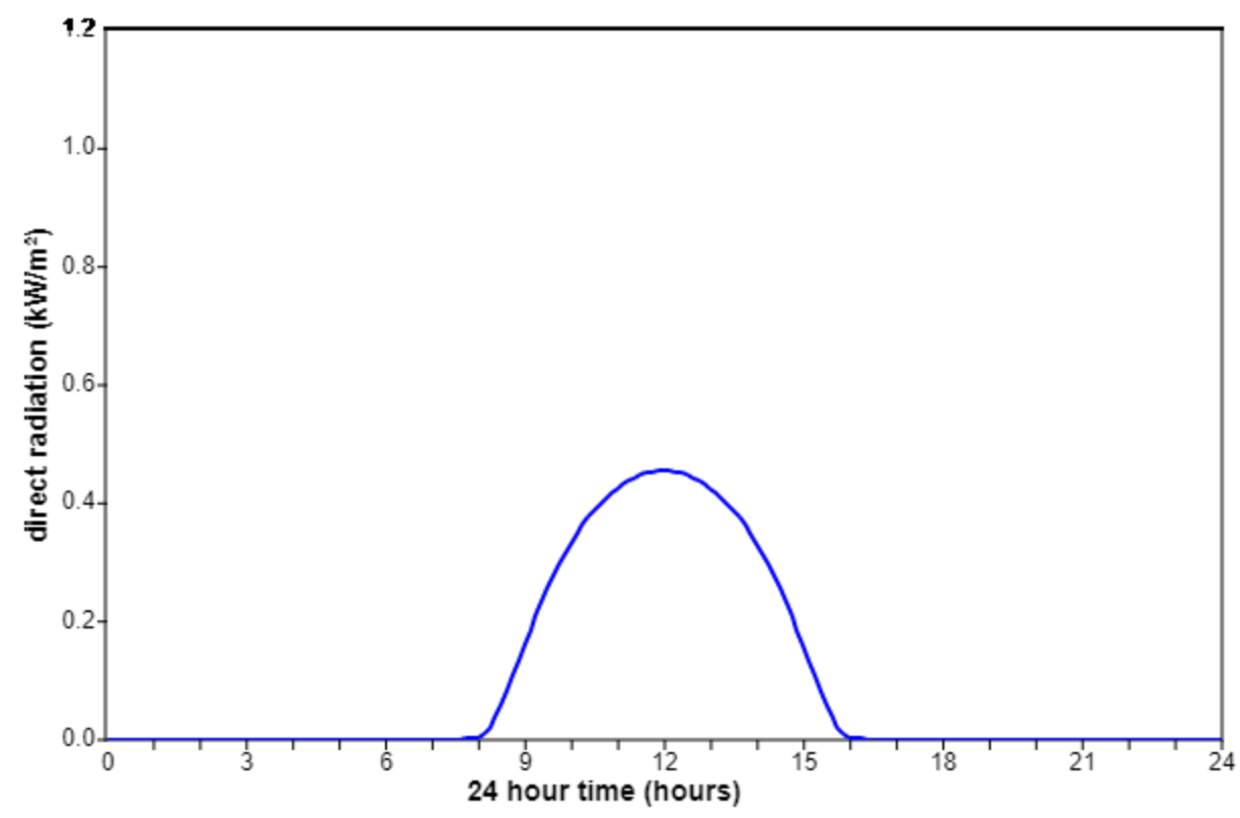
\includegraphics[scale=0.6]{4-experiment-design/img/mechanical/directradiation.png}
	\caption{Estimate of direct solar radiation at the top of the atmosphere. Source: PVeducation.org}
	\label{fig:directradiation}
	\end{figure}

The degree of attenuation of solar radiation through the atmosphere can be described using the Beer–Lambert law, which relates the transmittance of radiation to optical depth. For an atmosphere with properties that change exponentially with respect to altitude, the optical depth can be estimated to also change exponentially with respect to altitude. \\

\paragraph{Internal heat generation}
Another factor affecting the thermal environment comes from the generation of heat by the electronic components in the electronics box, from each camera, and from each motor. This heat is generated from losses of the supplied power through electrical and mechanical processes. An estimate of the power drawn by each component was conducted.

% highy recommend https://www.tablesgenerator.com/

\begin{center}
\begin{table}
\centering
    \begin{tabular}{ | l | c | }
    \hline
    \textbf{Component} & \textbf{Power drawn [W]}\\ 
    \hline
    Raspberry Pi 3B+  & 10\\
    \hline
    Gyroscope & 0.02\\ 
    \hline
    GPS  & 0.03\\ 
    \hline
    PWM controller & 0.05\\ 
    \hline 
    Encoders  & 0.04 \\ 
    \hline
    Accelerometer  & negligible \\ 
    \hline
    Temperature sensors  & negligible \\ 
    \hline
    Buck converter 3.3V  & 0.183 \\ 
    \hline
    Buck converter 5V  & 1.67 \\ 
    \hline
    Buck converter 12V  & 3.75 \\ 
    \hline
    \textbf{Total in electronics box}  & \textbf{15.78} \\ 
    \hline
    \textbf{DC motor 1}  & \textbf{1.4} \\
    \hline
    \textbf{DC motor 2}  & \textbf{1.4} \\ 
    \hline
    \textbf{DC motor 3}  & \textbf{1.4} \\
    \hline
    \textbf{Guiding camera}  & \textbf{1.5} \\
    \hline
    \textbf{Sanity camera}  & \textbf{0.825} \\ 
    \hline
    \textbf{Main camera}  & \textbf{1.5}\\ 
    \hline
  \end{tabular}
\caption{\hl{The power drawn by each component of the experiment.}}
\end{table}
\label{tab: thermal power}
\end{center}

The DC gear motors are rated as having a maximum efficiency of 35\%. 
For electronics that consume all supplied power, such as the cameras and Raspberry Pi, all power will be converted to heat.
For other electronic components, it will be assumed that they are 90\% efficient. By multiplying the supplied power by the efficiencies, the heat generation can be determined.

% highy recommend https://www.tablesgenerator.com/

\begin{center}
\begin{table}
\centering
 \begin{tabular}{ | l | c | }
    \hline
    \textbf{Component} & \textbf{Heat generation [W]}\\ 
    \hline
    \textbf{Electronics}  & \textbf{\hl{10.58}} \\ 
    \hline
    \textbf{DC motor 1}  & \textbf{0.91} \\
    \hline
    \textbf{DC motor 2}  & \textbf{0.91} \\ 
    \hline
    \textbf{DC motor 3}  & \textbf{0.91} \\
    \hline
    \textbf{Guiding camera}  & \textbf{\hl{1.5}} \\
    \hline
    \textbf{Sanity camera}  & \textbf{\hl{0.825}} \\ 
    \hline
    \textbf{Main camera}  & \textbf{\hl{1.5}}\\ 
    \hline
  \end{tabular}
\caption{\hl{The heat generated by each component of the experiment.}}
\end{table}
\label{tab: heat generated}
\end{center}

It is of note that in historical BEXUS projects utilising the Raspberry Pi in an insulated environment, surface temperatures of 50\textsuperscript{o}C have been recorded. 





















\subsubsection{Thermal analysis}

\paragraph{Insulation for electronics box}

In the electronics box, a substantial amount of heat is generated by the electrical components and in particular the Raspberry Pi. This heat will convect and radiate out to the colder surroundings. By quantifying the heat generation and comparing it to the heat losses, the temperature inside the box can be determined. The heat loss can be controlled by adding an insulating layer around the box, which will resist the conduction of energy to the surface of the box. In this case, extruded polystyrene will be used as the material, due to its low conductivity and because it is less resistant to thermal expansion. \\

An analysis of the heat loss for the electronics box maintained at 20\textsuperscript{o}C was conducted. \\

	\begin{figure}[H]
    \centering
    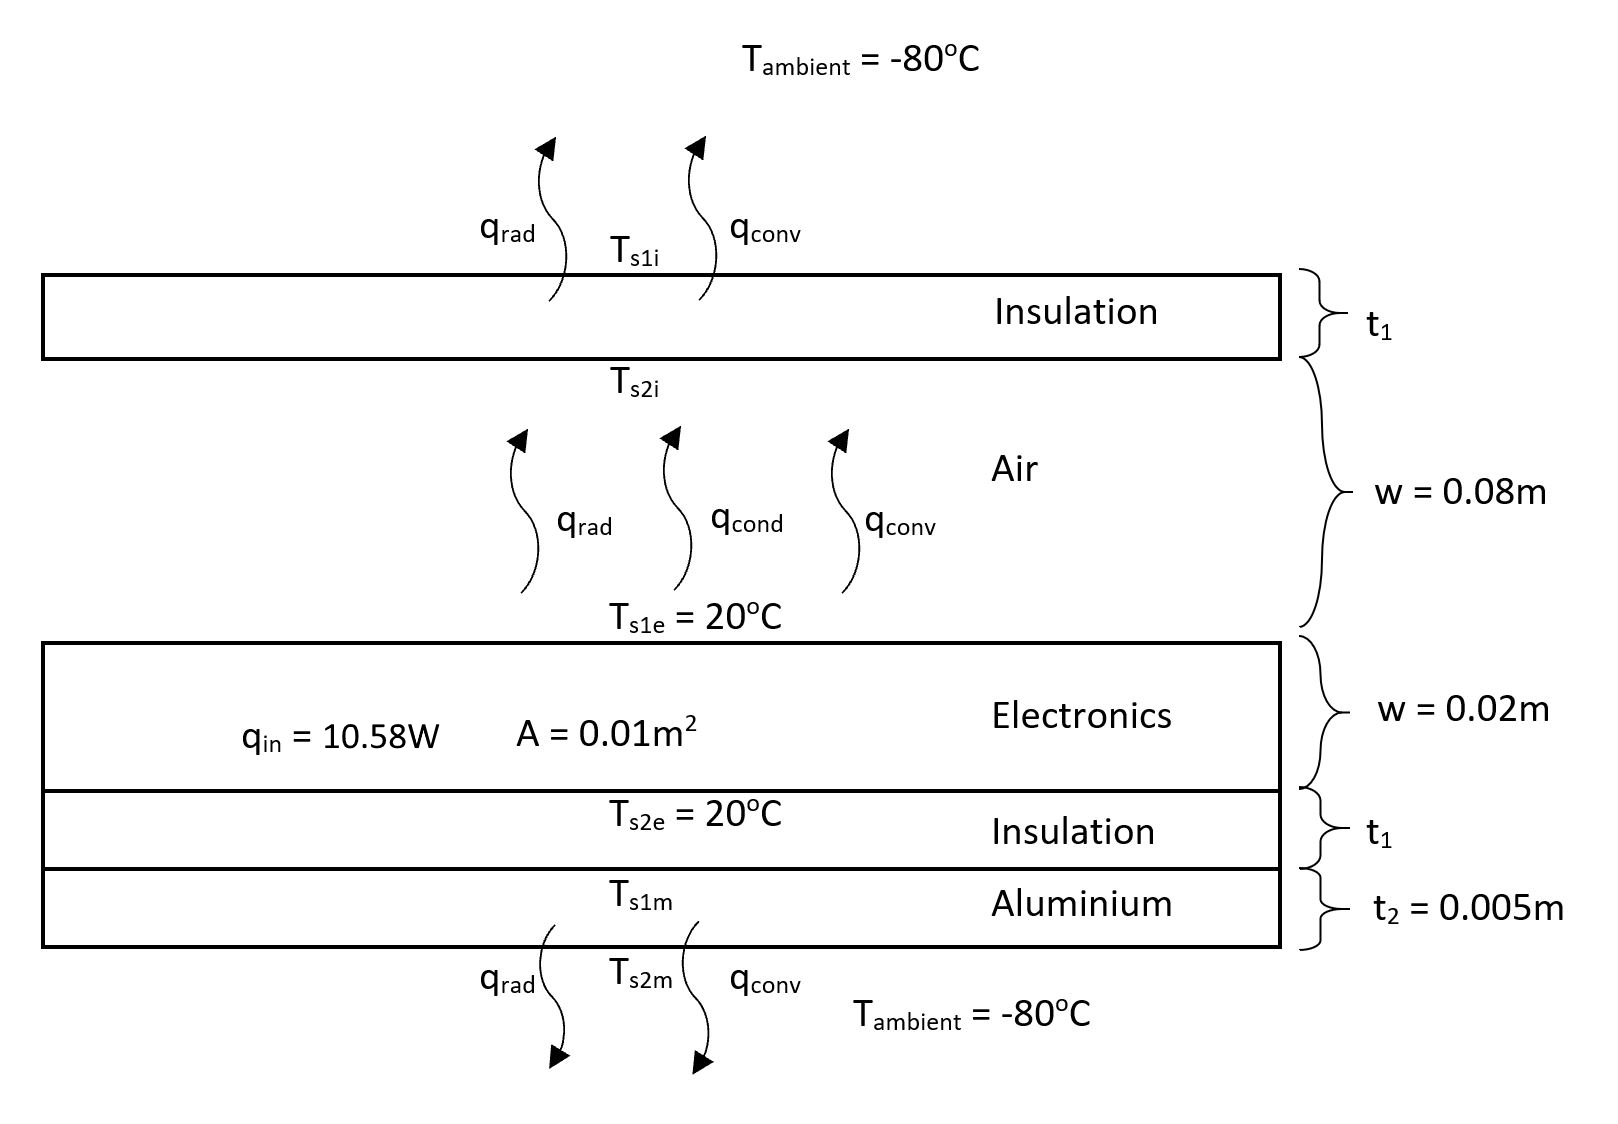
\includegraphics[scale=0.6]{4-experiment-design/img/mechanical/thermaldiagram.JPG}
	\caption{Heat transfer model of the electronics box.}
	\label{fig:thermaldiagram}
	\end{figure}

The material properties are as follows: \\

Thermal conductivity of insulation: $ k_{i} = 0.034 \frac{W}{m K} $ \\
Thermal conductivity of aluminium: $ k_{m} = 205 \frac{W}{m K} $ \\
Thermal conductivity of air at 1 kPa, -80\textsuperscript{o}C: $ k_{a} = 15\times10^{-3} \frac{W}{m K} $ \\ 
Convective heat transfer coefficient of air: $ h_{a,c} = 3.12 \frac{W}{m^{2} K} $ \\ 
Radiative heat transfer coefficient of air: $ h_{a,r} = 6.59 \frac{W}{m^{2} K} $ \\ 

For 1D steady state conduction through the composite wall comprised of insulation and aluminium: \\

	\begin{figure}[H]
    \centering
    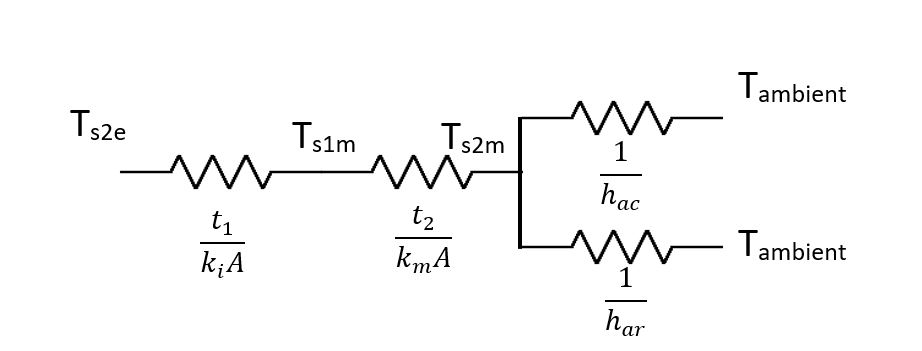
\includegraphics[scale=0.6]{4-experiment-design/img/mechanical/thermalresistance1.JPG}
	\caption{Thermal resistance for bottom of box.}
	\label{fig:thermalresistance1}
	\end{figure}

\begin{center}
 $q_{cond1} = \frac{T_{s2,e}-T_{ambient}}{R_{tot}} $\\
 
 \ 
 
 $R_{tot} = \frac{t_{1}}{k_{i}A} + \frac{t_{2}}{k_{m}A} + \frac{1}{h_{a,e}+h_{a,m}} $\\
 
 \
 \ 
 
 $q_{cond1} = \frac{293.15 - 193.15}{\frac{t_{1}}{(0.034)(0.01)} + \frac{0.005}{(205)(0.01)} + \frac{1}{3.12+6.59}} $\\
 
 \  
 \ 
 
 $q_{cond1} = \frac{100}{2940t_{1}+0.105} $\\
 
\end{center}
 

For 1D steady state conduction through the upper insulating layer: \\

	\begin{figure}[H]
    \centering
    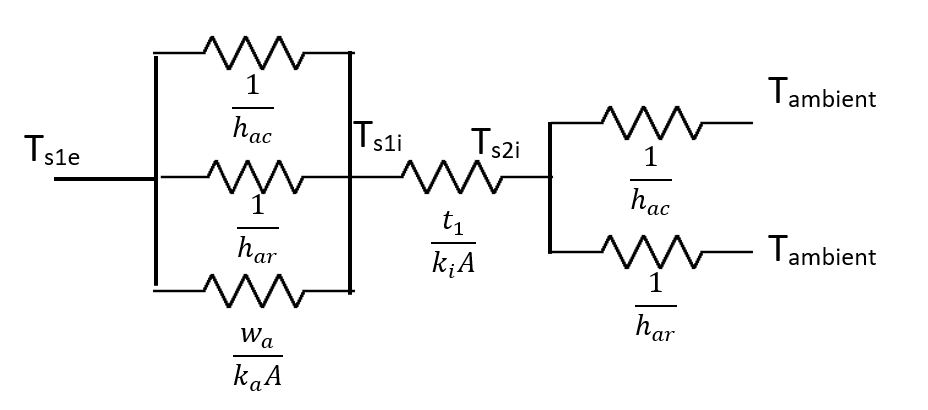
\includegraphics[scale=0.6]{4-experiment-design/img/mechanical/thermalresistance2.JPG}
	\caption{Thermal resistance for top of box.}
	\label{fig:thermalresistance2}
	\end{figure} 

\begin{center}
 $q_{cond2} = \frac{T_{s1,e}-T_{ambient}}{R_{tot}} $\\
 
 \ 
 
 $R_{tot} = \frac{1}{h_{a,e}+h_{a,m}+\frac{k_{a}A}{w_{a}}} + \frac{t_{1}}{k_{i}A} + \frac{1}{h_{a,e}+h_{a,m}}  $\\
 
 \
 \ 
 
 $q_{cond2} = \frac{293.15 - 193.15}{\frac{1}{3.12+6.59+\frac{(15\times10^{-3})(0.01)}{0.08}} + \frac{t_{1}}{(0.034)(0.01)} + \frac{1}{3.12+6.59}} $\\
 
 \  
 \ 
 
 $q_{cond2} = \frac{100}{2940t_{1}+0.206} $\\
 
\end{center}

By summing the heat lost on both sides and equating that to the heat generated, we can find the thickness of insulating material to maintain the constant temperature. \\

\begin{center}
 $q_{loss} = \frac{100}{2940t_{1}+0.105} + \frac{100}{2940t_{1}+0.206} =$ 
10.58 W
$= q_{gain} $\\
\end{center}

Solving this equation yields a thickness of 0.64\,cm. It is important to note that this analysis relies on several assumptions, such as one dimensional steady state heat transfer, and that the convection mechanism on the top and bottom of the electronics box is the same. It also does not take into account heat flux from solar radiation. In reality, there will be a conductive path through the insulating material from the bottom to the top of the box, and heat will not have to pass through the very low density air in the box. This will be taken into account in a FEA analysis of the thermal properties, using the ANSYS package. \\

To verify the results on the analytical study of the electronics box thermal scenario, a model was created and analysed using the FEA tool built into Autodesk Fusion 360. A simple model was considered using the same dimensioned box attached to a $350 \,mm \times 450\,mm \times 6\,mm$ sheet of aluminium metal that the box can gradually conduct heat into through the insulation. \\

A $100\,mm \times 100\,mm \times 20\,mm$ box of epoxy resin is placed in the inside of the box, so that it is in contact with the inside walls. This box is a crude representation of the PCB and is modelled to have the 10.58 W of heat generated uniformly through the material, representing the heat generated by the Raspberry Pi.\\

In addition to the 10.58 W of heat from the electronics box, 500 $\frac{W}{m^{2}}$ of heat was modelled as being incident on the top surface of the aluminium base and the electronics box. The system loses heat through radiation and convection of the largest surfaces to a -80\textsuperscript{o}C environment.

The materials and corresponding properties are as follows:

% highy recommend https://www.tablesgenerator.com/

\begin{center}
\begin{table}[ht]
\centering
\resizebox{\textwidth}{!}{\begin{tabular}{ | l | c | c | c | c | c | }
    \hline
    \textbf{Material} & \textbf{Components} & \textbf{Density $ \frac{kg}{m^3} $ } & \textbf{Conductivity $ \frac{W}{m ^oC} $} &\textbf{Specific heat $ \frac{J}{^oC kg} $} & \textbf{Emissivity / absorptivity  ratio (-)} \\ \hline
    Epoxy resin  & PCB & 1140 & 0.468 & 1000 & -\\ \hline
    Aluminium & Base & 2700 & 230 & 897 & 0.46\\ \hline
    Polystyrene (extruded)  & Box, Lid & 35 & 0.027 & 1470 & 0.9\\ \hline
  \end{tabular}}
\caption{\hl{Thermal properties of the materials used in the FEA simulation, with polystyrene radiating more readily and aluminium conducting more readily.}}
\end{table}
\label{tab: thermal materials}
\end{center}

The convection constant of air at 1000 Pa, 3.12 $\frac{W}{m^2 K} $ was selected as for the previous analysis.

A static thermal analysis was therefore conducted under these conditions for an insulation thickness of 1 mm, 3 mm, and 6 mm.

	\begin{figure}[H]
    \centering	
	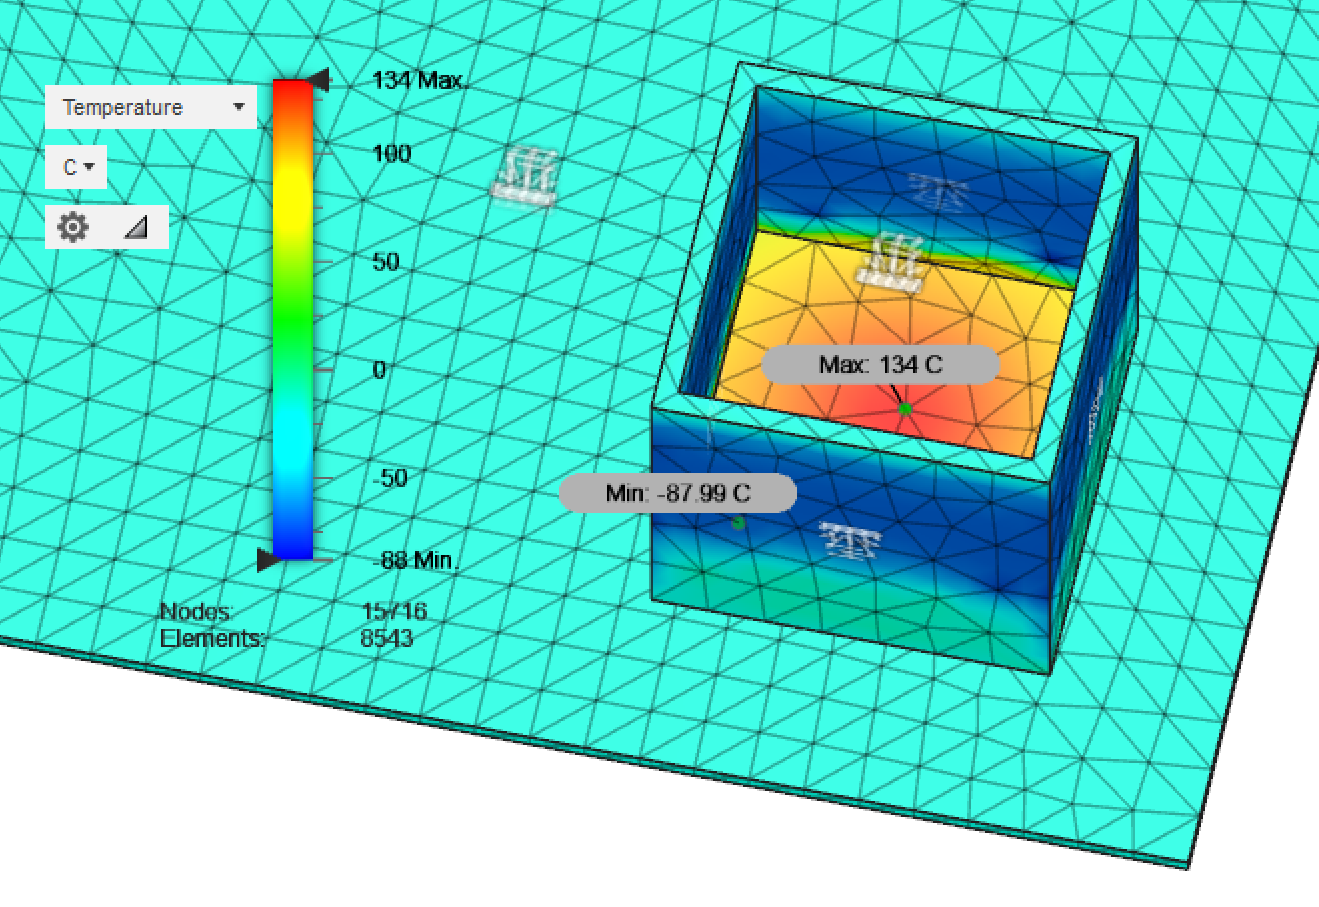
\includegraphics[scale=0.58]{4-experiment-design/img/mechanical/6mmthickheat.PNG}
	\caption{Thermal simulation of electronics box with 6mm insulation, exposed to solar heating.}
	\label{fig:6mmthickheat}
    	\end{figure}

	\begin{figure}[H]
    \centering    	
    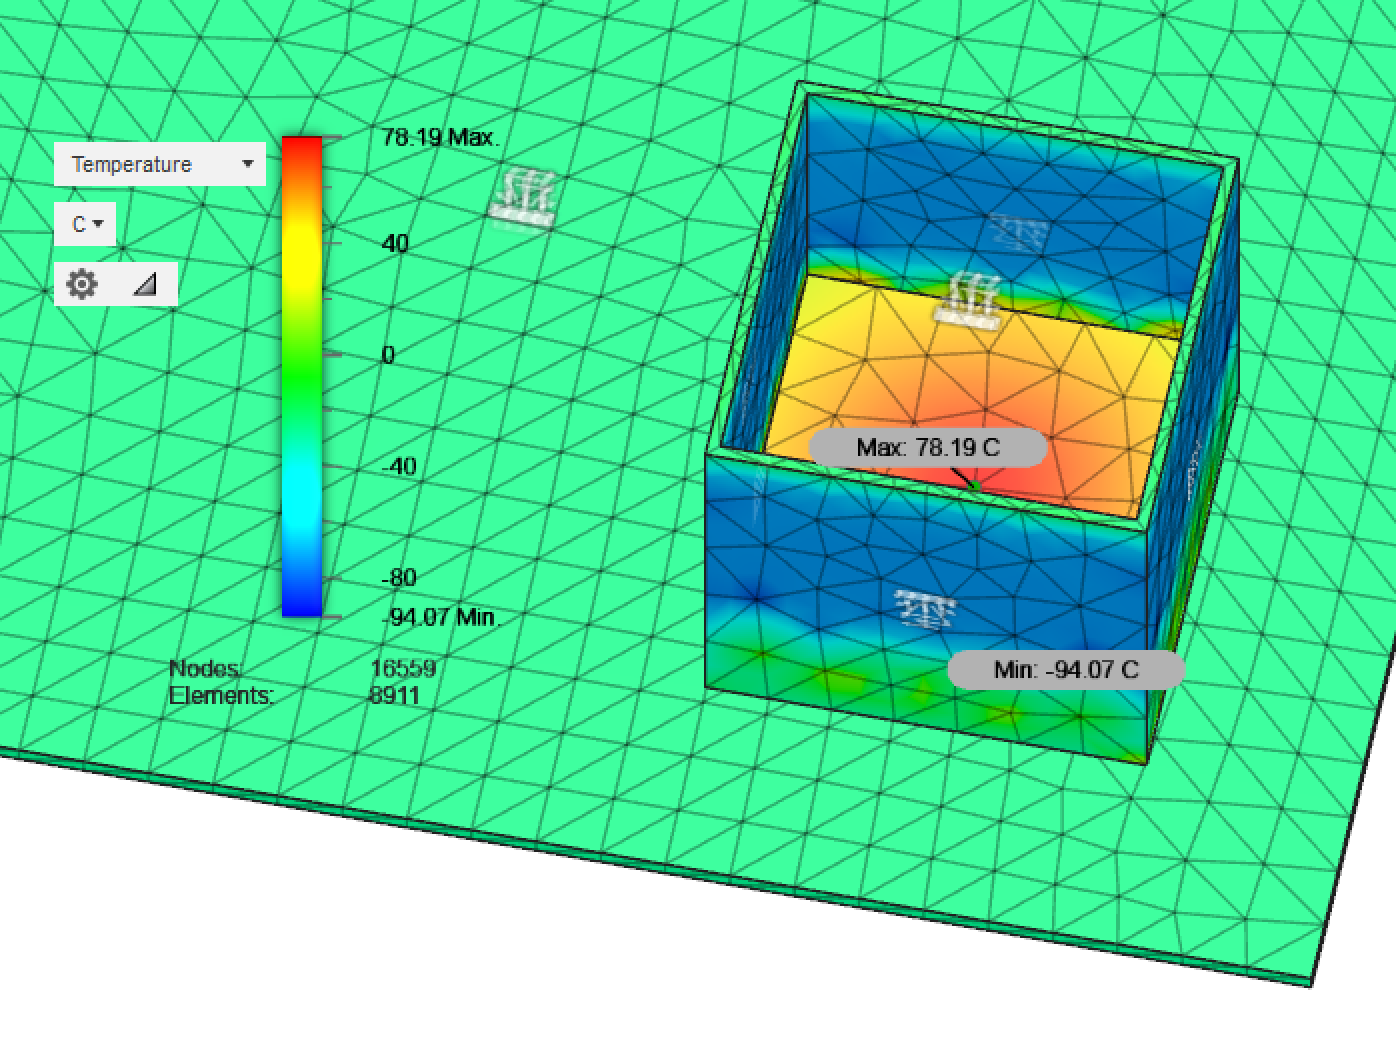
\includegraphics[scale=0.6]{4-experiment-design/img/mechanical/3mmthickheat.PNG}
	\caption{Thermal simulation of electronics box with 3mm insulation, exposed to solar heating.}
	\label{fig:3mmthickheat}
	\end{figure}

	\begin{figure}[H]
    \centering  
    \includegraphics[scale=0.65]{4-experiment-design/img/mechanical/1mmthickheat.PNG}
	\caption{Thermal simulation of electronics box with 1mm insulation, exposed to solar heating.}
	\label{fig:1mmthickheat}    
    	\end{figure}
    	
The 6mm insulation previously recommended yields a case where temperatures are too large, 134\textsuperscript{o}C compared to the required 50\textsuperscript{o}C maximum. This makes sense as the simplified 2D analysis did not account for the insulation material surrounding all edges of the PCB and did not account for solar heating. The thermal environment was also simulated assuming no solar heating for each insulation thickness, resulting in lower temperatures.\\

	\begin{figure}[H]
    \centering	
	\includegraphics[scale=0.58]{4-experiment-design/img/mechanical/6mmthicknoheat.PNG}
	\caption{Thermal simulation of electronics box with 6mm insulation, no solar heating.}
	\label{fig:6mmthicknoheat}
    	\end{figure}

	\begin{figure}[H]
    \centering    	
    \includegraphics[scale=0.6]{4-experiment-design/img/mechanical/3mmthicknoheat.PNG}
	\caption{Thermal simulation of electronics box with 3mm insulation, no solar heating.}
	\label{fig:3mmthicknoheat}
	\end{figure}

	\begin{figure}[H]
    \centering  
    \includegraphics[scale=0.65]{4-experiment-design/img/mechanical/1mmthicknoheat.PNG}
	\caption{Thermal simulation of electronics box with 1mm insulation, no solar heating.}
	\label{fig:1mmthicknoheat}    
    	\end{figure}
	
In this case 1mm insulation yields the best result with the temperatures at 38.2\textsuperscript{o}C with solar heating and -5\textsuperscript{o}C without, meeting the required temperatures for the electronics. It is important to note that this analysis also makes assumptions about perfect conductive interfaces and perfect distributions of material properties, as well as a fairly generic treatment of the thermal loads and geometry. Experimental testing will be required to ascertain more accurately the thermal conditions and to ensure that the thermal control that has been selected will work optimally and reliably.\\

Because of the use of polystyrene near the electrically charged PCBs, there is the possibility of electrostatic charging if the components are not secure or rub against each other. To ensure that this doesn't happen, the walls of the polystyrene box will be secured into place using non-conductive tape to achieve structural stability. The PCBs will also be attached so that there is an air gap between the PCB and the base and top of polystyrene box. Minimal contact between the PCBs and the insulation material will be a key factor during the assembly phase of the components.


\paragraph{Raspberry Pi heat sink}

It is also worth noting that in this analysis, the heat generated is distributed across the entire box instead of centralised in a smaller volume, which in reality would be the case as the Raspberry Pi generates most of the heat. This would result in much higher temperatures for the Raspberry Pi, possibly exceeding ideal temperatures. Indeed, measurements taken from previous experiments have indicated temperatures at the Raspberry Pi have exceeded 80\textsuperscript{o}C. A small heat sink should therefore be used to distribute the heat from the Raspberry Pi more evenly.\\ 

\paragraph{Reflecting tape for telescope}
An test was conducted to determine the effect of sudden temperature changes on the defocussing of the telescope, utilising spot lights as an analogy for the variation of solar radiation incident on the telescope. In this case the telescope was initially at equilibrium temperature of 21.5\textsuperscript{o}C, and a focusing target was placed 75 m from the telescope. For this experiment, temperature variations of up to 8\textsuperscript{o}C were recorded alongside the corresponding image captures. An obvious focus drift was recorded and attributed to geometric changes due to sudden thermal gradients on the telescope body and to a lesser extent on the mirrors.


	\begin{figure}[H]
    \centering	
	\includegraphics[scale=0.2]{4-experiment-design/img/mechanical/focusdrift.png}
	\caption{Defocussing of telescope for 6.3\textsuperscript{o}C temperature change.}
	\label{fig:focusdrift}
    	\end{figure}
 
In order to mitigate these sudden changes in temperature due to solar radiation, white tape will be used to cover the telescope body. This will increase the ratio of reflected radiation to absorbed so the changes in temperature become smaller.\\

Deformations occur not only due to random fluctuations in solar heating, but also due to the steady change of air temperature as the telescope is taken from its equilibrium temperature at 20\textsuperscript{o}C to -80\textsuperscript{o}C. The effect of this change on the optics can be estimated by using the principle of linear thermal expansion.

$\delta L = (L_0)(\alpha)(\delta T)$}

Where:

\begin{itemize}
  \item $\delta L$ is the change of length
  \item $L_0$ is the initial length
  \item $\alpha$ is the coefficient of linear thermal expansion
  \item $\delta T$ is the change of temperature
\end{itemize}


	\begin{figure}[H]
    \centering	
	\includegraphics[scale=0.58]{4-experiment-design/img/mechanical/mirrorgeometry.PNG}
	\caption{Properties of the main mirror.}
	\label{fig:mirrorgeometry}
    	\end{figure}
 
For the edges, the change of thickness is $\delta L = (17 mm)(0.000004 \frac{mm}{mm\textsuperscript{o}K}))(-100\textsuperscript{o}K) = 0.0068 mm$ The new thickness will be 17 mm - 0.0068 mm = 16.9932 mm.

For the center, the change of thickness is $\delta L = (17 mm)(0.000004 \frac{mm}{mm\textsuperscript{o}K}))(-100\textsuperscript{o}K) = 0.008 mm$. The new thickness will be 20 mm - 0.008 mm = 19.99200 mm.

This will affect the parabolic shape of the mirror, but not significantly. Unless indicated in further testing, it will be assumed that the deformation of the mirror due to the changing thermal environment is not a significant contributor to optical performance. To further isolate the mirror from other heat sources in the experiment and gondola, the mirror has been isolated by being mounted by three small screws that provide small conductive pathways. The conductive pathways are shown below.\\

	\begin{figure}[H]
    \centering	
	\includegraphics[scale=0.5]{4-experiment-design/img/mechanical/thermalpaths.PNG}
	\caption{Conductive pathways from the experiment to the mirrors.}
	\label{fig:thermalpaths}
    	\end{figure}


\paragraph{Heaters for motors and cameras}
The motors and cameras are distinct from the electronics box in that the power usage is much lower and so therefore the amount of heat able to be insulated is also lower. A simple estimate of the amount of insulation needed for the motors has been conducted using a rudimentary FEA model.\\

In this model, the motors are modelled as steel cylinders generating 0.91 W of heat, surrounded by extruded polystyrene, with outer surfaces losing heat by way of radiation and convection. The same thermal environment and material properties were used as in the analysis of the electronics box.\\

	\begin{figure}[H]
    \centering
    \includegraphics[scale=0.6]{4-experiment-design/img/mechanical/thermalmotors.PNG}
	\caption{Results of thermal analysis of motor with insulation and no sun shining.}
	\label{fig:thermalmotors}
	\end{figure}

It was found that in order to heat the motors to the required level, because of the small heat output, a 40 mm thick layer of insulation would be needed. This seems like a large requirement and will need to be verified with physical testing. If it is found that the amount of insulating material needs to be reduced for spatial, mechanical, or other reasons then the heating demands can still be met by adding in heating elements to the insulated environment, which would in effect increase the total "internal heat generation" and minimise the insulation requirement.\\

For these components Minco Polyimide Thermofoil heating pads can be used. These heating pads are able to increase the temperature of a target by up to 200\textsuperscript{o}C, more than enough to reach the required temperature range for the motors and cameras given the temperatures in the stratosphere.\\

Assuming all the heat is transferred directly to the component, the power can be related to the time required to increase the target temperature by a certain amount.

\begin{center}
 $P = \frac{mC_{p}(T_{f}-T_{i})}{t} $ \\
\end{center}

For the motors with a mass of 142\,g and made of steel with a specific heat of 0.50\,J/g/$^\circ$C, to raise the temperature by 10 degrees in 5 minutes we require 2.37 W of power. It is assumed that the camera is of similar properties. \\

\begin{center}
 $P = \frac{(142)(0.5)(10\textsuperscript{o}C)}{5(60)} = \SI{2.37}{W} $ \\
\end{center}

This can be related to the resistance of the required heating pad.

\begin{center}
 $P = \frac{V\textsuperscript{2}}{R} $\\

\end{center}

By selecting the pad with resistance 52.3\,$\Omega$ and running it at 10V, it will generate 1.91W of power, and will raise the temperature by 10 degrees in 6 minutes and 11 seconds.\\ 
 
This pad is the HK5165R52.3L12, capable of supplying 15W at 28V and has dimensions 25.4\,mm x 76.2\,mm.\\

Given that the components are to be maintained at 20\textsuperscript{o}C, the maximum allowable watt density can be found, after which overheating and burning of the heating pad will occur. This will help to determine the application method of the pad to the heat sink. \\

The area of the heater is 3\,inch$^2$. Dividing the power by this area yields a power density of 0.634\,W/inch$^2$.

	\begin{figure}[H]
    \centering
    \includegraphics[scale=0.8]{4-experiment-design/img/mechanical/wattdensity.JPG}
	\caption{The maximum allowable watt density for different application methods for a given heat sink control temperature. Source: Minco heaters}
	\label{fig:wattdensity}
	\end{figure}

As this is low burning of the heater is unlikely to occur unless the temperature is not properly regulated and the heating pad warms well beyond the desired control temperature. Also any application method is suitable with respect to this concern. To ensure proper conduction onto the surfaces of the motors and cameras, a thermal interface pad (ILA-TIM-CLUSTER-30X30-2A) will be used ensuring no air gaps that can cause spot heating or electric sparking. \\














\subsubsection{Thermal control}
The following methods for regulating the thermal environment have been suggested:

\begin{itemize}
  \item Extruded polystyrene to insulate electronics box self-heat.
  \item Heat sink for the Raspberry Pi in the electronics box.
  \item White reflecting tape, few conductive pathways for the telescope optics.
  \item Extruded polystyrene and Minco heaters to heat motors and cameras.

\end{itemize}

\begin{figure}[H]
\centering
\includegraphics[scale=0.8]{4-experiment-design/img/mechanical/thermalsolutions.png}
\caption{Summary of the thermal control mechanisms for the system.}
\label{fig:thermalsolutions}
\end{figure}

Risks have been identified and addressed including:

\begin{itemize}
  \item Electrostatic charging from movement of the polystyrene or PCBs.
  \item Overheating of the Raspberry Pi.
  \item Deformation of the mirrors.
  \item Air gaps between heaters and motors leading to spot heating.
  \item Air gaps between heaters and motors leading to electrical sparking.

\end{itemize}

To measure the temperature of the motors and especially cameras, which should be kept on the cooler end of the operating range, four Adafruit 165 temperature sensors will be used. This output will be fed into a simple proportional control loop to keep the components within the desired temperature range. Precision is not a major requirement for the thermal control.


\pagebreak
\subsection{Power System}

\label{sec:4.7}

A 28.8V (13 Ah) battery package can be provided by the gondola, according to the BEXUS user manual. One constrain is that the continuous maximum current is 1.8 A. Thus buck-converters will be needed to step down the voltage, while stepping up the current, so that the power needed will be delivered to the instrument. The voltage levels of the buck converters are: 

\begin{itemize}
	\item 28.8 V --> 3.3 V, with the power 1.65 W.
	\item 28.8 V --> 5 V, with power 15 W.
	\item 28.8 V --> 12 V, with power 15 W.
\end{itemize}

A schematic of the power system can be found in the appendix C.

The estimated power consumption of the components are shown in table \ref{tab: power consumption}. 
% import table of estimated power for components.

% highy recommend https://www.tablesgenerator.com/

\begin{center}
\begin{table}[H]
\begin{tabular}{|m{0.2\textwidth}|m{0.1\textwidth}|m{0.25\textwidth}|m{0.15\textwidth}|m{0.1\textwidth}|}
\hline
\textbf{Component Name} & \textbf{Supply Voltage {[}V{]}} & \textbf{Input Current {[}A{]} (MAX)} & \textbf{Power {[}W{]} (MAX)} & \textbf{Quantity} \\ \hline
Raspberry Pi CM3 Lite   & 5                               & 2                                   & 10                           & 1                 \\ \hline
DC Motors               & 12                              & 0.35                                & 4.2                          & 3                 \\ \hline
Gyroscope               & 3.3                             & 6.1m                                & 0.02013                      & 2                 \\ \hline
Magnetometer            & 3.3                             & 8m                                  & 0.0264                     & 1                 \\ \hline
GPS                     & 3.3                             & 10m                                 & 0.033                        & 1                 \\ \hline
Encoders                & 5                               & 8m                                  & 0.04                         & 2                 \\ \hline
Heater Motors           & 5                               & 0.188                               & 0.94                         & 3                 \\ \hline
Heater Camera           & 5                               & 0.382                               & 1.91                         & 1                 \\ \hline
Heater Electronics      & 5                               & 0.19                                & 0.95                         & 1                 \\ \hline
Camera                  & 5                               & 0.3                                 & 1.5                          & 1                 \\ \hline
Sanity Camera           & 3.3                             & 0.25                                & 0.825                        & 1                 \\ \hline
Guiding Camera          & 5                               & 0.3                                 & 1.5                          & 1                 \\ \hline
Accelerometer           & 3.3                             & 0.000155                            & 0.000558                     & 1                 \\ \hline
Temperature sensors     & 3.3                             & 1.5m                                & 0.00495                      & 5                 \\ \hline
Buck Converter 3.3V     & 28.8                            & 0.5(output)                         & 0.18333                      & 1                 \\ \hline
Buck Converter 5V       & 28.8                            & 3(output)                           & 1.6667                       & 1                 \\ \hline
Buck Converter 12V      & 28.8                            & 1.25(output)                        & 3.75                         & 1                 \\ \hline
\textbf{TOTAL}          & \textbf{-}                      & \textbf{4.946855}                   & \textbf{38.0099545}           &                   \\ \hline
\end{tabular}
\caption{The estimated power consumption of the components in active mode.}
\end{table}
\label{tab: power consumption}
\end{center}




\raggedbottom

\newpage

The BEXUS manual recommends the instrument to be prepared to have power supplies for 2 hours of testing, 2 hours on ground and for a flight time of 6 hours as a minimum. The instrument therefore needs to be in active mode for at least 8 h, because on ground the instrument will be in sleep mode. The instrument will also be in sleep mode for ascending and descending of the gondola. 

The total estimated power for the instrument:

\begin{itemize}
    \item Active mode: 38.02 W  --> 304 Wh (8h)
    \item Sleep mode: 15 W --> 45Wh (3h) 
\end{itemize}

Thus the instrument will require at least 349 Wh. The maximum power provided by the gondola will be 375 Wh, which should satisfy the instruments needs.


\raggedbottom

$  $\pagebreak
\subsection{Software Design}

\subsubsection{Purpose}

The purpose of the On-Board Software consists of:
\begin{itemize}
	\item Controlling the selecting and tracking of targets to observe.
	\item Ensuring that the camera is not oriented towards the sun.
	\item Reading data from sensors and controlling actuators when needed.
	\item Processing and storing images taken by camera.
	\item Logging housekeeping data.
	\item When possible, sending images and housekeeping data to ground station.
\end{itemize}

The software is designed such that it can control the experiment autonomously throughout the whole experiment process but also enable control from ground through telecommands.

\subsubsection{Design}
\label{sec:4.8.2}

\paragraph{a)} Process Overview

\begin{figure}[H]
	\centering
	\includegraphics[width=.9\textwidth]{4-experiment-design/img/software/process-overview.png}
	\caption{Relations between On-Board Computer and connected components.}
	\label{fig:software-process-overview}
\end{figure}

All external components connected to the On-Board Computer and their interface are displayed in figure \ref{fig:software-process-overview}. The sanity camera provides an overview of the experiment and captures images on demand. The guiding camera provides an overall view in the direction the telescope is pointing and is also used as a star tracker to determine the gondola attitude. \st{A secondary microcontroller will be used to support the high sampling frequency needed for the gyroscopes. This microcontroller will be polled by the OBC.}

\paragraph{b)} General and safety related concepts

To ensure that the software is not erroneous rigorous testing will be done during development and after completion. A watchdog timer will be used to avoid software freezing. This timer will reset the On-Board Computer if it is not itself reset by the software within a certain period.

\paragraph{c)} Interfaces

If connection to ground is available, images compressed with a lossless compression will be sent down over the E-link over the course of the experiment. If the storage were to fail on touchdown for any reason, this would mean that not all data is lost. All communications over the E-link will be done using TCP to ensure that packet loss won't corrupt data.

\begin{table}[H]
	\centering
	\begin{tabular}{l|l}
		\textbf{Component}
		& \textbf{Interface} \\ \hline
		Ground Station
		& E-link             \\
		NIR Camera
		& USB                \\
		Guiding Camera
		& USB                \\
		Gondola GPS
		& SPI                \\
		Telescope Gyroscope
		& I2C                \\
		Telescope Encoders
		& I2C                \\
		Controller Actuators
		& I2C                \\
		Thermal Sensors
		& I2C				 \\
		Heaters \& Coolers
		& I2C
	\end{tabular}
	\caption{Table showing the interface that each external component was connected with. This is also visually represented in figure \ref{fig:software-process-overview}.}
	\label{tab:software-interfaces}
\end{table}


All housekeeping data will be stored in the form of text documents. This data will be transmitted to ground periodically. In the beginning of observations, images from the guiding camera will also be transmitted to verify that the system is working as intended. In the case that the images from the guiding camera are not as expected, an image from the sanity camera can be transmitted on demand. This is the only case a sanity image would be transmitted.

So long as there is additional headroom in the link budget, images from the NIR camera will be transmitted to ground. How many and when images are transmitted as well as an upper limit on the data rate if needed shall be controlled from ground. A minimum bandwidth of 300\,kbit/s is required for sensor data and guiding images. Once the initial guiding images has been received and verified, the nominal bandwidth required to transmit 10 images per hour is 500\,kbit/s. Any available bandwidth above that can be used to transmit additional images.

\newpage
The telecommands are very small compared to the telemetry. In the worst case scenario the command size is in the kbit range after all communication overhead is added. The following points shall be controllable from the ground station:

\begin{itemize}
	\item Rebooting the entire system.
	\item Updating the list of targets and their priorities.
	\item Calibrating the tracking to remove any offsets that may have appeared.
	\item Choosing how fast and how many NIR images will be transmitted.
	\item Setting camera settings such as exposure time and sensor gain.
	\item On-command image capturing with the guiding or sanity cameras.
\end{itemize}

\paragraph{d)} Data acquisition and storage

All data will be compressed using zstd, a lossless compression. The resulting compression ratio is heavily dependent on the contents of the data. A ratio of 2:1 (original data size to compressed) is used as a rough estimate from testing.

The main bulk of data handled is the images taken by the cameras. Housekeeping data such as positioning, camera direction, time, etc will also be stored along with the images. The On-Board Computer has one SD card used for the OS and temporary storage. For the external data storage two SD cards are used for redundancy purposes. All data shall be saved on these external SD-cards.

Both the NIR camera and the guiding camera have a colour depth of 12\,bits, but the image file format demands 16\,bits\,per\,pixel. This results in extra zero-padding on the data. However as this appears regularly, the compression algorithm can easily reduce the size overhead greatly.

As the NIR camera has a resolution of $5496 * 3672$ and 16\,bits\,per\,pixel, the raw image compressed size will be roughly 20\,MB. For a 4\,hour float phase and an exposure time of 30\,s a total of  9.69\,GB is required in on-board data storage for the images. An exposure time of 30\,s can't be guaranteed e.g. due to movements of the gondola. If the exposure time is dropped to 10\,s the total amount of data for continuous image capturing is 29\,GB.

The guiding camera has a resolution of $1936 * 1096$ and 16\,bits\,per\,pixel, leading to a raw image compressed size of roughly 2.1\,MB. If the guiding camera is sampled every 10\,s the total data required for the images is 3\,GB.

As the housekeeping data is negligible in size compared to the images and as the sanity images are only taken on demand, an SD-card size of 64\,GB will be sufficient for all data storage.

With a maximum of 1\,Mbit per second data transfer rate to ground it takes at least 161.5\,s to transfer one image compressed losslessly to 50\,\% of original size. This means that with little down time between observations and for most exposure times, not all images can be transmitted to ground.

The minimum data rate to the external storage required to save NIR images every 30\,s, guiding camera images every 10\,s, and sensor data polled each second is 900\,kbit/s.


\paragraph{e)} Process Flow

The system can either start in a testing mode, or in normal operation. The testing mode is used for pre-flight tests to ensure that all systems work as expected. Afterwards the system shall enter a sleep mode, a low activity state, with the camera in a safe launch position. During the ascent the thermal control system shall be running to ensure that all components of the experiment are within nominal temperature ranges.

When the float phase is reached, the system will wake. This is done by tracking the altitude of the gondola using GPS data. After wake-up the system shall find its orientation and the position of the sun. Finally tracking and observation can start.

Astronomical targets are prioritised. The software shall track and observe the highest priority target within the field of view with varying camera settings until one of the following events happen:

\begin{itemize}
	\item Current target leaves operational field of view.
	\item \st{Target moves too close to the sun for observation.}
	\item A higher priority target enters the field of view.
\end{itemize}

If one of the aforementioned events happens, the software will switch current target following prioritisation. While observing targets, the On-Board Software shall store images and housekeeping data. If connection to ground is available this data shall be compressed using a lossless compression method and sent to ground.

At the end of the floating phase the camera shall be oriented in a landing position and the system shall shut down. Figure \ref{fig:software-activity-diagram} shows the complete process flow. Figure \ref{fig:software-state-diagram} shows a simple state diagram for the experiment. Observations are done in the Normal state. In the rare case of a software freeze, it will be reset without entering sleep mode.

\begin{figure}[H]
    \centering
    \includegraphics[width=.5\textwidth]{4-experiment-design/img/software/activity-diagram.png}
    \caption{Activity diagram describing the complete software flow. Here the internal actions SOE and EOE refer to when the software starts, i.e. on the launch pad, and shuts down respectively. This is done independently and therefore requires no activity from the gondola.}
    \label{fig:software-activity-diagram}
\end{figure}

\begin{figure}[H]
	\centering
	\includegraphics[width=.7\textwidth]{4-experiment-design/img/software/state-diagram.png}
	\caption{State diagram for On-Board Software.}
	\label{fig:software-state-diagram}
\end{figure}

\clearpage
\paragraph{f)} Modularisation and pseudo code

\begin{figure}[H]
	\centering
	\includegraphics[width=\textwidth]{4-experiment-design/img/software/composition-tree.png}
	\caption{Composition tree of On-Board Software. \hl{[Updated figure]}}
	\label{fig:software-composition-tree}
\end{figure}

Figure \ref{fig:software-composition-tree} shows how the complete software is modularised. Each component is described below.

\begin{itemize}

	\item Camera: Parent
		\begin{itemize}
			\item \st{Camera Control: Module responsible for selecting target, camera settings and capturing images.}
			\item Guiding Camera: Communication link to the guiding camera.
			\item NIR Camera: Communication link to the NIR camera.
			\item Sanity Camera: Communication link to the sanity camera.
		\end{itemize}

	\item Command: Module responsible for handling incoming commands from ground.

	\item \st{Data Storage: Module providing an interface to store data to the external SD-cards.}

	\item E-link: Module responsible for communications over the E-link interface.

    \item \hl{GPIO: Module responsible for communications through the Raspberry Pi GPIO.}

	\item \st{I2C: Module responsible for communications over the I2C bus.}

	\item Img Processing: Image processing, parent
		\begin{itemize}
			\item Data Queue: Buffer to hold camera data until Handler is ready
			\item Image Handler: Module processing and storing images taken by camera.
		\end{itemize}

	\item Init: Module initialising each component.

	\item Mode: Module responsible for the current state of the software.

	\item Sensors: Parent
		\begin{itemize}
            \item \hl{Encoder: Module holding encoder data.}
            \item \hl{GPS: Module holding GPS data.}
            \item \hl{Gyroscope: Module holding gyroscope data.}
			\item \st{Orientation: Module keeping track of orientation and location.}
			\item \st{Sun: Module keeping track of position of the sun.}
			\item Sensor Poller: Module responsible for polling sensors.
            \item \hl{Star Tracker: Module holding absolute attitude obtained from the star tracker.}
			\item Temperature: Thermal sensors.
		\end{itemize}

	\item \st{SPI: Module responsible for communications over the SPI bus.}

	\item Telemetry: Parent
		\begin{itemize}
			\item Downlink: Module responsible for sending telemetry to ground.
			\item Downlink Queue: Buffer to hold telemetry messages.
		\end{itemize}

	\item Thermal: Module responsible for active thermal control

	\item \hl{Control System} \st{Tracking}: Parent
		\begin{itemize}
			\item Current Target: Module holding the current target to be observed.
			\item \hl{Stabilisation} \st{Controller}: Module responsible for keeping camera on target.
			\item Gimbal: Module providing an interface to the gimbal motors.
			\item Target \hl{Selection} \st{Choosing}: Module responsible for keeping track of target prioritisation \hl{and positioning as well as controlling the main camera}.
		\end{itemize}

	\item Watchdog: Timer to reset \st{external} watchdog.

\end{itemize}

\subsubsection{Implementation}

The code for the On-Board Software shall be implemented in C. An operating system will be used to enable the modularisation required. The chosen operating system is Linux with the Preempt RT kernel patch. Additional libraries, such as the ASI SDK library used for controlling the cameras, will be needed. The compression used for the telemetry is supplied by the zstd library.



\subsubsection{Control system}
The main task of the control system is selecting and tracking the astronomical targets and stabilising the telescope during exposure. Other tasks include minor tasks like the thermal control of the CMOS sensor and the electronics box as well as control of the actuators. A general overview of the control loop for tracking \& stabilisation is given in figure  \mbox{\ref{fig::software::control_loop}} below. The thermal control loop is sketched in chapter \mbox{\ref{Thermal_section}}.

\paragraph{Selecting and tracking targets}

The selection and tracking of targets is done by using the current time, position (GPS) and orientation star tracker and gyroscope) of the gondola. Once a suitable target in the operational field of view is selected, it is tracked during exposure. This includes the compensation of the following motions:
\begin{itemize}
	\item Time-dependent rotational motion of the astronomical targets in the sky. This will be continuously compensated during exposure using models and/or interpolation of tables.
	\item Position-dependent rotational motion of the astronomical targets in the sky. This will be corrected once for every picture, using the GPS data.
	\item Rotation of the gondola in the z-axis; can be corrected during exposure using a gyroscope sensor.
\end{itemize}

Due to the nature of the motion of astronomical targets, it is necessary to use a 3-axis gimbal.

The three axes and the names for the rotation axes are shown in figure \mbox{\ref{fig::software::Yaw_Pitch_Roll}}.

\textbf{Selection of targets}

The selection of targets is based on the operational field of view (the area of the sky where the telescope is able to look at) and prioritisation parameters of the possible targets within this field of view. The operational field of view is determined by using the sensor data from the orientation sensor (star tracker). Using a star tracker will provide an accurate absolute attitude determination system to ensure that the celestial object of interest is actually in the field of view of the telescope when it is pointed there. Compared to the gyroscopes that have a much higher angular resolution, the attitude determination system does not show any drift over time and does therefore not need to be calibrated during flight.

Prioritisation parameters include the brightness of the object (brighter objects are expected to yield better results due to higher SNR), the location of the object within the operational field of view (objects near the centre of the field of view are favoured because they are less likely to rotate out of the field of view during exposure) and the number of exposures already taken (objects should be imaged more than once in order to be able to compare and verify the obtained data, but not more often than ten times during the flight). 

As the location of the astronomical targets changes with time and position of the gondola, these two parameters also need to be taken into account (for determination see paragraph Astronomical targets). Once a target is selected, this part of the control system will be deactivated until the picture was taken or the control loop is re-initialised.

\hl{The 4 chosen prioritisation parameters are: }
\begin{itemize}
	\item \hl{No. of exposures already taken (exposure parameter)}
	\item \hl{Magnitude of the target (constant)}
	\item \hl{Position parameter}
	\item \hl{Type of target  (defined scientific parameter, constant)}
\end{itemize}

\hl{The exposure parameter depends on the number of images of the target that have already been taken, and is defined as follows: \texttt{exp\_ param\_ list = [1,2,3,4,4,4,3,2,1,1,1]} for 0 to 9 exposures respectively, and 0 for all other. This ensures that not more than 10 images are taken (maximum defined in the scientific requirements) and that targets with more than 2 exposures are prioritised in order to get sufficient scientific data of one target.
}

\hl{The magnitude of the target is defined by the target itself and is therefore constant. Typical values range from 3 to 10 for the chosen targets. The higher the value the brighter the target, and therefore more suitable to observe.
}

\hl{The position parameter depends on the gondola attitude and is recalculated based on the current time, position and attitude each time. It is then calculated as follows: if the absolute difference between the gondola attitude and the target position is smaller than a set value (e.\,g.~maximum telescope range - $\ang{30}$) it is defined as 
}
\begin{align*}
	\left|\text{gondola attitude} - \text{target position} \right|
\end{align*}
\hl{otherwise as zero. This means that no targets that are outside the field of view are chosen, and the most central targets are preferred in order to minimise the risk of the target rotating out of the field of view during exposure.
}

\hl{The type of target (nebula/galaxy/open cluster/globular cluster) prioritises nebulae and galaxies to cluster. The prioritisation order is \texttt{type\_ param\_ list = [4,3,2,1]} for the order mentioned above.
}

\hl{To get a final prioritisation value for each target, all prioritisation parameters are multiplied. This ensures that targets outside the field of view as well as targets with 10 exposures are not taken into consideration any more, as the result is 0. The target with the highest calculated prioritisation value is selected for the next exposure.
}



\textbf{Tracking of astronomical targets}

The time-dependent and the position-dependent rotational motion of the astronomical targets are calculated by using an astronomical model and provides the control input for the subsequent stages of the control system. Because the state vectors for this model are time (internal clock) and position (GPS) and the input vector is the selected target (defined in the system, not a variable state for the exposure of one image), the state vectors cannot be affected by the control system (not controllable). Therefore, no dedicated feedback loop is used for this part of the control system. However, the input data from the GPS may be filtered before use. The output vector then provides the input for the compensation of rotation (of the gondola in the z-axis) and the stabilisation of the gimbal.

\hl{The astronomical model used to determine the current position of the targets is the Alt Az (Altitude Azimuth) reference frame. It defines the position of the astronomical target with respect to geographic north and zenith and depends on current the time, date and position of the observer. It is calculated based on the RA DEC (Right Ascension, Declination) of the astronomical target. The formulas required for this conversion are given in \mbox{\cite{RaDec2AltAz}}.
}

\textbf{Rotation of the gondola}

The uncontrolled rotational motion of the gondola around the z-axis can be directly compensated by actuating the corresponding gimbal axis (yaw). This will be achieved by a PID control. As the same axis will also be actuated during the stabilisation process, it will be merged with the control loop for the stabilisation. As the required accuracy for detecting the rotation of the gondola is very high, the gyroscopes are used to provide the input (see stabilisation for more detail).


\paragraph{Stabilisation of the gimbal}
The stabilisation of the gimbal only needs to be active during exposure in order to avoid blurred pictures. It is responsible for compensating all kinds of small-scale, unpredicted movements of the gondola. In order to achieve this, an active feedback loop that requires information about the gondola movements is needed. This information is gathered by using accelerometers and gyroscopes for all 3 axes.

After the target is selected, the gyroscopes are reset so there is no offset-error and the best accuracy can be achieved. With this setup, it is possible to measure the movements of the gondola with an accuracy higher than the corresponding angular resolution of one pixel. Once the gyroscopes are reset the value of the attitude determination system is held constant within the control system, because the accuracy of the gyroscopes is orders of magnitude higher than that of the attitude determination system. 

In addition to the gyroscopes, the encoders are used to obtain the actual position of the telescope within the gondola and therefore provide a second set of data for the feedback loop. The sensor data is filtered by a Kalman filter to decrease the sensor noise and deduce the current orientation of the telescope as well as the motion of the gondola with a high precision.

The control of the gimbal (tracking and stabilisation as well as compensation of the gondola rotation for the yaw axis) is done by a separate PID control for each axis. The output of the controller is the required speed for the actuating motor of the respective axis. This information is then processed by the motor controller that calculates the required input currents for the motors.

\hl{The stabilisation algorithm is written in C as the most of the OBSW. The team refrained from using third party libraries, so the whole stabilisation code is built using standard C libraries. The analisys will be conducted on a Simulink model and acquired PID values are tested on an instrument during integration tests.}

%\begin{figure}%[h]
%	\centering
%	\includegraphics[width = 0.4\textwidth]{4-experiment-design/img/software/Yaw_Pitch_Roll.eps}
%	\caption{\hl{Yaw, Pitch and Roll angles of the gimbal [New figure]}}
%	\label{fig::software::Yaw_Pitch_Roll}
%\end{figure}

\newpage
\begin{landscape}
	\begin{figure}
		\includegraphics[width=\linewidth]{4-experiment-design/img/software/Control_loop.eps}
		\caption{Control loop of the experiment}
		\label{fig::software::control_loop}
	\end{figure}
\end{landscape}


\raggedbottom

\pagebreak
\subsection{Ground Support Equipment}\label{sec:4.9}
A laptop on the ground was connected to the experiment via the E-Link. A spare laptop was kept close-by should any problems arise with the main one. The ground support software included a simple GUI which enabled an operator to issue commands to the experiment such as reset, target selection, and moving to landing position. Compressed pictures could be received by the ground support software, which could be examined to verify nominal operation. The ground support software was written in C and Python, using GTK+ to build the GUI.

\begin{figure}[h]
	\centering
	\includegraphics[width=\textwidth]{4-experiment-design/img/software/GSS-tree.png}
	\caption{Design tree of IRISC Ground Support Software}
	\label{fig:gss-tree}
\end{figure}

The ground support software that was running is shown in figure \ref{fig:gss-tree}. The RXTX object sent and received data via the E-link. The INIT object initialized the software. The COMMAND object read and parsed commands sent by the user through the GUI, which would also be used by the DISPLAY object to show received data to the user. The SAVE object was used to save the received data to local storage, and lastly the MODE object handled the modes of the software.
\raggedbottom

\raggedbottom
\pagebreak
\section{Experiment Verification and Testing}

\subsection{Verification Matrix}

The verification matrix is made following the standard of \textit{ECSS-E-10-02A}. \cite{ECSSSecretariat}.  

\textit{There are four established verification methods:}
\newline \textit{A - Verification by analysis or similarity}
\newline \textit{I - Verification by inspection}
\newline \textit{R - Verification by review-of-design}
%\newline \textit{S - Verification by similarity}
\newline \textit{T - Verification by testing}

% https://www.tablesgenerator.com/ highly recommended.

\makeatletter
\renewcommand\@makefntext[1]{\leftskip=3em\hskip-1em\@makefnmark#1}
\makeatother

\begin{longtable}[]{|m{0.05\textwidth}| m{0.41\textwidth}|m{0.11\textwidth}|m{0.11\textwidth}|m{0.11\textwidth}|m{0.11\textwidth}|}

\hline
\textbf{ID} & \textbf{Requirement text} & \textbf{Method} & \textbf{Reference} & \textbf{Status} & \textbf{Verifica-tion result} \\\hline

\rowcolor{yellow} F.3 & The system shall be able to find the celestial objects of interest at the location and orientation of the gondola.
& ??? & Tests: ??? & A: to be done \newline T: to be done & Not verified \\\hline

\rowcolor{yellow} F.4 & The system shall be able to orient towards selected celestial objects of interest.
& ??? & Test: ??? & R: to be done & Not verified \\\hline

\rowcolor{yellow} F.5 & The system shall be able to counter balance perturbations of the gondola during exposure.
& ??? & Test: ??? & R: to be done & Not verified \\\hline

\rowcolor{yellow} F.6 & The camera and optics system shall be able to record the selected celestial object of interest.
& ??? & Test: ??? & R: to be done & Not verified \\\hline




P.2 & The optics shall be cable of making pictures of 0.5-1.5 x 0.3-1\,degrees.
& R, T & Test: 1 & R: to be done \newline T: to be done & Not verified \\\hline

P.3 & The NIR camera shall make images in the range of 720-850 to 1200\,nm.
& R & Test: 1 & R: to be done & Not verified \\\hline

P.4 & The NIR camera shall have a resolution of at least 16\,MP.
& R, T & Test: 1 & R: to be done \newline T: to be done & Not verified \\\hline

%TODO : MODIFIED!
P.5 & The NIR camera shall be able to take pictures with an exposure time up to 30\,seconds.
& R, T & Test: 1 & R: to be done \newline T: to be done & Not verified \\\hline

P.6 & The NIR camera shall be able to take pictures with an exposure time up to 30\,seconds.
& R, T & Test: 1 & R: to be done \newline T: to be done & Not verified \\\hline

P.7 & The NIR camera shall be able to take pictures with an exposure time up to 30\,seconds.
& R, T & Test: 1 & R: to be done \newline T: to be done & Not verified \\\hline

P.8 & The NIR camera shall be able to take pictures with an exposure time up to 30\,seconds.
& R, T & Test: 1 & R: to be done \newline T: to be done & Not verified \\\hline

\rowcolor{yellow} P.9 & The system shall be able measure the orientation of the gondola with an accuracy of 0.5 degree.
& ??? & Test: ??? & R: to be done \newline T: to be done & Not verified \\\hline

\rowcolor{yellow} P.10 & The system shall be able measure the position of the gondola with an accuracy of 5 meters.
& ??? & Test: ??? & R: to be done \newline T: to be done & Not verified \\\hline

\rowcolor{yellow} P.11 & The pointing error of the guiding camera in relation to the NIR camera shall be less than 0.35 degrees.
& ??? & Test: ??? & R: to be done \newline T: to be done & Not verified \\\hline

\rowcolor{yellow} P.12 & The temperature of the NIR camera shall be held between -5 and 0\,$^\circ$C during operation.
& ??? & Test: ??? & R: to be done \newline T: to be done & Not verified \\\hline

\rowcolor{yellow} P.13 & The temperature of the NIR camera should be held between -5 and -3\,$^\circ$C during operation.
& ??? & Test: ??? & R: to be done \newline T: to be done & Not verified \\\hline

\rowcolor{yellow} P.14 & The temperature of the rotating part shall be held between 0 and 85\,$^\circ$C.
& ??? & Test: ??? & R: to be done \newline T: to be done & Not verified \\\hline

\rowcolor{yellow} P.15 & The temperature of the electronics shall be held between -40 and 85\,$^\circ$C.
& ??? & Test: ??? & R: to be done \newline T: to be done & Not verified \\\hline



D.01 & The experiment shall be able to operate in the temperature profile of the BEXUS environment.
& T & Test: 2 & T: to be done & Not verified \\\hline

D.02 & The experiment shall be able to operate in the pressure profile of the BEXUS environment.
& T & Test: 2  & T: to be done & Not verified \\\hline

D.03 & The experiment shall be able to operate in the vibration profile of the BEXUS environment.
& T & Tests: 8, 10 & T: to be done & Not verified \\\hline

D.05 & The supporting structure shall not twist by more than 0.1\,degrees.
& T & Tests: 9, 10 & T: to be done & Not verified \\\hline

D.07 & The experiment shall be able to fly during the entire day.
& T & Tests: 9, 10 & T: to be done & Not verified \\\hline

D.10 & The experiment shall be mounted at the side of the gondola.
& T & Tests: 9, 10 & T: to be done & Not verified \\\hline

D.11 & The experiment shall not consume more power than 250\,Wh.
& T & Tests: 9, 10 & T: to be done & Not verified \\\hline

D.13 & The mass of the experiment shall not exceed 20\,kg.
& I & Test: 7 & I: to be done & Not verified \\\hline

D.14 & The experiment shall be able to run for at least 2.5\,hours.
& T & Tests: 9, 10 & T: to be done & Not verified \\\hline

D.15 & The experiment shall be able to function autonomously.
& T & Tests: 4, 9, 10 & T: to be done & Not verified \\\hline

D.16 & The data stored in the experiment shall be able to survive the landing.
& T & Test: 8 & T: to be done & Not verified \\\hline

\rowcolor{yellow} D.17 & The data stored in the experiment shall be able to survive the landing.
& ??? & Test: ??? & T: to be done & Not verified \\\hline

\rowcolor{yellow} D.18 & The images obtained shall be sent to a ground station by the E-link system with a various and adjustable datarate between 250 and 1000 kilo bits per second.
& ??? & Test: ??? & T: to be done & Not verified \\\hline




O.1 & The experiment shall be able to be controlled by the ground station when requested.
& T & Tests: 4, 10 & T: to be done & Not verified \\\hline

O.2 & The experiment shall rotate to a 'safe' position while descending.
& T & Tests: 4, 9, 10 & T: to be done & Not verified \\\hline

\rowcolor{yellow} O.3 & The telescope shall not be pointed within 27\,degrees of the sun.
& ??? & Tests: ??? & T: to be done & Not verified \\\hline

\caption{Verification Matrix.}
\label{tab:var-mat}
\end{longtable}
\raggedbottom

\pagebreak
\subsection{Test Plan}

\subsubsection{Planned Tests}
The planned tests are as follows:

\begin{enumerate}[leftmargin=2.1cm]
   \item[Test 01:] Optics \& Camera;
   \item[Test 02a:] Thermal test;
   \item[Test 02b:] Pressure test;
   \item[Test 03:] Electronics;
   \item[Test 04:] Software with electronics;
   \item[Test 05:] Control system;
   \item[Test 06:] Data transfer;
   \item[Test 07:] Mass;
   \item[Test 08:] Drop test (without optics and camera);
   \item[Test 09:] Gimbal mounted on replicated gondola;
   \item[Test 10:] Gimbal mounted on a car;
   \item[Test 11:] Sun avoiding.
   \item[Test 12:] Analyses of components.
\end{enumerate}

\subsubsection{Test Descriptions}

\begin{table}[H]
\centering

\begin{tabular}{|m{0.3\textwidth}| m{0.7\textwidth} |}
\hline
\textbf{Test Number} 	& 1 					\\ \hline
\textbf{Test Type} 		& Optics \& Camera  	\\ \hline
\textbf{Test Facility} 	& LTU (outside), Kiruna \\ \hline
\textbf{Tested Item} 	& Optics \& Camera 		\\ \hline

\multirow{2}{*}{\textbf{\begin{tabular}[c]{@{}l@{}}Test Level/ Procedure \\ and Duration\end{tabular}}}
& Verify the design that pictures are only able to be made in the specified NIR spectrum range, with the specified resolution and angular size. Then put the selected optics with camera on a tripod and obtain images of all the selected targets. For these tests the NIR filter may be temporarily removed (if possible). But all targets should be photographed at least in the NIR spectrum.
\\ & Test duration: 8 hours (at night). \\ \hline

\textbf{Test Campaign Duration} 	& 1 day 	\\ \hline
\textbf{Test Campaign Date} 		& September		\\ \hline

\textbf{Test Completed} 			& YES 		\\ \hline
\textbf{Requirements verified}		& PARTIALLY: Test was done without tripod nor IR filter 		\\ \hline
\end{tabular}
\caption{Test 1: Optics \& camera ground tested.}
\label{tab:test1:optics-and-camera}
\end{table}


\raggedbottom


\begin{table}[H]
\centering

\begin{tabular}{|m{0.3\textwidth}| m{0.7\textwidth} |}
\hline
\textbf{Test Number} 	& 2a 					\\ \hline
\textbf{Test Type} 		& \st{Vacuum \&} Freezer		\\ \hline
\textbf{Test Facility} 	& IRF/ EISCAT, Kiruna 	\\ \hline
\textbf{Tested Item} 	& Electronics, optics and camera \\ \hline

\multirow{2}{*}{\textbf{\begin{tabular}[c]{@{}l@{}}Test Level/ Procedure \\ and Duration\end{tabular}}}
& The electronics, optics and camera should be placed in \st{a vacuum and} freezer to test the components functionality with a simulated environment based on the one we expect to encounter. The \st{pressure should be <5\,mbar and} temperature -80\,$^\circ$C (or atleast colder than -40\,$^\circ$C if not possible) The components may be tested separately, but should function during the test.
\\ & Test duration: 15 minutes per test on the specified pressure and temperature. \\ \hline

\textbf{Test Campaign Duration} 	& 1 day 	\\ \hline
\textbf{Test Campaign Date} 		& Beginning of June	\\ \hline

\textbf{Test Completed} 			& NO 		\\ \hline
\textbf{Requirements verified}		& NO 		\\ \hline
\end{tabular}
\caption{Test 2a: \st{Vacuum and} Freezer test of at least the electronics, optics and camera.}
\label{tab:test2:vacuum}
\end{table}


\raggedbottom

\begin{table}[H]
\centering

\begin{tabular}{|m{0.3\textwidth}| m{0.7\textwidth} |}
\hline
\textbf{Test Number} 	& 2b 					\\ \hline
\textbf{Test Type} 		& Vacuum		\\ \hline
\textbf{Test Facility} 	& IRF/ EISCAT, Kiruna 	\\ \hline
\textbf{Tested Item} 	& Electronics, optics and camera \\ \hline

\multirow{2}{*}{\textbf{\begin{tabular}[c]{@{}l@{}}Test Level/ Procedure \\ and Duration\end{tabular}}}
& The electronics, optics and camera should be placed in a vacuum to test the components functionality with a simulated environment based on the one we expect to encounter. The pressure should be <5\,mbar. The components may be tested separately, but should function during the test.
\\ & Test duration: 15 minutes per test on the specified pressure. \\ \hline

\textbf{Test Campaign Duration} 	& 1 day 	\\ \hline
\textbf{Test Campaign Date} 		& Beginning of June	\\ \hline

\textbf{Test Completed} 			& NO 		\\ \hline
\textbf{Requirements verified}		& NO 		\\ \hline
\end{tabular}
\caption{Test 2b: Vacuum test of at least the electronics, optics and camera.}
\label{tab:test2:vacuum}
\end{table}


\raggedbottom


\begin{table}[H]
\centering

\begin{tabular}{|m{0.3\textwidth}| m{0.7\textwidth} |}
\hline
\textbf{Test Number} 	& 3 				\\ \hline
\textbf{Test Type} 		& Electronics		\\ \hline
\textbf{Test Facility} 	& LTU, Kiruna 		\\ \hline
\textbf{Tested Item} 	& Sensors and Actuators	\\ \hline

\multirow{2}{*}{\textbf{\begin{tabular}[c]{@{}l@{}}Test Level/ Procedure \\ and Duration\end{tabular}}} 
& The sensors should first be read out one by one, without the other sensors connected. If multiple sensors or actuators are located on the same PCB, there should also be a test PCB available with each sensor and actuator separated from the prototype phase. Afterwards, the same is done for each actuator. Then, one by one, each sensor and actuator is added to the system to test the system as a whole. 
\\ & Test duration: 5 hours. \\ \hline

\textbf{Test Campaign Duration} 	& 1 day 	\\ \hline
\textbf{Test Campaign Date} 		& Beginning of October	\\ \hline

\textbf{Test Completed} 			& YES 		\\ \hline
\textbf{Requirements verified}		& YES 		\\ \hline
\end{tabular}
\caption{Test 3: Sensors and actuators test.}
\label{tab:test3:electronics}
\end{table}


\raggedbottom

\begin{table}[H]
\centering

\begin{tabular}{|m{0.3\textwidth}| m{0.7\textwidth} |}
\hline
\textbf{Test Number} 	& 4 				\\ \hline
\textbf{Test Type} 		& Software 			\\ \hline
\textbf{Test Facility} 	& LTU, Kiruna 		\\ \hline
\textbf{Tested Item} 	& Raspberry pi software with electronics connected. \\ \hline

\multirow{2}{*}{\textbf{\begin{tabular}[c]{@{}l@{}}Test Level/ Procedure \\ and Duration\end{tabular}}}
& This test should be done after the functionality of the electronics is verified. Then all sensors and actuators should be tested integrated with the software. Let the gimbal be targeting 4 specific points with a separation of 90 degrees. Test if the gimbal stabilize the system when moved and switches targets based on the field of view. The targets should also be able to be switched on the ground station. Then add a 5th target which it may never look directly at and repeat the test.
\\ & Test duration: 5 hours. \\ \hline

\textbf{Test Campaign Duration} 	& 1 day 	\\ \hline
\textbf{Test Campaign Date} 		& Beginning of June	\\ \hline

\textbf{Test Completed} 			& NO 		\\ \hline
\textbf{Requirements verified}		& NO 		\\ \hline
\end{tabular}
\caption{Test 4: Software (onboard and ground) with electronics connected test.}
\label{tab:test4:software}
\end{table}


\raggedbottom


\begin{table}[H]
\centering

\begin{tabular}{|m{0.3\textwidth}| m{0.7\textwidth} |}
\hline
\textbf{Test Number} 	& 5 				\\ \hline
\textbf{Test Type} 		& Control system	\\ \hline
\textbf{Test Facility} 	& LTU, Kiruna 		\\ \hline
\textbf{Tested Item} 	& Control software. \\ \hline

\multirow{2}{*}{\textbf{\begin{tabular}[c]{@{}l@{}}Test Level/ Procedure \\ and Duration\end{tabular}}}
& This test is done in a simulation program. The program verifies that the control system is able to track moving targets real-time in the sky without looking directly at the sun.
\\ & Test duration: 2.5 hours (real time, simulation might be speed up). \\ \hline

\textbf{Test Campaign Duration} 	& 1 day 	\\ \hline
\textbf{Test Campaign Date} 		& Beginning of June	\\ \hline

\textbf{Test Completed} 			& NO 		\\ \hline
\textbf{Requirements verified}		& NO 		\\ \hline
\end{tabular}
\caption{Test 5:Control system simulation.}
\label{tab:test5:control}
\end{table}


\raggedbottom


\begin{table}[H]
\centering

\begin{tabular}{|m{0.3\textwidth}| m{0.7\textwidth} |}
\hline
\textbf{Test Number} 	& 6 			\\ \hline
\textbf{Test Type} 		& Data transfer \\ \hline
\textbf{Test Facility} 	& LTU, Kiruna 	\\ \hline
\textbf{Tested Item} 	& Controller 	\\ \hline

\multirow{2}{*}{\textbf{\begin{tabular}[c]{@{}l@{}}Test Level/ Procedure \\ and Duration\end{tabular}}} 
& Send the pictures, made in test 1, over the telemetry channel and monitor the data packages with the program 'Wireshark' or similar. Write down the telemetry data rate including headers and footers. During the test the connection should be resetted and the buffer should make sure all data will be transferred after the connection comes online again.
\\ & Test duration: 30 minutes. \\ \hline

\textbf{Test Campaign Duration} 	& 0.5 Day 	\\ \hline
\textbf{Test Campaign Date} 		& Beginning of June	\\ \hline

\textbf{Test Completed} 			& NO 		\\ \hline
\textbf{Requirements verified}		& NO 		\\ \hline
\end{tabular}
\caption{Test 6: Telemetry testing.}
\label{tab:test6:telemetry}
\end{table}


\raggedbottom

\begin{table}[H]
\centering

\begin{tabular}{|m{0.3\textwidth}| m{0.7\textwidth} |}
\hline
\textbf{Test Number} 	& 7 				\\ \hline
\textbf{Test Type} 		& Mass 	\\ \hline
\textbf{Test Facility} 	& LTU, Kiruna 		\\ \hline
\textbf{Tested Item} 	& Entire system 	\\ \hline

\multirow{2}{*}{\textbf{\begin{tabular}[c]{@{}l@{}}Test Level/ Procedure \\ and Duration\end{tabular}}} 
& Weigh the project on a measuring scale and write down the total weight. All components that are also included on the BEXUS balloon should be added. The subsystems may be measured individuality or as a whole.
\\ & Test duration: 30 minutes. \\ \hline

\textbf{Test Campaign Duration} 	& 1 hour 	\\ \hline
\textbf{Test Campaign Date} 		& Beginning of June	\\ \hline

\textbf{Test Completed} 			& NO 		\\ \hline
\textbf{Requirements verified}		& NO 		\\ \hline
\end{tabular}
\caption{Test 7: Check mass of entire system.}
\label{tab:test7:mass-volume}
\end{table}


\raggedbottom

\begin{table}[H]
\centering

\begin{tabular}{|m{0.3\textwidth}| m{0.7\textwidth} |}
\hline
\textbf{Test Number} 	& 8 				\\ \hline
\textbf{Test Type} 		& Drop test 		\\ \hline
\textbf{Test Facility} 	& LTU, Kiruna 		\\ \hline
\textbf{Tested Item} 	& Electronics and gimbal \\ \hline

\multirow{2}{*}{\textbf{\begin{tabular}[c]{@{}l@{}}Test Level/ Procedure \\ and Duration\end{tabular}}}
& Place the electronics and gimbal on the replicated gondola in the preferred positions with the attachment material that will also be used during the BEXUS flight. Drop the experiment from 1, 2 and 3 meters high \hl{on grass}. After every test the functionality of the system should be tested. At least the data logger should survive. 
\\ & Test duration: 1 hour. \\ \hline

\textbf{Test Campaign Duration} 	& 0.5 day 	\\ \hline
\textbf{Test Campaign Date} 		& Beginning of June	\\ \hline

\textbf{Test Completed} 			& NO 		\\ \hline
\textbf{Requirements verified}		& NO 		\\ \hline
\end{tabular}
\caption{Test 8: Drop test of entire system except optics and camera.}
\label{tab:test8:droptest}
\end{table}


\raggedbottom


\begin{table}[H]
\centering

\begin{tabular}{|m{0.3\textwidth}| m{0.7\textwidth} |}
\hline
\textbf{Test Number} 	& 9 				\\ \hline
\textbf{Test Type} 		& Gimbal performance\\ \hline
\textbf{Test Facility} 	& LTU, Kiruna 		\\ \hline
\textbf{Tested Item} 	& Gimbal, software and electronics \\ \hline

\multirow{2}{*}{\textbf{\begin{tabular}[c]{@{}l@{}}Test Level/ Procedure \\ and Duration\end{tabular}}}
& Put the entire system in the replicated gondola and montage the system as would be montaged on the BEXUS flight. Let the system in sleep mode for at least 2 hours (waiting) plus 1.5  hours (ascending) and simulate that the floating phase is reached. Then let the system work for at least 2.5 hours. Move the system around during the floating phase. Then simulate that the descending phase has started. Monitor the power and data usage during this test.
\\ & Test duration: 6 hours. \\ \hline

\textbf{Test Campaign Duration} 	& 1 week 	\\ \hline
\textbf{Test Campaign Date} 		& End of June \\ \hline

\textbf{Test Completed} 			& NOT PERFORMED 		\\ \hline
\textbf{Requirements verified}		& NO 		\\ \hline
\end{tabular}
\caption{Test 9: Gimbal with all subsystems mounted on a replicated gondola.}
\label{tab:test9:gimbal}
\end{table}


\raggedbottom


\begin{table}[H]
\centering

\begin{tabular}{|m{0.3\textwidth}| m{0.7\textwidth} |}
\hline
\textbf{Test Number} 	& 10 					\\ \hline
\textbf{Test Type} 		& Gimbal vibration test	\\ \hline
\textbf{Test Facility} 	& LTU (outside), Kiruna \\ \hline
\textbf{Tested Item} 	& Gimbal, software and electronics \\ \hline

\multirow{2}{*}{\textbf{\begin{tabular}[c]{@{}l@{}}Test Level/ Procedure \\ and Duration\end{tabular}}} 
& Let the system make images for at least 2.5 hours while being mounted on top of a car. Drive the car slowly around a mostly flat surface.
\\ & Test duration: 5 hours. \\ \hline

\textbf{Test Campaign Duration} 	& 1 week 	\\ \hline
\textbf{Test Campaign Date} 		& End of June	\\ \hline

\textbf{Test Completed} 			& NO 		\\ \hline
\textbf{Requirements verified}		& NO 		\\ \hline
\end{tabular}
\caption{Test 10: Gimbal mounted on a car to test entire system with vibrations.}
\label{tab:test10:gimbal-car}
\end{table}


\raggedbottom


\begin{table}[H]
\centering

\begin{tabular}{|m{0.3\textwidth}| m{0.7\textwidth} |}
\hline
\textbf{Test Number} 	& 11 					\\ \hline
\textbf{Test Type} 		& Optics 				\\ \hline
\textbf{Test Facility} 	& LTU (outside), Kiruna \\ \hline
\textbf{Tested Item} 	& Gimbal, software and electronics \\ \hline

\multirow{2}{*}{\textbf{\begin{tabular}[c]{@{}l@{}}Test Level/ Procedure \\ and Duration\end{tabular}}} 
& Put the system outside on a sunny day. Slowly turn the telescope in the direction of the sun. Verify that gimbal turns at least 27 degrees away from the sun by reading the data from the star tracker as well as the encoders/ position gimbal.
\\ & Test duration: 1 hours. \\ \hline

\textbf{Test Campaign Duration} 	& 1 day		 	\\ \hline
\textbf{Test Campaign Date} 		& End of May	\\ \hline

\textbf{Test Completed} 			& NO 		\\ \hline
\textbf{Requirements verified}		& NO 		\\ \hline
\end{tabular}
\caption{\hl{Test 11: Sun avoidance system for the optics and camera.}}
\label{tab:test11:sun}
\end{table}


\raggedbottom


\begin{table}[H]
\centering

\begin{tabular}{|m{0.3\textwidth}| m{0.7\textwidth} |}
\hline
\textbf{Test Number} 	& 12 					\\ \hline
\textbf{Test Type} 		& Analyses of electrical components	\\ \hline
\textbf{Test Facility} 	& LTU, Kiruna \\ \hline
\textbf{Tested Item} 	& Electronics \\ \hline

\multirow{2}{*}{\textbf{\begin{tabular}[c]{@{}l@{}}Test Level/ Procedure \\ and Duration\end{tabular}}} 
& Analyze the electrical components datasheets if they are verify the specified ranges in the requirements.
\\ & Test duration: 3 hours. \\ \hline

\textbf{Test Campaign Duration} 	& 1 day		 	\\ \hline
\textbf{Test Campaign Date} 		& Beginning of April	\\ \hline

\textbf{Test Completed} 			& NO 		\\ \hline
\textbf{Requirements verified}		& NO 		\\ \hline
\end{tabular}
\caption{\hl{Test 12: Analyses of components.}}
\label{tab:test12:components}
\end{table}


\raggedbottom


% I leave a test table example cause it was a pain to create.
\pagebreak

\subsection{Test Results} \label{sec:5.3}
The results shown here provide the key information obtained from testing. A full report for each test can be found in Appendix \ref{app:testResults}.

\begin{table}[H]
\centering

\begin{tabular}{|m{0.3\textwidth}| m{0.7\textwidth} |}
\hline
\textbf{Verification Number} 		& 1 					\\ \hline
\textbf{Test Type} 					& Optics \& Camera		\\ \hline
\textbf{Facility} 					& LTU (outside), Kiruna \\ \hline
\textbf{Verified item} 				& Sampling System 		\\ \hline

\textbf{Verification description} 	& The camera shall make pictures in the NIR spectrum with the specified resolution and angular size. This test is also used to obtain ground made pictures from the targets of interest.\\ \hline

\textbf{Expected results} 			& The camera makes NIR images from the targets of interest.\\ \hline

\textbf{Obtained results} 			& Camera was able to make pictures as expected \\ \hline

\textbf{Conclusions} 				&  verified.			\\ \hline
\end{tabular}
\caption{Results test 1: Optics \& camera ground tested.}
\label{tab:testresult1:camera-optics}
\end{table}


\raggedbottom


\begin{table}[H]
\centering

\begin{tabular}{|m{0.3\textwidth}| m{0.7\textwidth} |}
\hline
\textbf{Verification Number} 		& 2 							 \\ \hline
\textbf{Test Type} 					& Vacuum \& freezer				 \\ \hline
\textbf{Facility} 					& IRF/ EISCAT, Kiruna 			 \\ \hline
\textbf{Verified item} 				& Electronics, optics and camera \\ \hline

\textbf{Verification description} 	& The electronics, optics and camera withstand a pressure of <5\,mbar and a temperature of atleast -40\,$^\circ$C. \\ \hline

\textbf{Expected results} 			& The system controls the temperature if the temperature almost gets below the minimum temperature specified. The system is also able to survive in a <5\,mbar environment.\\ \hline

\textbf{Obtained results} 			& \\ \hline

\textbf{Conclusions} 				& Not verified.		\\ \hline
\end{tabular}
\caption{Results test 2: Vacuum and freezer test of atleast the electronics, optics and camera.}
\label{tab:testresult2:thermal}
\end{table}


\raggedbottom

\begin{table}[H]
\centering

\begin{tabular}{|m{0.3\textwidth}| m{0.7\textwidth} |}
\hline
\textbf{Verification Number} 		& 3 					\\ \hline
\textbf{Test Type} 					& Electronics 			\\ \hline
\textbf{Facility} 					& LTU, Kiruna 			\\ \hline
\textbf{Verified item} 				& Sensors and actuators	\\ \hline

\textbf{Verification description} 	& The specified range and accuracy of each sensor and actuator are being met, even after integration. The sensors are read out by the same board that is used for the onboard control system and read out on a display. \\ \hline

\textbf{Expected results} 			& Each sensor and actuator works separated and integrated together within the specified accuracy. \\ \hline

\textbf{Obtained results} 			& \\ \hline

\textbf{Conclusions} 				& Not verified.		\\ \hline
\end{tabular}
\caption{Results test 3: Sensors and actuators test.}
\label{tab:testresult3:electronics}
\end{table}


\raggedbottom

\begin{table}[H]
\centering

\begin{tabular}{|m{0.3\textwidth}| m{0.7\textwidth} |}
\hline
\textbf{Verification Number} 		& 4 				\\ \hline
\textbf{Test Type} 					& Software 			\\ \hline
\textbf{Facility} 					& LTU, Kiruna 		\\ \hline
\textbf{Verified item} 				& Raspberry Pi software with electronics connected. 	\\ \hline

\textbf{Verification description} 	& Program four targets of interest and move the gimbal around. Determine if the targets are being followed. Then add a 5th point that the gimbal should never point, or around with the specified angle, and determine that this never happens. Connect the ground station and check if the system can be controlled remotely. \\ \hline

\textbf{Expected results} 			& The gimbal is able to chose targets and keeps it tracked and a specific target will never be looked directly at or nearby. \\ \hline

\textbf{Obtained results} 			& NOT PERFORMED \\ \hline

\textbf{Conclusions} 				& Not verified.		\\ \hline
\end{tabular}
\caption{Results test 4: Software (onboard and ground) with electronics connected test.}
\label{tab:testresult4:software}
\end{table}


\raggedbottom

\begin{table}[H]
\centering

\begin{tabular}{|m{0.3\textwidth}| m{0.7\textwidth} |}
\hline
\textbf{Verification Number} 		& 5 				\\ \hline
\textbf{Test Type} 					& Control system	\\ \hline
\textbf{Facility} 					& LTU, Kiruna 		\\ \hline
\textbf{Verified item} 				& Control software 	\\ \hline

\textbf{Verification description} 	& In a simulation program the control system is verified. The targets with movement are inserted in this simulation.\\ \hline

\textbf{Expected results} 			& The gimbal is able to chose the specified targets and keeps it tracked. A specific target (sun) will never be observed directly or within the given angular tolerance. \\ \hline

\textbf{Obtained results} 			& \\ \hline

\textbf{Conclusions} 				& Not verified.		\\ \hline
\end{tabular}
\caption{Results test 5: Control system simulation.}
\label{tab:testresult5:control}
\end{table}


\raggedbottom


\begin{table}[H]
\centering

\begin{tabular}{|m{0.3\textwidth}| m{0.7\textwidth} |}
\hline
\textbf{Verification Number} 		& 6 				\\ \hline
\textbf{Test Type} 					& Data transfer 	\\ \hline
\textbf{Facility} 					& LTU, Kiruna 		\\ \hline
\textbf{Verified item} 				& Controller 		\\ \hline

\textbf{Verification description} 	& The data packages will be monitored by 'Wireshark' or a similar program and the data rate is below the specified data rate. The data gets buffered while the connection is lost. \\ \hline

\textbf{Expected results} 			& The data rate is below the specified data rate and the data gets buffered while the connection is lost. \\ \hline

\textbf{Obtained results} 			& Data rate was controllable and always bellow the desired limit \\ \hline

\textbf{Conclusions} 				& verified.		\\ \hline
\end{tabular}
\caption{Results test 6: Telemetry testing.}
\label{tab:testresult6:telemetry}
\end{table}


\raggedbottom


\begin{table}[H]
\centering

\begin{tabular}{|m{0.3\textwidth}| m{0.7\textwidth} |}
\hline
\textbf{Verification Number} 		& 7 				\\ \hline
\textbf{Test Type} 					& Mass \& Volume 	\\ \hline
\textbf{Facility} 					& LTU, Kiruna 		\\ \hline
\textbf{Verified item} 				& Entire system 	\\ \hline

\textbf{Verification description} 	& The mass and volume of the experiment gets measured. \\ \hline

\textbf{Expected results} 			& The mass and volume are below the specified values. \\ \hline

\textbf{Obtained results} 			& \\ \hline

\textbf{Conclusions} 				& Not verified.		\\ \hline
\end{tabular}
\caption{Results test 7: Check mass and dimensions of entire system.}
\label{tab:testresult7:mass-volume}
\end{table}


\raggedbottom

\begin{table}[H]
\centering

\begin{tabular}{|m{0.3\textwidth}| m{0.7\textwidth} |}
\hline
\textbf{Verification Number} 		& 8 				\\ \hline
\textbf{Test Type} 					& Drop test			\\ \hline
\textbf{Facility} 					& LTU, Kiruna 		\\ \hline
\textbf{Verified item} 				& Electronics and gimbal \\ \hline

\textbf{Verification description} 	& The electronics and gimbal are dropped, mounted on a replicated gondola, from a height of 1, 2 and 3 meters and at least the data logger survives. \\ \hline

\textbf{Expected results} 			& The data logger survives but the gimbal might break depending on the impact. \\ \hline

\textbf{Obtained results} 			& \\ \hline

\textbf{Conclusions} 				& Not verified.		\\ \hline
\end{tabular}
\caption{Results test 8: Drop test of entire system except optics and camera.}
\label{tab:testresult8:droptest}
\end{table}


\raggedbottom


\begin{table}[H]
\centering

\begin{tabular}{|m{0.3\textwidth}| m{0.7\textwidth} |}
\hline
\textbf{Verification Number} 		& 9 				\\ \hline
\textbf{Test Type} 					& Gimbal performance\\ \hline
\textbf{Facility} 					& LTU, Kiruna 		\\ \hline
\textbf{Verified item} 				& Gimbal, software and electronics \\ \hline

\textbf{Verification description} 	& The test is run for at least 6 hours. The system is slightly moved during the last 2.5 hours, while the images are made. The power and data usage is monitored during the test. \\ \hline

\textbf{Expected results} 			& The system is able to work for at least 6 hours with the specified power and data usage. The images are the same as made from a static point. \\ \hline

\textbf{Obtained results} 			& \\ \hline

\textbf{Conclusions} 				& Not verified.		\\ \hline
\end{tabular}
\caption{Results test 9: Gimbal with all subsystems mounted on a replicated gondola.}
\label{tab:testresult9:gimbal}
\end{table}


\raggedbottom


\begin{table}[H]
\centering

\begin{tabular}{|m{0.3\textwidth}| m{0.7\textwidth} |}
\hline
\textbf{Verification Number} 		& 10 					\\ \hline
\textbf{Test Type} 					& Gimbal vibration test	\\ \hline
\textbf{Facility} 					& LTU (outside), Kiruna \\ \hline
\textbf{Verified item} 				& Gimbal, software and electronics \\ \hline

\textbf{Verification description} 	& The entire system including the replicated gondola is mounted on top of a car and the images taken are compared to the images taken while being static. \\ \hline

\textbf{Expected results} 			& The system is able to work with the vibrations and movement from the car, the images obtained are the same. \\ \hline

\textbf{Obtained results} 			& NOT PERFORMED: Deemed unnecessary \\ \hline

\textbf{Conclusions} 				& Not verified.		\\ \hline
\end{tabular}
\caption{Results test 10: Gimbal mounted on a car to test entire system with vibrations.}
\label{tab:testresult10:gimbal-car}
\end{table}


\raggedbottom

\pagebreak
\section{Launch Campaign Preparations}
\subsection{Input for the Campaign / Flight Requirements Plans}


\subsubsection{Dimensions and Mass}
\label{sec:dim-mass}

The data shown in Table \ref{tab:dim-mass-tab} below is based on the design presented in Section \ref{Mechanical_Design}. %The mass for the electronics is estimated to be 1.5 kg.

\begin{table}[h!]
\noindent\makebox[\columnwidth]{%
\scalebox{0.8}{
\begin{tabular}{c|c|c|c|c|}
\cline{2-5}
 & Telescope & Electronics & Gimbal & TOTAL  \\ \hline
\multicolumn{1}{|c|}{Experiment mass {[}kg{]}} & 5 & 1.5 & 5 & 13  \\ \hline
\multicolumn{1}{|c|}{Experiment dimensions {[}m{]}}& 0.651x0.222 &  & 0.1x0.1x0.1 &  & \\ \hline
\multicolumn{1}{|c|}{Experiment footprint area {[}$m^2${]}} & & 0.1 & & \\ \hline
\multicolumn{1}{|c|}{Experiment volume {[}$m^3${]}} & 0.0123 & 0.1 & & \\ \hline
\multicolumn{1}{|c|}{Experiment expected COG position} & \begin{tabular}[c]{@{}l@{}}$X=\ cm$\\ $Y=\ cm$\\ $Z=\ cm$ \end{tabular}  & \begin{tabular}[c]{@{}l@{}} $X=\ cm$\\ $Y=\ cm$\\  $Z=\ cm$ \end{tabular} &\begin{tabular}[c]{@{}l@{}} $X=\ cm$\\ $Y=\ cm$\\  $Z=\ cm$  \end{tabular} &\\ \hline
\end{tabular}}}
\caption{Experiment Summary Table.}
\label{tab:dim-mass-tab}
\end{table}


\subsubsection{Safety Risks}
Table \ref{tab:safrisk} contains the risks of all stages of the whole campaign and project.
\begin{table}[H]
    \centering
    \begin{tabular}{|m{0.2\textwidth}|m{0.35\textwidth}|m{0.35\textwidth}|}
    	\hline
    	\textbf{Risk} & \textbf{Key Characteristics} & \textbf{Mitigation} \\\hline
    	
    	Moving telescope lens & 
    	A telescope is stabilized in three axis. Therefore there is the risk that the motor will start turning uncontrollable. &
    	Adding additional components that at least a double component failure should occur before there is any risk. \\\hline
    	
    	Sharp edges, machines aluminum &
    	Sheet and tubing, some sharp edges exist after machining. &
    	Deburr edges where possible. Contain sharp edges in tough material. During transportation, use protective gloves when handling if sharp edges are still present. \\\hline
    	
    	Massive bulky structure &
    	The mass of the assembly poses risk of trapped and damaged fingers or feet being crushed. &
    	Order of assembly should be well thought out and practiced. At least two people are present during assembly and that there is a dedicated space for assembly. \\\hline
    	
    	Parts dropping from gondola &
    	Parts are heavy enough to cause harm if they fall onto people. &
    	All parts sufficiently fastened. Testing conducted to ensure fastening is able to hold all parts in place in case of turbulence. Where possible, add assurance by adding additional fixations. \\\hline
    
    \end{tabular}
    \caption{Experiment safety risks.}
    \label{tab:safrisk}
\end{table}

\subsubsection{Electrical Interfaces}

Please refer to Table \ref{tab:electrical-interface-table} for details on the electrical interfaces with the gondola.

During the launch campaign, the telemetry system needs to be checked in order to ensure that the data that's intended to be sent from the gondola to our ground station is within the capabilities of the E-link system.

The downlink data rate will be set to a default of 300\,kbit/s for housekeeping data and guiding camera images. The downlink data rate will be increased to transfer NIR images for redundancy if additional unused bandwidth is available.

\hl{The experiment requires two battery packages provided by the gondola for the power.}


\begin{table}[H]
\centering
\begin{tabular}{|m{0.05\textwidth}|m{0.65\textwidth}|>{\centering\arraybackslash}m{0.2\textwidth}|}
\hline
\multicolumn{3}{|l|}{\textbf{BEXUS Electrical Interfaces}}                     \\ \hline
\multicolumn{3}{|l|}{ } \\
\multicolumn{3}{|l|}{E-link Interface: \textbf{Yes}}                           \\ \hline
\multirow{4}{*}{}    & Number of E-link interfaces               & 1            \\ \cline{2-3} 
                     & Data rate - Downlink                      & [300\,kbit/s]     \\ \cline{2-3} 
                     & Data rate - Uplink                        & [1\,kbit/s]     \\ \cline{2-3} 
                     & Interface type (RS232, Ethernet)          & Ethernet    \\ \hline
\multicolumn{3}{|l|}{ } \\
\multicolumn{3}{|l|}{Power system: Gondola power required? \textbf{Yes}}       \\ \hline
\multirow{2}{*}{}    & Peak power (or current) consumption:      & \hl{[1.9 A]}            \\ \cline{2-3} 
                     & Average power (or current) consumption:    & \hl{[1.36 A]}            \\ \hline
\multicolumn{3}{|l|}{ } \\
\multicolumn{3}{|l|}{Power system: Experiment includes batteries? \textbf{No}} \\ \hline
\end{tabular}
\caption{Electrical Interface Table.}
\label{tab:electrical-interface-table}
\end{table}
\raggedbottom


\subsubsection{Launch Site Requirements}
Prior to launcch, in the case that ice has appeared on the experiment prohibiting free motion for the controller, a small electric heater fan will be needed to remove the ice.

Post launch a laptop PC will be used to send and receive data to the experiment. For this a desk and chair will be needed, along with a power outlet and ethernet cable for E-link connection.


\subsubsection{Flight Requirements}
The flight requirements for the IRISC experiment are stated below.
\begin{itemize}
	\item \textbf{Desired float altitude:} A height of >20\,km is adequate for this experiment. However, a higher altitude will improve the signal to noise ratio.
	\item \textbf{Desired float duration:} We need a floating time of at least 90 min in order to collect sufficient amount of data. A longer floating time would desirable.
	\item \textbf{Required launch time:} A partial night flight would be preferable because there is less interference with the sun and a wider range of view. However, the system will be designed to be able to function during the entire day.
\end{itemize}

\subsubsection{Accommodation Requirements}

Assuming that the experiment is able to be mounted to an outer side of the gondola, the objective end of the telescope \textit{must} be able to point outside of the gondola for the entirety of the float phase, preferably vertically to an angle of 60 degrees above the horizontal. Additionally, it should be able to move such that it has a viewing angle of 45 degrees horizontally in either direction. The telescope requires a "slewing area" of approximately 60\,cm wide, 30\,cm deep and 30\,cm high within the gondola. 

\pagebreak
\subsection{Preparation and Test Activities at Esrange}\label{prep_for_Esrange}
When arriving at Esrange the ground station and E-link will be set up and tested. The control system will be checked, and a picture will be sent in order to ensure functionality of all components. The experiment will then be stowed and a protective cap will cover the optics.

\pagebreak
\subsection{Timeline for Countdown and Flight}
Table \ref{tab:countflight} is the estimated timeline during countdown and flight. 

\begin{table}[H]
\centering


\begin{tabular}{|l|l|l|}
\hline
\multicolumn{1}{|c|}{\textbf{Time}}       & \multicolumn{1}{c|}{\textbf{Altitude}}      & \multicolumn{1}{c|}{\textbf{Events}}                              \\ \hline
\multicolumn{1}{|c|}{T-3H}    & \multicolumn{1}{c|}{0m}             & Perform pre-flight system check according to system checklist                      \\ \hline           
\multicolumn{1}{|c|}{T-2.5H}    & \multicolumn{1}{c|}{0m}             & System check complete                    \\ \hline           
\multicolumn{1}{|c|}{T-1H}    & \multicolumn{1}{c|}{0m}             & RBFs are removed                     \\ \hline           
\multicolumn{1}{|c|}{T-1H}    & \multicolumn{1}{c|}{0m}             & Experiment is switched on                                \\ \hline
\multicolumn{1}{|c|}{T-1H}    & \multicolumn{1}{c|}{0m}             & Experiment goes to standby mode                          \\ \hline
\multicolumn{1}{|c|}{T=0}        & \multicolumn{1}{c|}{0m}             & Lift-off                                              \\ \hline
\multicolumn{1}{|c|}{T+1s}       & \multicolumn{1}{c|}{$\sim$5 m} & Experiment is stowed and not operational during ascent.                  \\ \hline
\multicolumn{1}{|c|}{T+$\sim$1.5H}                     & \multicolumn{1}{c|}{$\sim$25 km}                        & Float Phase, experiment starts operating autonomously.                                           \\ \hline
\multicolumn{1}{|c|}{CUT-OFF-5MIN}                     & \multicolumn{1}{c|}{$\sim$25 km}                        & Data collection stops and experiment moves to safe position.                                                \\ \hline
\multicolumn{1}{|c|}{CUT-OFF}                     & \multicolumn{1}{c|}{$\sim$25 km}                        & Cut-off, experiment returns to safe stowage position.                                                 \\ \hline
\multicolumn{1}{|c|}{Touchdown}                     &  \multicolumn{1}{c|}{0m}                        &  Experiment recovery begins.                \\ \hline
\end{tabular}
\caption{Countdown and Flight Estimated Timeline.}
\label{tab:countflight}
\end{table}

\hl{The timeline of events documented during flight can be seen in table} \ref{tab:flight_timeline}.

\begin{table}[H]
\begin{tabular}{|l|l|}
\hline
\textbf{Local Time} & \textbf{Event}                                                                                                                                                                          \\ \hline
6:59                & \begin{tabular}[c]{@{}l@{}}Positioning from GPS lost upon reaching 12km altitude\\ due to missconfiguration.\end{tabular}                                                               \\ \hline
7:12                & \begin{tabular}[c]{@{}l@{}}Reset pin of GPS module (gpio 26) toggled as an attempt\\ to regain positioning. (No effect)\end{tabular}                                                    \\ \hline
7:18                & Command to enter reset mode sent. Command was missinterpreted.                                                                                                                          \\ \hline
7:20                & \begin{tabular}[c]{@{}l@{}}Encoder offset values have been reset, meaning elevation angle\\ is interpreted as 45 degrees off. Likely due to the\\ missinterpreted command.\end{tabular} \\ \hline
7:24                & \begin{tabular}[c]{@{}l@{}}Small movement commands sent to see response from encoders.\\ Slow movement at first, then speeds up.\end{tabular}                                           \\ \hline
7:30                & Attempts made to reset encoder offsets to correct values.                                                                                                                               \\ \hline
7:48                & GPS coordinates hard coded to replace live data.                                                                                                                                        \\ \hline
7:53                & GPS altitude hard coded to 10 km.                                                                                                                                                       \\ \hline
7:56                & Encoder offset files reset from git history.                                                                                                                                            \\ \hline
8:10                & Problems with onboard clock being wrong. Connectivity issues.                                                                                                                           \\ \hline
8:25                & \begin{tabular}[c]{@{}l@{}}Clock and connectivity issues are due to RPi rebooting repeatedly.\\ Automatic clock syncing not working as expected.\end{tabular}                           \\ \hline
8:30                & Guiding camera stopped responding.                                                                                                                                                      \\ \hline
8:44                & Attempts made to correct clock issues. Failed.                                                                                                                                          \\ \hline
8:54                & Exposures of NIR camera with 10 s exposure time initiated manually.                                                                                                                     \\ \hline
9:09                & Exposure time of NIR camera set to 30 s.                                                                                                                                                \\ \hline
9:24                & Telescope moved to parking position.                                                                                                                                                    \\ \hline
9:26                & \begin{tabular}[c]{@{}l@{}}Exposure time of NIR Camera set to 1 s to continue imaging of\\ what was guessed to be the ground.\end{tabular}                                              \\ \hline
\end{tabular}
\label{tab:flight_timeline}
\caption{\hl{Documented flight timeline.}}
\end{table}

\raggedbottom

\pagebreak
\subsection{Post Flight Activities}
As no component of the experiment is hazardous, no special precautions are needed for recovery. If possible, the whole experiment should be collected as is.

If it is not possible to collect the whole experiment due to external damage or otherwise, then the on-board data storage (SD-card or SSD) shall be collected. The experiment will be designed with this as a consideration, and the data storage unit will be removable in a non-invasive manner. Instructions will be provided on securing that the gimbal is locked in the stowage position, and that no actuators are powered. Manual shutdown will be possible, should the automated shutown have failed.

The data will then be taken off site for further analysis. 

%%\subsubsection{Recovery Checklist}
%%\label{sec:recovery-checklist}

%%\subsubsection{Analysis Preparation}



\pagebreak
\section{Data Analysis and Results}

\subsection{Data Analysis Plan}

In a best-case scenario, where there are no pointing errors, the CMOS sensor experiences no malfunctions and all astronomical targets are imaged as planned with images delivered in RAW, then the only data analysis to be done is to compare the signal-to-noise ratio (SNR) of the control images to the flight images, and then to images of the given targets in the same wavelength from other instruments, if applicable.  Images to be processed and analysed are expected to be delivered in RAW and at full resolution for a size of 20-30\,MB each, and will therefore require substantial computing power to stack and process.

\subsubsection{Control Images}

A set of control images is necessary to establish a baseline SNR to compare to the flight images. To obtain these control images, the entire apparatus should be functional in order to as closely simulate the BEXUS gondola inertial environment as possible (temperature and pressure conditions do not need to be the same). In order to image the same targets as will be available during the BEXUS campaign, daylight constraints and the positions of the targets require that attempts begin 4-6 weeks before the experimental instrumentation needs to be completed in full. Should this window be missed, imaging attempts after the launch (provided that the instrumentation survive the landing) can continue for another 6-8 weeks before the targets move out of sky view.

\subsubsection{Image Processing and SNR Determination}

In astrophotography, there are four main kinds of images that contribute to a final image:
\begin{itemize}
    \item \textbf{Light Frames:} the image of the target itself, with no modifications or corrections yet applied.
    \item \textbf{Dark Frames:} images taken at the same settings and under the same conditions as the light frames, but with the aperture blocked of light.
    \item \textbf{Flat Frames:} these determine the brightness balance of the sensor-- a lot of sensors are 'brighter' toward the middle of the frame and 'darker' toward the edges.
    \item \textbf{Bias Frames:} these are taken at as fast an exposure time as possible, with the lens cap on, to remove the readout noise due to the sensor.
\end{itemize}

These four kinds of images need to be sequentially divided and subtracted from the light image to remove as much noise as possible from the final image. Quantitative determination of the SNR of each image will occur once all frames have been processed through appropriate software, e.g. SIPS, Deep Sky Stacker or RegiStax.

\pagebreak
\subsection{Launch Campaign}
\subsubsection{Flight preparation activities during launch campaign} %.... maybe some of this is currently in chapter 6
The flight preparations can be found in Section \ref{prep_for_Esrange}.

\subsubsection{Flight performance}
\begin{itemize}
	\item Systems were nominal until 12km of altitude where the GPS stopped working completely due to misconfiguration. 
	\item Manual command to move the telescope were sent. At first there was no movement in one of the axes, likely due to a frozen gearbox. This problem went away after a few minutes of moving the telescope via commands
	\item Guiding camera stopped responding
	\item Different exposure times for main camera were set in order to obtain different data from the pictures. During flight, the main camera appeared to work nominally according to the telemetry data
	\item Before the cut-off from the balloon,  the telescope was moved to the landing position.
\end{itemize} %Expected downlink? Expected things that will happen during flight>

\subsubsection{Recovery}
It took four days to recover the gondola from it's landing spot in Finland due to bad weather. Upon impact, the azimuth shaft bent but did not break. Every other component, mechanical or otherwise, remained in good shape. Some rust was present in some of the steel components like the azimuth and elevation shafts, likely due to the snowy conditions at the landing spot. The storing device was in perfect shape and data was successfully recovered.
% Any special requests? Quick recovery? Parts that need to be covered or have something done before transportation?

\subsubsection{Post flight activities}
After the flight, the data was recovered from the on-board SD card. The data was analyzed as discussed in chapter 7.%What will you do with the experiment at Esrange after flight? Mostly initial data analysis.

\subsection{Results}

On October 25, 2019 at 04:21 UTC the BEXUS 28 balloon was launched. On its flight through the stratosphere, IRISC captured 75 near infra-red images in FITS format, in addition to the three dark frames taken in the hour before launch. In addition to commentary on the images acquired, there will also be discussion on the telemetry, specifically the mechanical behaviour of the telescope and its compliance with mission necessary specifications. Analysis was done using IDL Astronomy Users Library \texttt{astrolib}, modified for Gnu Data Language (GDL), for its FITS analysis capabilities. Other numerical analysis and graphs were done using GDL; images generated from FITS files using DS9.

\subsubsection{Dark Frames} 
All three dark frames presented with pixel values ranging from 1 to 4094, and mean pixel values of 44.254, 44.265, and 44.250, with corresponding standard deviations between 5.10 and 5.13. These values are within acceptable limits and are concurrent with an expected dark frame image. 

\begin{figure}[h]
\captionsetup[subfigure]{justification=centering}
\captionsetup{justification=centering}
    \centering
	\begin{subfigure}{0.49\textwidth}
		\includegraphics[width=1\linewidth]{appendix/img/campaign_results/d0.jpeg}
		\caption{First dark frame}
		\label{fig:sub:d0}
	\end{subfigure}
	\begin{subfigure}{0.49\textwidth}
		\includegraphics[width=1\linewidth]{appendix/img/campaign_results/d1.jpeg}
		\caption{Second dark frame}
		\label{fig:sub:d1}
	\end{subfigure}
	\begin{subfigure}{0.49\textwidth}
		\includegraphics[width=1\linewidth]{appendix/img/campaign_results/d2.jpeg}
		\caption{Third dark frame}
		\label{fig:sub:d2}
	\end{subfigure}
	\caption{All three dark frames, as imaged by DS9 using a log scale centred at a pixel value of 45, for ease of visualisation}
\end{figure}

\subsubsection{Flight Images} 
Three images were corrupt upon delivery and could not be analysed. The 72 remaining non-corrupt images can be split into three exposure time categories: 15 with exposure time 30\,sec, 28 with exposure time 10\,sec, 29 with exposure time 1\,sec. All 72 images presented "blank"-- that is, all pixels in all images had a value of 4094, the highest pixel value. 

\newpage
\subsubsection{Flight Telemetry}

\subsubsection*{Encoder Logs:}
The encoder logs recorded the absolute angle of the telescope in the two axes relative to a certain offset point horizontal and normal to the gondola sidewall. A plot of the encoder log data for the duration of the flight reveals the motion of the telescope as pictured in figure \ref{fig:altaz}

\begin{figure}[htbp]
    \centering
    \includegraphics[width=0.9\textwidth]{appendix/img/campaign_results/altaz.jpg}
    \caption{Plot of azimuth angle (solid line) versus altitude/elevation angle (dotted line) of the telescope throughout the flight}
    \label{fig:altaz}
\end{figure}

\begin{figure}[htbp]
\captionsetup[subfigure]{justification=centering}
\captionsetup{justification=centering}
    \centering
	\begin{subfigure}{0.45\textwidth}
		\includegraphics[width=1\linewidth]{appendix/img/campaign_results/altitude.jpg}
		\caption{Altitude angle alone}
		\label{fig:sub:alt}
	\end{subfigure}
	\begin{subfigure}{0.45\textwidth}
		\includegraphics[width=1\linewidth]{appendix/img/campaign_results/azimuth.jpg}
		\caption{Azimuth angle alone}
		\label{fig:sub:az}
	\end{subfigure}
	\caption{Plots of each encoder axis on its own.}
\end{figure}

\subsubsection*{Temperature Logs:}
The temperature logs recorded the temperature across each of the NIR Camera, the Guiding Camera, and the CPU. Temperature recording began as soon as the system was powered on, before launch, as opposed to each of the encoder and gyroscope logs which began recording at given altitudes above the earth, after launch. However, figure \ref{fig:sub:gyrotemp} is temperature as recorded by the gyroscope logs rather than the temperature logs, and thus will have a different duration. 

\begin{figure}[htbp]
\captionsetup[subfigure]{justification=centering}
\captionsetup{justification=centering}
    \centering
    \begin{subfigure}{0.45\textwidth}
		\includegraphics[width=1\linewidth]{appendix/img/campaign_results/tempnir.png}
		\caption{Temperature as recorded for the NIR Camera}
		\label{fig:sub:NIRtemp}
	\end{subfigure}
	\begin{subfigure}{0.45\textwidth}
		\includegraphics[width=1\linewidth]{appendix/img/campaign_results/tempgc.png}
		\caption{Temperature as recorded for the Guiding Camera}
		\label{fig:sub:GCTemp}
	\end{subfigure}
	\begin{subfigure}{0.45\textwidth}
		\includegraphics[width=1\linewidth]{appendix/img/campaign_results/tempcpu.png}
		\caption{Temperature as recorded for the CPU}
		\label{fig:sub:cputemp}
	\end{subfigure}
	\begin{subfigure}{0.45\textwidth}
		\includegraphics[width=1\linewidth]{appendix/img/campaign_results/gyrotemp.png}
		\caption{Temperature as recorded for the gyroscope}
		\label{fig:sub:gyrotemp}
	\end{subfigure}	
	\caption{Full results from temperature log for the duration of recording (note that time axis reflects different duration from that of encoder and gyroscope logs)}
	\label{fig:temp}
\end{figure}

\newpage
\subsubsection*{Gyro Logs:}
The gyroscope log recorded angular rate of each gyroscope axis: x(deg/s), y(deg/s), z(deg/s).

\begin{figure}[htbp]
\captionsetup[subfigure]{justification=centering}
\captionsetup{justification=centering}
    \centering
	\begin{subfigure}{0.45\textwidth}
		\includegraphics[width=1\linewidth]{appendix/img/campaign_results/gyrox.png}
		\caption{Angular rate of the gyro in the x-axis}
		\label{fig:sub:gyrox}
	\end{subfigure}
	\begin{subfigure}{0.45\textwidth}
		\includegraphics[width=1\linewidth]{appendix/img/campaign_results/gyroy.png}
		\caption{Angular rate of the gyro in the y-axis}
		\label{fig:sub:gyroy}
	\end{subfigure}
	\begin{subfigure}{0.45\textwidth}
		\includegraphics[width=1\linewidth]{appendix/img/campaign_results/gyroz.png}
		\caption{Angular rate of the gyro in the z-axis}
		\label{fig:sub:gyroz}
	\end{subfigure}
	\begin{subfigure}{0.45\textwidth}
		\includegraphics[width=1\linewidth]{appendix/img/campaign_results/gyroall.png}
		\caption{Overlaid image of each gyroscope axis}
		\label{fig:sub:gyroall}
	\end{subfigure}
	\caption{Full results from gyro log for the duration of recording (note that time axis reflects different duration from that of encoder and temperature logs)}
	\label{fig:gyro}
\end{figure}

\subsubsection*{PID Logs:}

The PID logs recorded the current position and target position as well as several other variables, but due to the nature of the flight, presented here is only the current position data. 

\begin{figure}[htbp]
\captionsetup[subfigure]{justification=centering}
\captionsetup{justification=centering}
    \centering
	\begin{subfigure}{0.45\textwidth}
		\includegraphics[width=1\linewidth]{appendix/img/campaign_results/pid_alt.png}
		\caption{PID log recordings for the altitude axis}
		\label{fig:sub:pidalt}
	\end{subfigure}
	\begin{subfigure}{0.45\textwidth}
		\includegraphics[width=1\linewidth]{appendix/img/campaign_results/pid_az.png}
		\caption{PID log recordings for the azimuth axis}
		\label{fig:sub:pidaz}
	\end{subfigure}
	\caption{Results from the PID log for the duration of recording (note that time axis reflects different duration from that of encoder and temperature logs)}
	\label{fig:PID}
\end{figure}

\subsubsection*{Star Tracker Performance}
As the guiding camera did not produce any images, the star tracker software never ran. Therefore, no analysis done on the performance of the star tracker.

\subsection{Analysis}

\subsubsection{Images}

Dark frame images showed low mean pixel values and low standard deviations, as expected for dark frame images. Unfortunately, all flight images presented with max pixel values for all pixels, meaning no scientific analysis can be done of any subjects within. These results might suggest over-exposure to the point of saturation, or perhaps a failure state of the electronic components.

Of interest here is that all in-flight images, even those with the lowest exposure of 1\,seconds, showed over-exposure. Given that the dark frames, all of which had exposure times of 10\,seconds, show a random spread of pixel values as opposed to ``hot spots" or the indications of an infrared source, one might expect that, with a suitable exposure time, in-flight images would present with the same random spread (or a more ordered image) and higher pixel values. However, even at a fraction of dark frame exposure time, over-exposure is present. This would suggest that, if over-exposure is the cause, then in-flight exposure times were too high, the telescope was pointed at a target of high infrared radiation, or both. 

Another possible explanation for the oddly consistent pixel values could be that this is indicative of partial failure of some components-- if external over-exposure was the cause, one might expect to see evidence of dead or fried pixels, which often report null or abnormal pixel values for a given image, even during over-exposure. Given that each and every pixel over ever image was the same, this does lend more credence to a failure state possibility. The most favoured possible cause of a failure state at present is sub-optimal environmental conditions, secondary to failed heating pads. The gyro temperature readings in figure \ref{fig:sub:gyrotemp} indicate that temperatures were at or below $-5^{\circ}$C for the entirety of the flight. The minimum operational temperature of the camera is $-5^{\circ}$C, so with failure of the heating equipment, the camera most likely would not have performed under these conditions. 

Post-flight testing of the camera revealed that the camera is still operational, giving further support to the idea that the transient nature of sub-optimal working temperatures caused a failure state and ``over-exposure" of the images during the flight. 

\newpage
\subsubsection{Logs}

\subsubsection*{Encoder logs}
The entire encoder log was split and truncated to isolate the two ``steady" configurations at approximately T:+25\,min to T:+40\,min (henceforth referred to as ``early flight"), and T:+87\,min to T:+106\,min (henceforth referred to as ``late flight"), to give approximately 35\,min total time in which to analyse and evaluate how steady the telescope was in-flight. These are visually presented in figure \ref{fig:fullsteady}.

\begin{figure}[h!]
\captionsetup[subfigure]{justification=centering}
\captionsetup{justification=centering}
    \centering
	\begin{subfigure}{0.45\textwidth}
		\includegraphics[width=1\linewidth]{appendix/img/campaign_results/earlyalt.png}
		\caption{Full length early flight angular deviation for elevation axis}
		\label{fig:sub:earlyalt}
	\end{subfigure}
	\begin{subfigure}{0.45\textwidth}
		\includegraphics[width=1\linewidth]{appendix/img/campaign_results/earlyaz.png}
		\caption{Full length early flight angular deviation for azimuth axis}
		\label{fig:sub:earlyaz}
	\end{subfigure}
	\begin{subfigure}{0.45\textwidth}
		\includegraphics[width=1\linewidth]{appendix/img/campaign_results/latealt.png}
		\caption{Full length late flight angular deviation for elevation axis}
		\label{fig:sub:latealt}
	\end{subfigure}
	\begin{subfigure}{0.45\textwidth}
		\includegraphics[width=1\linewidth]{appendix/img/campaign_results/latealt.png}
		\caption{Full length late flight angular deviation for azimuth axis}
		\label{fig:sub:lateaz}
	\end{subfigure}
	\caption{Full range of data for both steady portions of the flight}
	\label{fig:fullsteady}
\end{figure}

Whilst in this stationary state, the encoder logs presented with minute oscillations in position for the duration of the flight. Figures \ref{fig:earlyflight} and \ref{fig:lateflight} display these minute movements over different time scales, revealing that oscillations were recorded at least multiple times a second. Numerical analysis as presented in table \ref{tab:encoders} shows that all oscillations had the same magnitude of approximately 79\,", together with the frequency of occurrence indicating that this is the normal response of the encoders to being located between two steps. These readings do not reflect actual movement of the telescope, suggesting that the telescope was entirely stable (to within the measuring resolution of the encoders) for these portions of the flight. 

\begin{table}[htbp]
\begin{tabular}{|r|r|r|r|r|r|r|r|r|}
\hline
\multicolumn{1}{|l|}{} & \multicolumn{4}{c|}{Azimuth}                                                                                                             & \multicolumn{4}{c|}{Elevation}                                                                                                           \\ \hline
\multicolumn{1}{|l|}{} & \multicolumn{1}{c|}{Min (deg)} & \multicolumn{1}{c|}{Max (deg)} & \multicolumn{1}{c|}{Range (deg)} & \multicolumn{1}{c|}{Range (")} & \multicolumn{1}{c|}{Min (deg)} & \multicolumn{1}{c|}{Max (deg)} & \multicolumn{1}{c|}{Range (deg)} & \multicolumn{1}{c|}{Range (")} \\ \hline
Early Flight           & 0.0878910                      & 0.131836                       & 0.0439450                        & 158.202                             & 44.9341                        & 44.9561                        & 0.0219727                        & 79.1                                \\ \hline
1-sec bins             & 0.0878910                      & 0.109863                       & 0.0219727                        & 79.1                                & 44.9341                        & 44.9561                        & 0.0219727                        & 79.1                                \\ \hline
10-sec bins            & 0.0878910                      & 0.109863                       & 0.0219727                        & 79.1                                & 44.9341                        & 44.9561                        & 0.0219727                        & 79.1                                \\ \hline
30-sec bins            & 0.0878910                      & 0.109863                       & 0.0219727                        & 79.1                                & 44.9341                        & 44.9561                        & 0.0219727                        & 79.1                                \\ \hline
Late Flight            & -0.109863                      & -0.0878910                     & 0.0219727                        & 79.1                                & 44.9341                        & 44.9121                        & 0.0291727                        & 79.1                                \\ \hline
1-sec bins             & -0.109863                      & -0.0878910                     & 0.0219727                        & 79.1                                & 44.9341                        & 44.9121                        & 0.0291727                        & 79.1                                \\ \hline
10-sec bins            & -0.109863                      & -0.0878910                     & 0.0219727                        & 79.1                                & 44.9341                        & 44.9121                        & 0.0291727                        & 79.1                                \\ \hline
30-sec bins            & -0.109863                      & -0.0878910                     & 0.0219727                        & 79.1                                & 44.9341                        & 44.9121                        & 0.0291727                        & 79.1                                \\ \hline
\end{tabular}
\caption{Numerical verification of minute oscillations as recorded by the encoders}
\label{tab:encoders}
\end{table}

\newpage
\begin{figure}[htbp]
\captionsetup[subfigure]{justification=centering}
\captionsetup{justification=centering}
    \centering
	\begin{subfigure}{0.45\textwidth}
		\includegraphics[width=1\linewidth]{appendix/img/campaign_results/earlyalt1sec.png}
		\caption{}
		\label{fig:sub:earlyalt1}
	\end{subfigure}
	\begin{subfigure}{0.45\textwidth}
		\includegraphics[width=1\linewidth]{appendix/img/campaign_results/earlyaz1sec.png}
		\caption{}
		\label{fig:sub:earlyaz1}
	\end{subfigure}
	\begin{subfigure}{0.45\textwidth}
		\includegraphics[width=1\linewidth]{appendix/img/campaign_results/earlyalt10.png}
		\caption{}
		\label{fig:sub:earlyalt10}
	\end{subfigure}
	\begin{subfigure}{0.45\textwidth}
		\includegraphics[width=1\linewidth]{appendix/img/campaign_results/earlyaz10sec.png}
		\caption{}
		\label{fig:sub:earlyaz10}
	\end{subfigure}
	\begin{subfigure}{0.45\textwidth}
		\includegraphics[width=1\linewidth]{appendix/img/campaign_results/earlyalt30.png}
		\caption{}
		\label{fig:sub:earlyalt30}
	\end{subfigure}
	\begin{subfigure}{0.45\textwidth}
		\includegraphics[width=1\linewidth]{appendix/img/campaign_results/earlyaz30sec.png}
		\caption{}
		\label{fig:sub:earlyaz30}
	\end{subfigure}
	\caption{Views of encoder data for successive time bins on both axes, early flight}
	\label{fig:earlyflight}
\end{figure}

\newpage
\begin{figure}[htbp]
\captionsetup[subfigure]{justification=centering}
\captionsetup{justification=centering}
    \centering
	\begin{subfigure}{0.45\textwidth}
		\includegraphics[width=1\linewidth]{appendix/img/campaign_results/latealt1sec.png}
		\caption{}
		\label{fig:sub:latealt1}
	\end{subfigure}
	\begin{subfigure}{0.45\textwidth}
		\includegraphics[width=1\linewidth]{appendix/img/campaign_results/lateaz1sec.png}
		\caption{}
		\label{fig:sub:lateaz1}
	\end{subfigure}
	\begin{subfigure}{0.45\textwidth}
		\includegraphics[width=1\linewidth]{appendix/img/campaign_results/latealt10sec.png}
		\caption{}
		\label{fig:sub:latealt10}
	\end{subfigure}
	\begin{subfigure}{0.45\textwidth}
		\includegraphics[width=1\linewidth]{appendix/img/campaign_results/lateaz10sec.png}
		\caption{}
		\label{fig:sub:lateaz10}
	\end{subfigure}
	\begin{subfigure}{0.45\textwidth}
		\includegraphics[width=1\linewidth]{appendix/img/campaign_results/latealt30sec.png}
		\caption{}
		\label{fig:sub:latealt30}
	\end{subfigure}
	\begin{subfigure}{0.45\textwidth}
		\includegraphics[width=1\linewidth]{appendix/img/campaign_results/lateaz30sec.png}
		\caption{}
		\label{fig:sub:lateaz30}
	\end{subfigure}
	\caption{Views of encoder data for successive time bins on both axes, late flight}
	\label{fig:lateflight}
\end{figure}

\newpage
\subsubsection*{Gyroscope and PID logs}

Figure \ref{fig:gyrodetail} shows gyroscope behaviour on shorter half-second and one-second timescales for each axis. 

\begin{figure}[htbp]
\captionsetup[subfigure]{justification=centering}
\captionsetup{justification=centering}
    \centering
	\begin{subfigure}{0.45\textwidth}
		\includegraphics[width=1\linewidth]{appendix/img/campaign_results/gyrox1sec.png}
		\caption{}
		\label{fig:sub:gyrox1}
	\end{subfigure}
	\begin{subfigure}{0.45\textwidth}
		\includegraphics[width=1\linewidth]{appendix/img/campaign_results/gyroxhalfsec.png}
		\caption{}
		\label{fig:sub:gyroxh}
	\end{subfigure}
	\begin{subfigure}{0.45\textwidth}
		\includegraphics[width=1\linewidth]{appendix/img/campaign_results/gyroy1sec.png}
		\caption{}
		\label{fig:sub:gyroy1}
	\end{subfigure}
	\begin{subfigure}{0.45\textwidth}
		\includegraphics[width=1\linewidth]{appendix/img/campaign_results/gyroyhalfsec.png}
		\caption{}
		\label{fig:sub:gyroyh}
	\end{subfigure}
	\begin{subfigure}{0.45\textwidth}
		\includegraphics[width=1\linewidth]{appendix/img/campaign_results/gyroz1sec.png}
		\caption{}
		\label{fig:sub:gyroz1}
	\end{subfigure}
	\begin{subfigure}{0.45\textwidth}
		\includegraphics[width=1\linewidth]{appendix/img/campaign_results/gyrozhalfsec.png}
		\caption{}
		\label{fig:sub:gyrozh}
	\end{subfigure}
	\caption{Views of gyro data for each axis at one- and half-second bins}
	\label{fig:gyrodetail}
\end{figure}

Upon inspection it was noticed that the PID data recorded and presented in \ref{fig:PID} was the result of an error, wherein the azimuth data \ref{fig:sub:pidaz} was recorded twice. As such, only the PID azimuth data was considered to be compared against integrated gyroscope data.

\begin{figure}[htbp]
\captionsetup[subfigure]{justification=centering}
\captionsetup{justification=centering}
    \centering
		\begin{subfigure}{0.45\textwidth}
		\includegraphics[width=1\linewidth]{appendix/img/campaign_results/pid_az.png}
		\caption{PID log recordings for the azimuth axis}
		\label{fig:sub:pidazvs}
	\end{subfigure}
	\begin{subfigure}{0.45\textwidth}
		\includegraphics[width=1\linewidth]{appendix/img/campaign_results/gyroint.png}
		\caption{Integrated x-axis gyroscope data}
		\label{fig:sub:gyrointx}
	\end{subfigure}
	\begin{subfigure}{0.45\textwidth}
		\includegraphics[width=1\linewidth]{appendix/img/campaign_results/gyrointy.png}
		\caption{Integrated y-axis gyroscope data}
		\label{fig:sub:gyrointy}
	\end{subfigure}
	\begin{subfigure}{0.45\textwidth}
		\includegraphics[width=1\linewidth]{appendix/img/campaign_results/gyrointz.png}
		\caption{Integrated z-axis gyroscope data}
		\label{fig:sub:gyrointz}
	\end{subfigure}
	\caption{Results from the PID log for the azimuth axis versus integrated gyroscope data for all axes.}
	\label{fig:PIDvsgro}
\end{figure}

 
\pagebreak
\subsection{Lessons Learned}
 %%

\subsubsection{Management}

\begin{itemize}
    \item Increased familiarity with organisational tools
    \item Increased familiarity with LaTeX
\end{itemize}


\subsubsection{Scientific}

\begin{itemize}
    \item Increased familiarity with astrophotography systems and instrumentation
    \item Increased familiarity with CMOS sensors and infrared detection
\end{itemize}

\begin{comment}
\subsubsection{Electrical}

\begin{itemize}
    \item Friendship
    \item Sleep deprivation
\end{itemize}


\subsubsection{Software }

\begin{itemize}
    \item Friendship
    \item Sleep deprivation
\end{itemize}


\subsubsection{Mechanical }

\begin{itemize}
    \item Friendship
    \item Sleep deprivation
\end{itemize}
 \end{comment}

\subsubsection{Thermal }
\begin{itemize}
    \item Fans don't work as a cooling mechanism without air
\end{itemize}

\pagebreak
\section{Abbreviations and References}

\subsection{Abbreviations}

%% My fight with this isn't over but for the sake of time I postpone fixing this.... T-T

%% We ultimately used the bottom table but I think its more fun and nicer if you can get the actual acronym function aka the top table to work.


% % abbreviations:
% \newacronym{aac}{AAC}{Alternative Air Core}
% \newacronym{ttc}{TT&C}{Telemetry, Tracking, and Command}
% \newacronym{dlr}{DLR}{German Aerospace Centre}
%  \newacronym{snsb}{SNSB}{Swedish National Space Board}
%  \newacronym{esa}{ESA}{European Space Agency}
%  \newacronym{ssc}{SSC}{Swedish Space Corporation}
%  \newacronym{moraba}{MORABA}{Mobile Rocket Base}
%  \newacronym{sed}{SED}{Student Experiment Documentation}
%  \newacronym{irf}{IRF}{Swedish Institute of Space Physics}
%  \newacronym{fmi}{FMI}{Finnish Meteorological Institute}
%  \newacronym{led}{LED}{Light Emitting Diode}
%  \newacronym{ltu}{LTU}{Lule\aa University of Technology}
%  \newacronym{co2}{CO2}{Carbon Dioxide}
%  \newacronym{cad}{CAD}{Computer Aided Design}
%  \newacronym{cac}{CAC}{Conventional Air Core}
%  \newacronym{tbd}{TBD}{To Be Decided}
%  \newacronym{bex}{BEXUS}{Balloon Experiment for University Students}
%  \newacronym{dc}{DC}{Direct Current}
%  \newacronym{gc}{GC}{Ground Control Station}
%  \newacronym{spi}{SPI}{Serial Peripheral Interface}
%  \newacronym{zarm}{ZARM}{Zentrum f{\"u}r angewandte Raumfahrttechnologie und Mikrogravitation}
%  \newacronym{cfd}{CFD}{Computational Fluid Dynamics}
%  \newacronym{sd}{SD}{Secure Digital}
%  \newacronym{obc}{OBC}{Onboard Computer}
%  \newacronym{gpio}{GPIO}{General Pins Input Output}
%  \newacronym{sdp}{SDP}{Serial Data Pin}
%  \newacronym{scp}{SCP}{Serial Clock Pin}
%  \newacronym{miso}{MISO}{Master Input Slave Output}
%  \newacronym{mosi}{MOSI}{Master Output Slave Input}
%  \newacronym{clk}{CLK}{Serial Clock}
%  \newacronym{i2c}{I2C}{Inter Integrated Circuit}
%  %\newacronym{most}{MOST}{??????????????????}
%  \newacronym{fcs}{FCS}{Frame Check Sequence}
%  \newacronym{gui}{GUI}{Graphical User Interface}
%  \newacronym{ide}{IDE}{Integrated Development Environment}
%  \newacronym{ch4}{CH4}{Methane}
%  \newacronym{noaa}{NOAA}{National Oceanographic and Atmospheric Administration}
%  \newacronym{guf}{GUF}{Goethe University Frankfurt}
%  \newacronym{mb}{MB}{Mega Byte}
%  \newacronym{i/o}{I/O}{Input/Ouput}
%  \newacronym{hood}{HOOD}{Hierarchic Object-Oriented Design}
%  \newacronym{cog}{CoG}{Center of Gravity}
%  \newacronym{rtos}{RTOS}{Real-time operating system}
%  \newacronym{}{ppm}{parts per million}
%  \newacronym{}{ppb}{parts per billion}
%  \newacronym{soe}{SOE}{Start of Experiment}
%  \newacronym{eoe}{EOE}{End of Experiment}
%  \newacronym{sw}{SW}{Software}
%  \newacronym{obsw}{OBSW}{Ob-Board Software}

%\glsaddall
%\printglossary[type=\acronymtype,title=Abbreviations,nonumberlist]
% %\printglossary
% %\printglossary[title=8.1 Abbreviations]
% \printglossaries
% %\printglossary[title=TitleName, toctitle=TOCname]


     \begin{longtable}{p{3cm} p{9cm}}
             ANSYS       & ANalysis SYStem\\
             BEXUS       & Balloon Experiment for University Students\\
             CAD         & Computer Aided Design \\
             CDR         & Critical Design Review\\
             CFD         & Computational Fluid Dynamics\\
             COG         & Center of Gravity \\
             DC          & Direct Current\\
             DFM         & Design for Manufacturability \\
             DLR         & Deutsches Zentrum f{\"u}r Luft- und Raumfahrt \\
             EB          & Electronic Box \\
             EBASS       & Esrange BAlloon Service System\\
             ECTS        & European Credit Transfer System\\
             EOE         & End of Experiment\\
             ESA         & European Space Agency \\
             FEA         & Finite Element Analysis\\
             GC          & Ground Control Station\\
             GPIO        & General Pins Input Output\\
             GPS         & Global Positioning System\\
             GUI         & Graphical User Interface\\
             H$_2$0      & Water \\
             I2C         & Inter-Integrated Circuit \\
             IDE         & Integrated Software Environment \\
             I/O         & Input/Output\\
             IR          & Infra-Red\\
             IRF         & Institutet för rymdfysik (Swedish Institute for Space Physics)\\
             LED         & Light Emitting Diode\\
             LTU         & Luleå University of Technology \\
             MATLAB      & MATrix LABoratory\\
             MB          & Mega Byte\\
             MISO        & Master Input Slave Output\\
             MORABA      & Mobile Rocket Base \\
             MOSFET      & Metal Oxide Semiconductor Field Effect Transistor\\
             MOSI        & Master Output Slave Input\\
             MSc         & Master of Science \\
             NOAA        & National Oceanographic and Atmospheric Administration \\
             OBC         & On-Board Computer\\
             OBSW        & On-Board Software\\
             PCB         & Printed Circuit Board\\
             PDR         & Preliminary Design Review\\
             \hl{RBF}	 & \hl{Remove Before Flight} \\
             REXUS       & Rocket Experiment for University Students \\
             RJ45        & Registered Jack 45 \\
             RTOS        & Real-time operating system\\
             SD          & Secure Digital (Storage) \\
             SDK         & Software Development Kit\\
             SDP         & Serial Data Pin\\
             SED         & Student Experiment Documentation \\
             SNR         & Signal-to-noise Ratio\\
             SNSA        & Swedish National Space Agency \\
             SOE         & Start of Experiment\\
             SOP         & Standard Operation Procedure\\
             SPI         & Serial Peripheral Interface\\
             SSC         & Swedish Space Corporation \\
             STP         & Standard Temperature Pressure\\
             SW          & Software\\
             TBC         & To Be Confirmed\\
             TBD         & To Be Determined \\
             TCP         & Transmission Control Protocol\\
             TT$\&$C     & Telemetry, Tracking, and Command\\
             UDP         & User Datagram Protocol\\
             ZARM        & Zentrum f{\"u}r angewandte Raumfahrttechnologie und Mikrogravitation \\
         \label{tab:abbrevi}
     \end{longtable}
     \raggedbottom

\pagebreak
\subsection{References}

\renewcommand{\refname}{}
\bibliography{refs}
\bibliographystyle{plain}


\pagebreak
\begin{appendices}
\newpage
% I leave this here as the example of how to use the pdf call function and not have the title of the section on a different page to the image of the pdf.

 \includepdf[scale=0.8,pages={1},pagecommand=\section{Experiment Reviews}\subsection{Preliminary Design Review (PDR)},offset=0 -1cm]{appendix/ExperimentReviews/PDRReport.pdf}
 \includepdf[scale=0.8,pages={2,3,4},pagecommand={}]{appendix/ExperimentReviews/PDRReport.pdf}
 
 \includepdf[scale=0.8,pages={1}, pagecommand=\subsection{Critical Design Review (CDR)},offset=0 -1cm]{appendix/ExperimentReviews/CDRReport.pdf}
 \includepdf[scale=0.8,pages={2,3,4},pagecommand={}]{appendix/ExperimentReviews/CDRReport.pdf}
 
 
% \includepdf[scale=0.8,pages={1}, pagecommand=\subsection{Integration Progress Review (IPR)},offset=0 -1cm]{appendix/pdf/BX26-IPR-TUBULAR-Report-v1-1-26Jul18.pdf}
% \includepdf[scale=0.8,pages={2,3,4,5,6,7,8},pagecommand={}]{appendix/pdf/BX26-IPR-TUBULAR-Report-v1-1-26Jul18.pdf}


\newpage
\section{Outreach} \label{sec:appB}

Website and social media pages: 

\begin{itemize}
	\item Official Website : \url{https://irisc.space}
	\item Facebook: \url{facebook.com/IRISCBexus}
	\item Instagam: \url{instagram.com/irisc-bexus}
	\item Twitter: \url{twitter.com/iriscbexus}
\end{itemize}

Figure \ref{fig:loggo} shows the IRISC Logo.

\begin{figure}[H]
	\centering
	\includegraphics[width=0.6\textwidth]{0-cover/img/logo-irisc.png}
	\caption{IRISC Logo.}
	\label{fig:loggo}
\end{figure}

Published articles: 

Moestedt, Camilla. Sabina Björk har siktet inställt på en framtid i rymden. \textit{Mölndals Posten}. (Published 2019-02-15)
% Additional Technical Information
\newpage
\begin{landscape}
\section{Additional Technical Information}\label{sec:appC}
\subsection{Schematics}

\begin{figure}[h!]
	\includepdf [pages=1, angle=90]{appendix/img/schematics/irisc_v2.pdf}
\end{figure}
\newpage
\begin{figure}[h!]
		\includepdf [pages=2, angle=90]{appendix/img/schematics/irisc_v2.pdf}
\end{figure}
\newpage
\begin{figure}[h!]
		\includepdf [pages=3, angle=90]{appendix/img/schematics/irisc_v2.pdf}
\end{figure}
\newpage
\begin{figure}[h!]
		\includepdf [pages=4, angle=90]{appendix/img/schematics/irisc_v2.pdf}
\end{figure}
\newpage
\begin{figure}[h!]
		\includepdf [pages=5, angle=90]{appendix/img/schematics/irisc_v2.pdf}
\end{figure}
\newpage
\begin{figure}[h!]
		\includepdf [pages=6, angle=90]{appendix/img/schematics/irisc_v2.pdf}
\end{figure}

\newpage
\subsection{PCBs 1st iteration}
\begin{figure}[h!]
		\includepdf [pages=1, angle=90]{appendix/img/pcb/irisc.pdf}
\end{figure}
\end{landscape}


\subsection{PCBs 2nd iteration}


% Highly recommend using the input function when you have a lot of stuff, it makes debugging and changing what appear in the appendix so much easier. It's also easier to edit and read. When your document starts to get big this will be the best decision you made ^^ 


% \subsection{Materials Properties}

% \input{4-experiment-design/tables/profile_material.tex}
% \bigskip
% \input{4-experiment-design/tables/wall_aluminum.tex}
% \bigskip
% \input{4-experiment-design/tables/wall_styrofoam.tex}
% \newpage
\newpage
\subsection{Manufacturing Drawings and Sketches}
\label{sec:mech_drawings}
% \begin{figure}[h!] 
% 		\includegraphics[width=\textwidth]{appendix/img/mechanical_sketches/azimuth_mechanism.jpg}
% 		\caption{Azimuth mechanism sketch.}
% 		\label{img:az_sketch}
% \end{figure}
% \newpage
% \begin{figure}[h!] 
% 		\includegraphics[width=\textwidth]{appendix/img/mechanical_sketches/elevation_mechanism.jpg}
% 		\caption{Elevation mechanism and roll cage sketch.}
% 		\label{img:el_sketch}
% \end{figure}
% \newpage
% \begin{figure}[h!] 
% 		\includegraphics[width=\textwidth]{appendix/img/mechanical_sketches/roll_mechanism.jpg}
% 		\caption{Roll mechanism and telescope retaining vice sketch.}
% 		\label{img:roll_sketch}
% \end{figure}

\begin{figure}[H]
	\centering 
	\includegraphics[scale=0.6]{4-experiment-design/img/mechanical/COM.png}
	\caption{Gimbal center of mass estimation.}
	\label{fig::mechanical::COM}
\end{figure}

\begin{landscape}
\includegraphics[scale=0.5]{appendix/img/mechanical_sketches/Transmission_Assembly.pdf}

\includegraphics[scale=0.5]{appendix/img/mechanical_sketches/Moments v1.pdf}

\end{landscape}
\newpage
% \includepdf[scale=1,pages={1,2,3,4,5,6,7,8,9,10,11,12,13,14,15,16,17,18,19,20,21,22,23,24,25,26,27,28,29,30,31,32,33,34,35,36}]{appendix/pdf/manufacturing-drafts.pdf}



% \newpage
% %\appendix
\begin{landscape}
\subsection{Software Sequence Diagram} \label{sec:XXX}

% \subsubsection{Air Sampling Control Object Sequence diagrams}
% \begin{figure}[H]
%     \centering
%     \includegraphics[height=0.9\textwidth]{appendix/img/softwareDiagrams/Sequance-Diagram-descent-Mode.jpg}
%     \caption{Sensor Object in Normal - Descent Mode.}
%     \label{sensorc}
% \end{figure}
\end{landscape}
% \newpage
% \subsection{Software Interface Diagram} \label{sec:XXXX}
% \subsubsection{Sensor Object Interface Diagram} %\label{}
% \begin{figure}[H]
%     \begin{align*}
%       \includegraphics[width=1\linewidth]{appendix/img/softwareDiagrams/interface_diagram-1-2.jpg}
%     \end{align*}
%     \caption{Sensor Object Interface Diagram.}
%     \label{fig:C1}
% \end{figure}


% \newpage
% \subsection{PCB Schematics}
\label{sec:pcbSchematics}

\includepdf[pages=-]{appendix/img/schematics/irisc.pdf}
% \newpage


% Same as with the experiment review PDFs but this time for data sheets of main/critical components


% \includepdf[scale=0.75,pages={3},pagecommand=\subsection{Tube}]{appendix/pdf/Rtx-Catalog015-6_Tubing.pdf}

% \includepdf[scale=0.75,pages={4},pagecommand=\subsection{AAC Manifold Valve}]{appendix/pdf/VDW_A_EU.pdf}
% \includepdf[scale=0.75,pages={7},pagecommand=\subsection{AAC Flushing Valve and CAC Valve}]{appendix/pdf/VDW_B_EU.pdf}
% \includepdf[scale=0.75,pages={8,9}]{appendix/pdf/VDW_B_EU.pdf}

% \includepdf[scale=0.75,pages={4},pagecommand=\subsection{Pump}]{appendix/pdf/DataSheet_NMP830_850_E005_web.pdf}

% \includepdf[scale=0.75,pages={1},pagecommand=\subsection{Airflow Sensor}]{appendix/pdf/honeywell-sensing-airflow-awm50000-series-catalog-pages.pdf}
% \includepdf[scale=0.75,pages={2,3,4}]{appendix/pdf/honeywell-sensing-airflow-awm50000-series-catalog-pages.pdf}

% \includepdf[scale=0.75,pages={1},pagecommand=\subsection{Static Pressure Sensor}]{appendix/pdf/Gems_3500_eng_tds.pdf}
% \includepdf[scale=0.75,pages={2,3}]{appendix/pdf/Gems_3500_eng_tds.pdf}
\newpage
\section{Checklists}\label{sec:Checklist}



% Same recommendation with tables as before, if your tables are super wide then use the landscape function, otherwise normal is fine.

%\begin{landscape}

% \subsection{Pre-Launch Checklist}\label{sec:appD}
% 


\begin{longtable} {|m{0.1\textwidth}|m{0.8\textwidth}|m{0.1\textwidth}|}
\hline
\textbf{ID} & \textbf{ITEM} & \textbf{CHECK} \\
\hline
\multicolumn{2}{|l|}{ \textbf{SCIENCE} } & \\
\hline
& \textbf{CAC} & \\
\hline
& Remove the CAC wall with the D-SUB connector, if it's not removed already. & \\ \hline
& Remove the CAC wall with the D-SUB connector, if it's not removed already. & \\ \hline
S1 & Connect picarro to quick connector stem at No 10. & \\ \hline
S2 & Attach the fill gas bottle's quick connector stem to quick connector body No 1. & \\ \hline
S3 & Let the fill gas run through the AirCore at a flow rate of 40ml/min. & \\ \hline
S4 & Leave it flushing over night. & \\ \hline
S5 & Detach quick connector stem at No 1. & \\ \hline
S6 & Detach the quick connector stem at No 10. & \\ \hline
S7 & Disconnect the picarro analyser. & \\ \hline
S8 & Connect the dryer tube No 14 to No 13. & \\ \hline
S9 & Connect parts 11 to 21. & \\ \hline
S10 & Check all connections are tighten. & \\ \hline
S11 & Close the CAC's solenoid valve No 17. & \\ \hline
S12 & Connect quick connector stem No 10 to No 9. & \\ \hline
S13 & Connect No 10 with No 11. & \\ \hline
S14 & Check all connections are tighten. & \\ \hline
S15 & Put the CAC wall with the D-SUB connector back. & \\ \hline
& \textbf{AAC/MANIFOLD} & \\ \hline
S16 & Unscrew the plug from the inlet (1) and outlet tube (29). & \\ \hline
S17 & Screw in the male threaded quick connector to the inlet tube (1). & \\ \hline
S18 & Connect the vacuum pump and the dry gas bottle through a central valve to the AAC's inlet tube (1). & \\ \hline
S19 & Connect a flow rate sensor close to the outlet tube (29). & \\ \hline
S20 & Open flushing valve (27). & \\ \hline
S21 & Turn central valve on so that is open to dry gas. & \\ \hline
S22 & Let the dry gas run through the AAC's manifold for 10 minutes. & \\ \hline
S23 & Close flushing valve (27) & \\ \hline
S24 & Turn central valve off so that is close to dry gas. & \\ \hline
S25 & Leave the vacuum pump and the dry gas bottle through a central valve to the AAC's inlet tube (1). & \\ \hline
& \textbf{AAC/TUBES} & \\ \hline
S26 & Connect quick connector with stem at the tube T-union of the 1st bag (33) & \\ \hline
S27 & Open 1st bag's solenoid valve in the manifold (23). & \\ \hline
S28 & Open central valve so that is open to dry gas. & \\ \hline
S29 & Let the dry gas run through the tube for 2 mins at a flow rate of 2 L/min. & \\ \hline
S30 & Attach 1st bag. & \\ \hline
S31 & Let the dry gas run through for 1 more minute. & \\ \hline
S32 & Open 2nd bag's solenoid valve in the manifold (23). & \\ \hline
S33 & Close 1st bag's solenoid valve in the manifold (23). & \\ \hline
S34 & Disconnect quick connector with stem from the T-union of the 1st bag (33). & \\ \hline
S35 & Connect quick connector with stem at the tube T-union of the 2nd bag (33). & \\ \hline
S36 & Let the dry gas run through the tube for 2 mins at a flow rate of 2 L/min. & \\ \hline
S37 & Attach the 2nd bag. & \\ \hline
S38 & Let the dry gas run through for 1 more minute. & \\ \hline
S39 & Open 3rd bag's solenoid valve in the manifold (23). & \\ \hline
S40 & Close 2nd bag's solenoid valve in the manifold (23). & \\ \hline
S41 & Disconnect quick connector with stem from the T-union of the 2nd bag (33). & \\ \hline
S42 & Connect quick connector with stem at the tube T-union of the 3rd bag (33). & \\ \hline
S43 & Let the dry gas run through the tube for 2 mins at a flow rate of 2 L/min. & \\ \hline
S44 & Attach the 3rd bag. & \\ \hline
S45 & Let the dry gas run through for 1 more minute. & \\ \hline
S46 & Open 4th bag's solenoid valve in the manifold (23). & \\ \hline
S47 & Close 3rd bag's solenoid valve in the manifold (23). & \\ \hline
S48 & Disconnect quick connector with stem from the T-union of the 3rd bag (33). & \\ \hline
S49 & Connect quick connector with stem at the tube T-union of the 4th bag (33). & \\ \hline
S50 & Let the dry gas run through the tube for 2 mins at a flow rate of 2 L/min. & \\ \hline
S51 & Attach the 4th bag. & \\ \hline
S52 & Let the dry gas run through for 1 more minute. & \\ \hline
S53 & Open 5th bag's solenoid valve in the manifold (23). & \\ \hline
S54 & Close 4th bag's solenoid valve in the manifold (23). & \\ \hline
S55 & Disconnect quick connector with stem from the T-union of the 4th bag (33). & \\ \hline
S56 & Connect quick connector with stem at the tube T-union of the 5th bag (33). & \\ \hline
S57 & Let the dry gas run through the tube for 2 mins at a flow rate of 2 L/min. & \\ \hline
S58 & Attach the 5th bag. & \\ \hline
S59 & Let the dry gas run through for 1 more minute. & \\ \hline
S60 & Open 6th bag's solenoid valve in the manifold (23). & \\ \hline
S61 & Close 5th bag's solenoid valve in the manifold (23). & \\ \hline
S62 & Disconnect quick connector with stem from the T-union of the 4th bag (33). & \\ \hline
S63 & Connect quick connector with stem at the tube T-union of the 5th bag (33). & \\ \hline
S64 & Let the dry gas run through the tube for 2 mins at a flow rate of 2 L/min. & \\ \hline
S65 & Attach the 6th bag. & \\ \hline
S66 & Let the dry gas run through for 1 more minute. & \\ \hline
S67 & Turn central valve off so that is close to dry gas. & \\ \hline
S68 & Close 6th bag's solenoid valve in the manifold (23). & \\ \hline
S69 & Disconnect quick connector with stem from the T-union of the 6th bag (33). & \\ \hline
S70 & Disconnect the vacuum pump and the dry gas bottle through a central valve from the AAC's inlet tube (1). & \\ \hline
S71 & Leave the quick connector to the AAC's inlet tube (1). & \\ \hline
S72 & Leave the male threaded quick connector to the AAC's outlet tube (29). & \\ \hline
& \textbf{AAC/BAGS} & \\ \hline
S73 & Connect the vacuum pump and the dry gas bottle through a central valve to the AAC's outlet tube (29). & \\ \hline
S74 & Connect a flow rate sensor close to the central valve. (valve that controls vaccum or filling bags). & \\ \hline
S75 & Make sure the AAC's inlet tube (1) is shielded. & \\ \hline
S76 & Open 1st bag's manual valve. & \\ \hline
S77 & Open flushing valve (27). & \\ \hline
S78 & Open 1st bag's solenoid valve in the manifold (23) & \\ \hline
S79 & Open central valve so that is open to dry gas. & \\ \hline
S80 & Start filling the bag with 3L of dry gas with a flow rate of 2L/min for 1.5 minutes. & \\ \hline
S81 & After 1.5 mins, when the bag is full, turn the central valve open to the vacuum , allowing the bag to empty. & \\ \hline
S82 & Empty the bag with controlled vacuum only 1-2 mbar below ambient pressure. & \\ \hline
S83 & Turn the central valve open to dry gas. & \\ \hline
S84 & Start filling the bag with 3L of dry gas with a flow rate of 2L/min for 1.5 minutes. & \\ \hline
S85 & After 1.5 mins, when the bag is full, turn the central valve open to the vacuum , allowing the bag to empty. & \\ \hline
S86 & Empty the bag with controlled vacuum only 1-2 mbar below ambient pressure. & \\ \hline
S87 & Repeat steps S34 to S37 one more time. & \\ \hline
S88 & Close 1st bag's solenoid valve in the manifold (23). & \\ \hline
S89 & Open 2nd bag's manual valve. & \\ \hline
S90 & Open 2nd bag's solenoid valve in the manifold (23). & \\ \hline
S91 & Open central valve so that is open to dry gas. & \\ \hline
S92 & Start filling the bag with 3L of dry gas with a flow rate of 2L/min for 1.5 minutes. & \\ \hline
S93 & After 1.5 mins, when the bag is full, turn the central valve open to the vacuum , allowing the bag to empty. & \\ \hline
S94 & Empty the bag with controlled vacuum only 1-2 mbar below ambient pressure. & \\ \hline
S95 & Turn the central valve open to dry gas. & \\ \hline
S96 & Start filling the bag with 3L of dry gas with a flow rate of 2L/min for 1.5 minutes. & \\ \hline
S97 & After 1.5 mins, when the bag is full, turn the central valve open to the vacuum , allowing the bag to empty. & \\ \hline
S98 & Empty the bag with controlled vacuum only 1-2 mbar below ambient pressure. & \\ \hline
S99 & Repeat steps S46 to S49 one more time. & \\ \hline
S100 & Close 2nd bag's solenoid valve in the manifold (23). & \\ \hline
S101 & Open 3rd bag's manual valve. & \\ \hline
S102 & Open 3rd bag's solenoid valve in the manifold (23). & \\ \hline
S103 & Open central valve so that is open to dry gas. & \\ \hline
S104 & Start filling the bag with 3L of dry gas with a flow rate of 2L/min for 1.5 minutes. & \\ \hline
S105 & After 1.5 mins, when the bag is full, turn the central valve open to the vacuum , allowing the bag to empty. & \\ \hline
S106 & Empty the bag with controlled vacuum only 1-2 mbar below ambient pressure. & \\ \hline
S107 & Turn the central valve open to dry gas. & \\ \hline
S108 & Start filling the bag with 3L of dry gas with a flow rate of 2L/min for 1.5 minutes. & \\ \hline
S109 & After 1.5 mins, when the bag is full, turn the central valve open to the vacuum , allowing the bag to empty. & \\ \hline
S110 & Empty the bag with controlled vacuum only 1-2 mbar below ambient pressure. & \\ \hline
S111 & Repeat steps S58 to S61 one more time. & \\ \hline
S112 & Close 3rd bag's solenoid valve in the manifold (23). & \\ \hline
S113 & Open 4th bag's manual valve. & \\ \hline
S114 & Open 4th bag's solenoid valve in the manifold (23). & \\ \hline
S115 & Open central valve so that is open to dry gas. & \\ \hline
S116 & Start filling the bag with 3L of dry gas with a flow rate of 2L/min for 1.5 minutes. & \\ \hline
S117 & After 1.5 mins, when the bag is full, turn the central valve open to the vacuum , allowing the bag to empty. & \\ \hline
S118 & Empty the bag with controlled vacuum only 1-2 mbar below ambient pressure. & \\ \hline
S119 & Turn the central valve open to dry gas. & \\ \hline
S120 & Start filling the bag with 3L of dry gas with a flow rate of 2L/min for 1.5 minutes. & \\ \hline
S121 & After 1.5 mins, when the bag is full, turn the central valve open to the vacuum , allowing the bag to empty. & \\ \hline
S122 & Empty the bag with controlled vacuum only 1-2 mbar below ambient pressure. & \\ \hline
S123 & Repeat steps S70 to S73 one more time. Total 3 times. & \\ \hline
S124 & Close 4th bag's solenoid valve in the manifold (23). & \\ \hline
S125 & Open 5th bag's manual valve. & \\ \hline
S126 & Open 5th bag's solenoid valve in the manifold (23). & \\ \hline
S127 & Open central valve so that is open to dry gas. & \\ \hline
S128 & Start filling the bag with 3L of dry gas with a flow rate of 2L/min for 1.5 minutes. & \\ \hline
S129 & After 1.5 mins, when the bag is full, turn the central valve open to the vacuum , allowing the bag to empty. & \\ \hline
S130 & Empty the bag with controlled vacuum only 1-2 mbar below ambient pressure. & \\ \hline
S131 & Turn the central valve open to dry gas. & \\ \hline
S132 & Start filling the bag with 3L of dry gas with a flow rate of 2L/min for 1.5 minutes. & \\ \hline
S133 & After 1.5 mins, when the bag is full, turn the central valve open to the vacuum , allowing the bag to empty. & \\ \hline
S134 & Empty the bag with controlled vacuum only 1-2 mbar below ambient pressure!!! & \\ \hline
S135 & Repeat steps S82 to S85 one more time. Total 3 times. & \\ \hline
S136 & Close 5th bag's solenoid valve in the manifold (23). & \\ \hline
S137 & Open 6th bag's manual valve. & \\ \hline
S138 & Open 6th bag's solenoid valve in the manifold (23). & \\ \hline
S139 & Open central valve so that is open to dry gas. & \\ \hline
S140 & Start filling the bag with 3L of dry gas with a flow rate of 2L/min for 1.5 minutes. & \\ \hline
S141 & After 1.5 mins, when the bag is full, turn the central valve open to the vacuum , allowing the bag to empty. & \\ \hline
S142 & Empty the bag with controlled vacuum only 1-2 mbar below ambient pressure. & \\ \hline
S143 & Turn the central valve open to dry gas. & \\ \hline
S144 & Start filling the bag with 3L of dry gas with a flow rate of 2L/min for 1.5 minutes. & \\ \hline
S145 & After 1.5 mins, when the bag is full, turn the central valve open to the vacuum , allowing the bag to empty. & \\ \hline
S146 & Empty the bag with controlled vacuum only 1-2 mbar below ambient pressure!!! & \\ \hline
S147 & Repeat steps S94 to S97 one more time. & \\ \hline
S148 & Close 6th bag's solenoid valve in the manifold (23). & \\ \hline
S149 & Close flushing valve (27). & \\ \hline
S150 & Disconnect the vacuum pump and the dry gas bottle through a central valve from the AAC's outlet tube (29). & \\ \hline
S151 & Screw in the plug to the AAC outlet tube (29). & \\ \hline



\multicolumn{2}{|l|}{  \textbf{ELECTRICAL} } & \\ \hline
E1 & Check that all (3 9-Pin, Bags, Out, CAC, and 2 15-pin, Level 1 and 2) D-subs are connected and screwed in on the PCB (hand tight, DO NOT TIGHTEN TO HARD). & \\ \hline
E2 & Check that plastic 28.8V power is connected to level 1 and 2 connectors (Red wire, plastic connector, Male on wires going to each level, female is underneath the PCB.).& \\ \hline
E3 & Check that the plastic 28.8V power cable from the PCB is secured with zip tie to one of the standoffs. & \\ \hline 
E4 & Check that power is plugged in on the PCB. & \\ \hline
E5 & Check that Ethernet is connected form PCB to wall. (should hear click) & \\ \hline
E6 & Check that outside pressure sensors are connected to the outside upper (furthest from frame) 9-pin D-sub wall connector (hand tight, DO NOT TIGHTEN TO HARD). & \\ \hline
E7 & Check that CAC is connected on the outside lower (closest to frame) 9-pin D-sub wall connector (hand tight, DO NOT TIGHTEN TOO HARD). & \\ \hline
E8 & Check that power is connected on the outside wall. & \\ \hline
E9 & Check that the Ethernet is connected on the outside wall (should hear click). & \\ \hline
E10 & Check main PCB board is secure (Locking nuts where possible and no nut for the rest).\\ \hline
E11 & Check that pressure sensors are secure on the outside (Bolted down with locking nuts). & \\ \hline
E12 & Check output voltage from DCDC's and make sure they are used equally (after diode). & \\ \hline
E13 & Verify sensors give data to ground station. & \\ \hline
E14 & Verify that all valves open and close as expected (listen and check PCB lights).& \\ \hline
E15 & Verify that heaters get warm when they are turned on (Check temp data, feel, and check lights)& \\ \hline
\multicolumn{2}{|l|}{  \textbf{SOFTWARE} } & \\ \hline
SW1 & The ground station laptop PC will need to be put in place and operational. & \\ \hline
SW2 & The correct version of the onboard software have been uploaded to the OBC. & \\ \hline
SW3 & The communication through E-link with the experiment shall be tested. & \\ \hline
SW4 & Verify that the data from sensors are  realistic. & \\ \hline
SW5 & The air sampling itinerary is checked. & \\ \hline
SW6 & SD card contents are checked. & \\ \hline
\multicolumn{2}{|l|}{ \textbf{MECHANICAL} } & \\
\hline
M1 & Check that the frame structure is properly fixed. & \\
\hline
M2 & Check that the handles of both boxes are properly fixed. & \\
\hline
& \textbf{AAC BOX} & \\
\hline
M3 & Check that The Brain is properly attached to the structure of the AAC Box. & \\
\hline
M4 & Check that all the pneumatic connections are set (interfaces, valves, bags): use the manufactured tool for this matter. & \\
\hline
M5 & Check that the bags valve are open. & \\
\hline
M6 & Check that the bags are properly fixed with the circular bar. & \\
\hline
M7 & Check that the electronic interfaces panel is properly fixed to the top wall. & \\
\hline
M8 & Close all the open walls and check that they are all properly fixed and closed. & \\
\hline
M9 & Unscrew the plugs from the inlet and the outlet tube. & \\
\hline
& \textbf{CAC BOX} & \\
\hline
M10 & Check that the AirCore is properly placed. & \\
\hline
M11 & Check that all the pneumatic connections are set (interfaces, valves) & \\
\hline
M12 & Close all the open walls and check that they are all properly fixed and closed. & \\
\hline
M13 & Unscrew the plug from the inlet/outlet tube. & \\
\hline
& \textbf{GONDOLA} & \\
\hline
M14 &  Attach both boxes one to the other. & \\
\hline
M15 & Introduce both boxes inside the gondola. & \\
\hline
M16 & Check that the experiment box is fixed to the gondola rails (10 anchor points). & \\
\hline
M17 & Check that the electronic connectors are properly fixed to both electronic panels (D-sub, power, E-link) & \\
\hline


\end{longtable}

% \subsection{Cleaning Checklist}
% \begin{longtable}{|m{0.75\textwidth}|m{0.2\textwidth}|} \hline
\textbf{Why Cleaning is Important} &  \\ \hline
Grease  on  pipe  and  fittings  will  outgas  and  contaminate  samples  & \\ \hline
Dust  increases  the  risk  of  condensation  which  destroys  samples  & \\ \hline
Organic  material  can  outgas  and  contaminate  samples &  \\ \hline
\end{longtable}
\begin{longtable}{|m{0.75\textwidth}|m{0.2\textwidth}|} \hline
\textbf{DO  NOT } &    \\ \hline
Blow  into  tubes  or  fittings  &   \\ \hline
Handle  the  pneumatic  system  without  gloves  &   \\ \hline
Leave  clean  items  unsealed  on  the  bench      &     \\ \hline
\end{longtable}
\begin{longtable}{|m{0.75\textwidth}|m{0.2\textwidth}|} \hline
\textbf{Before  you  begin}   &   \\ \hline
Workspace  clear  of  debris    &   \\ \hline
Signage  up  that  this  area  is  clean  so  no  touching   &  \\ \hline
Wearing  gloves &   \\ \hline
Workspace  cleaned  with  IPA  &  \\ \hline
Tools  cleaned  with  IPA     &    \\ \hline
Tupperware  storage  cleaned  with  IPA   &  \\ \hline
\end{longtable}
\begin{longtable}{|m{0.75\textwidth}|m{0.2\textwidth}|} \hline
\textbf{Working  Procedure }  &   \\ \hline

\textbf{Cutting}   & \\ \hline
Use  pipe  cutter   &   \\ \hline
Ensure  debris  does  not  fall  onto  workspace    & \\ \hline
Cut  one  piece  at  a  time   &  \\ \hline

\textbf{Reeming}   &    \\ \hline
Use  the  reeming  tool       &   \\ \hline
Reemer  must  be  lower  than  pipe   &    \\ \hline
Ensure  debris  does  not  fall  onto  workspace    &  \\ \hline
Minimise  debris  falling  further  into  pipe     &        \\ \hline
Use  oil  free  compressed  air  to  clear  pipe  of  debris   &  \\ \hline
DO  NOT  BLOW  INTO  PIPE &    \\ \hline

\textbf{Bending}  &    \\ \hline
Use  the  bending  tool    &    \\ \hline
Clamp  one  end  of  bending  tool  to  bench  if  possible   & \\ \hline
Bend  slowly  &   \\ \hline
Bend  slightly  further  (1  or  2  degrees)  more  than  the  target  & \\ \hline
Check  bend  with  protractor  BEFORE  removing  it  &  \\ \hline
If  bend  not  correct  rebend   &  \\ \hline
If  bend  correct  remove  pipe  &     \\ \hline

\textbf{Cleaning  after}  &  \\ \hline
Place  Kapton  tape  (or  equivalent)  over  both  pipe  ends & \\ \hline
Place  pipe  into  clean  tupperware  box  & \\ \hline
Place  tools  into  clean  tupperware  box   &   \\ \hline
 
\textbf{Fittings} &    \\ \hline
Use  IPA  to  clean  vigorously  before  attachment &  \\ \hline
AVOID  touching  with  bare  hands  &   \\ \hline
Always  follow  correct  Swagelok  procedure  when  attaching    & \\ \hline     
\caption{Table Containing the Cleaning Checklist for use During Manufacture.}
\label{tab:appcleancheck}
\end{longtable}
% \subsection{Recovery Team Checklist}\label{ssec:RecoveryCheck}



\newpage
%\raggedbottom
%\end{landscape}


\end{appendices}

% \glossarystyle{list}
% \printglossaries
% \printglossary[title=Abbreviations,toctitle=Acronyms]
%\addcontentsline{toc}{section}{Bibliography} 
%\bibliography{refs}
%\bibliographystyle{plain}

\restoregeometry

\end{document}